% FORGE, GEM workshop (NeurIPS 2026) short-paper build.
%
% This manuscript is a condensation of paper/v1. Every reported quantitative result is expanded
% from hash-pinned macros or generated row files under ../v1/generated; descriptive N/P and N/R
% support-contract cells contain no measured value. Editing a measured value here without reissuing
% its artifact would break the correspondence.
%
% Venue contract: short papers are limited to 5 pages excluding references and appendix, must use the
% NeurIPS 2026 main-conference template with the GEM style file substituted, and are anonymous for
% double-blind review. The body therefore ends before \bibliography; everything else is appendix.

\documentclass{article}

\usepackage{GEM_workshop_2026}

\usepackage{amsmath,amssymb,amsthm,mathrsfs}
\usepackage{algorithm}
\usepackage{algpseudocode}
\usepackage{graphicx}
\usepackage{pgfplots}
\pgfplotsset{compat=1.18}
\usepackage{tikz}
\usetikzlibrary{arrows.meta,calc,positioning,patterns,shapes.arrows,fit,backgrounds}
\usepackage{array}
\usepackage{booktabs}
\usepackage{colortbl}
\usepackage{longtable}
\usepackage[most]{tcolorbox}
\usepackage{float}
\usepackage{chemfig}
\usepackage{xcolor}
\usepackage{url}
\usepackage[hidelinks]{hyperref}

% Figures and generated rows are read from the v1 manuscript directory so that this build and the
% full manuscript can never disagree about a number.
\graphicspath{{./}{../v1/}}

\newtheorem{theorem}{Theorem}[section]
\newtheorem{definition}[theorem]{Definition}
\newtheorem{proposition}[theorem]{Proposition}
\newtheorem{lemma}[theorem]{Lemma}
\newtheorem{corollary}[theorem]{Corollary}
\newtheorem{invariant}[theorem]{Implementation invariant}

% Formal statements use a quiet lavender field to separate assumptions and guarantees from the
% surrounding argument. The box may break across pages; proofs intentionally remain unboxed.
\definecolor{forgeformalbg}{HTML}{F0EFFF}
\definecolor{forgerow}{HTML}{E9E7FB}
\tcbset{
  forge formal block/.style={
    enhanced jigsaw,
    breakable,
    colback=forgeformalbg,
    colframe=forgeformalbg,
    boxrule=0pt,
    arc=0pt,
    outer arc=0pt,
    boxsep=0pt,
    left=8pt,
    right=8pt,
    top=7pt,
    bottom=7pt,
    before skip=8pt,
    after skip=8pt
  }
}
\tcolorboxenvironment{definition}{forge formal block}
\tcolorboxenvironment{proposition}{forge formal block}
\tcolorboxenvironment{theorem}{forge formal block}
\tcolorboxenvironment{lemma}{forge formal block}
\tcolorboxenvironment{corollary}{forge formal block}
\tcolorboxenvironment{invariant}{forge formal block}

% Unresolved experimental results remain visually explicit until a verified artifact supplies
% the value. Never replace one of these placeholders from an unverified log or planning document.
\newcommand{\RESULTPENDING}[1]{\textbf{\textcolor{red}{[PENDING: #1]}}}
% Generated from the hash-pinned completed-evidence contract. Do not edit numerical values here.
\newcommand{\ForgeCommonRouteEvidenceCompleteComponents}{29}
\newcommand{\ForgeCommonRouteForgeAbstentionPerThousand}{$786.8\pm100.8$}
\newcommand{\ForgeCommonRouteForgeCompletePerThousand}{$0.0\pm0.0$}
\newcommand{\ForgeCommonRouteForgeExactPerThousand}{$786.8\pm100.8$}
\newcommand{\ForgeCommonRouteSelectorCompletePerThousand}{$0.7\pm0.3$}
\newcommand{\ForgeCommonRouteUnionComponents}{11{,}313}
\newcommand{\ForgeCyclicBLCIHighPP}{77.02}
\newcommand{\ForgeCyclicBLCILowPP}{71.13}
\newcommand{\ForgeCyclicBLDifferencePP}{73.67}
\newcommand{\ForgeCyclicBLRangeHighPP}{77.02}
\newcommand{\ForgeCyclicBLRangeLowPP}{71.13}
\newcommand{\ForgeCyclicBLSeedDifferencesPP}{72.85, 77.02, 71.13}
\newcommand{\ForgeCyclicLXCIHighPP}{22.01}
\newcommand{\ForgeCyclicLXCILowPP}{-3.91}
\newcommand{\ForgeCyclicLXDifferencePP}{13.15}
\newcommand{\ForgeCyclicLXRangeHighPP}{22.01}
\newcommand{\ForgeCyclicLXRangeLowPP}{-3.91}
\newcommand{\ForgeCyclicLXSeedDifferencesPP}{21.35, -3.91, 22.01}
\newcommand{\ForgeCyclicUgiCIHighPP}{49.41}
\newcommand{\ForgeCyclicUgiCILowPP}{32.00}
\newcommand{\ForgeCyclicUgiDifferencePP}{38.43}
\newcommand{\ForgeCyclicUgiRangeHighPP}{49.41}
\newcommand{\ForgeCyclicUgiRangeLowPP}{32.00}
\newcommand{\ForgeCyclicUgiSeedDifferencesPP}{32.00, 49.41, 33.89}
\newcommand{\ForgeHeldComponentAttempts}{9{,}216}
\newcommand{\ForgeHeldComponentPerThousand}{0.11}
\newcommand{\ForgeHeldComponentTotal}{1}
\newcommand{\ForgeNovelAgainstFullCount}{21{,}960}
\newcommand{\ForgeNovelAgainstFullDenominator}{26{,}235}
\newcommand{\ForgeNovelAgainstFullPercent}{83.7}
\newcommand{\ForgeNullBLCIHighPP}{78.45}
\newcommand{\ForgeNullBLCILowPP}{69.69}
\newcommand{\ForgeNullBLDifferencePP}{73.49}
\newcommand{\ForgeNullBLRangeHighPP}{78.45}
\newcommand{\ForgeNullBLRangeLowPP}{69.69}
\newcommand{\ForgeNullBLSeedDifferencesPP}{72.33, 78.45, 69.69}
\newcommand{\ForgeNullLXCIHighPP}{26.04}
\newcommand{\ForgeNullLXCILowPP}{2.51}
\newcommand{\ForgeNullLXDifferencePP}{18.10}
\newcommand{\ForgeNullLXRangeHighPP}{26.04}
\newcommand{\ForgeNullLXRangeLowPP}{2.51}
\newcommand{\ForgeNullLXSeedDifferencesPP}{26.04, 2.51, 25.75}
\newcommand{\ForgeNullUgiCIHighPP}{79.95}
\newcommand{\ForgeNullUgiCILowPP}{60.84}
\newcommand{\ForgeNullUgiDifferencePP}{67.24}
\newcommand{\ForgeNullUgiRangeHighPP}{79.95}
\newcommand{\ForgeNullUgiRangeLowPP}{60.84}
\newcommand{\ForgeNullUgiSeedDifferencesPP}{60.84, 79.95, 60.94}
\newcommand{\ForgeOffRegistryCount}{19{,}520}
\newcommand{\ForgeOffRegistryDenominator}{26{,}235}
\newcommand{\ForgeOffRegistryPercent}{74.4}
\newcommand{\ForgePotencyAUC}{0.623}
\newcommand{\ForgePotencyAUCCIHigh}{0.679}
\newcommand{\ForgePotencyAUCCILow}{0.565}
\newcommand{\ForgePotencyAttemptsPerArm}{3{,}072}
\newcommand{\ForgePotencyDifferenceCIHighPerThousand}{0.98}
\newcommand{\ForgePotencyDifferenceCILowPerThousand}{-2.28}
\newcommand{\ForgePotencyDifferencePerThousand}{-1.30}
\newcommand{\ForgePotencyNestedEligible}{82}
\newcommand{\ForgePotencyNestedExactLone}{2962}
\newcommand{\ForgePotencyNestedHigh}{23}
\newcommand{\ForgePotencyOracleBudget}{38}
\newcommand{\ForgePotencySupportEligible}{90}
\newcommand{\ForgePotencySupportExactLone}{2955}
\newcommand{\ForgePotencySupportHigh}{27}
\newcommand{\ForgePotencyTopQuartileGain}{1.177}
\newcommand{\ForgeRouteAdmitted}{255}
\newcommand{\ForgeRouteCandidates}{256}
\newcommand{\ForgeRouteCensoredComponents}{2}
\newcommand{\ForgeRouteCensoredProducts}{1}
\newcommand{\ForgeRouteCompleteComponents}{36}
\newcommand{\ForgeRouteCompleteProducts}{19}
\newcommand{\ForgeRouteComponents}{158}
\newcommand{\ForgeRouteExactLone}{256}
\newcommand{\ForgeRouteUnresolvedComponents}{120}
\newcommand{\ForgeRouteUnresolvedProducts}{236}
\newcommand{\ForgeSemanticBLTokenCIHighPP}{5.60}
\newcommand{\ForgeSemanticBLTokenCILowPP}{-2.18}
\newcommand{\ForgeSemanticBLTokenDifferencePP}{2.00}
\newcommand{\ForgeSemanticBLTokenPercent}{37.70}
\newcommand{\ForgeSemanticBLTokenRangeHighPP}{5.60}
\newcommand{\ForgeSemanticBLTokenRangeLowPP}{-2.18}
\newcommand{\ForgeSemanticBLTokenSeedDifferencesPP}{-2.18, 5.60, 2.57}
\newcommand{\ForgeSemanticFactualPercent}{39.69}
\newcommand{\ForgeSemanticForwardRoleCIHighPP}{1.69}
\newcommand{\ForgeSemanticForwardRoleCILowPP}{0.29}
\newcommand{\ForgeSemanticForwardRoleDifferencePP}{0.82}
\newcommand{\ForgeSemanticForwardRolePercent}{38.87}
\newcommand{\ForgeSemanticForwardRoleRangeHighPP}{1.69}
\newcommand{\ForgeSemanticForwardRoleRangeLowPP}{0.29}
\newcommand{\ForgeSemanticForwardRoleSeedDifferencesPP}{0.29, 1.69, 0.49}
\newcommand{\ForgeSemanticLXTokenCIHighPP}{27.47}
\newcommand{\ForgeSemanticLXTokenCILowPP}{14.06}
\newcommand{\ForgeSemanticLXTokenDifferencePP}{22.60}
\newcommand{\ForgeSemanticLXTokenPercent}{17.09}
\newcommand{\ForgeSemanticLXTokenRangeHighPP}{27.47}
\newcommand{\ForgeSemanticLXTokenRangeLowPP}{14.06}
\newcommand{\ForgeSemanticLXTokenSeedDifferencesPP}{14.06, 26.27, 27.47}
\newcommand{\ForgeSemanticNullCoordinatesCIHighPP}{37.24}
\newcommand{\ForgeSemanticNullCoordinatesCILowPP}{34.28}
\newcommand{\ForgeSemanticNullCoordinatesDifferencePP}{36.07}
\newcommand{\ForgeSemanticNullCoordinatesPercent}{3.62}
\newcommand{\ForgeSemanticNullCoordinatesRangeHighPP}{37.24}
\newcommand{\ForgeSemanticNullCoordinatesRangeLowPP}{34.28}
\newcommand{\ForgeSemanticNullCoordinatesSeedDifferencesPP}{37.24, 34.28, 36.69}
\newcommand{\ForgeSemanticReverseRoleCIHighPP}{8.27}
\newcommand{\ForgeSemanticReverseRoleCILowPP}{1.37}
\newcommand{\ForgeSemanticReverseRoleDifferencePP}{4.49}
\newcommand{\ForgeSemanticReverseRolePercent}{35.20}
\newcommand{\ForgeSemanticReverseRoleRangeHighPP}{8.27}
\newcommand{\ForgeSemanticReverseRoleRangeLowPP}{1.37}
\newcommand{\ForgeSemanticReverseRoleSeedDifferencesPP}{8.27, 1.37, 3.84}
\newcommand{\ForgeSynthesisCanonicalRepresentatives}{56}
\newcommand{\ForgeSynthesisChangedIdentities}{8}
\newcommand{\ForgeSynthesisGuidanceStrength}{0.25}
\newcommand{\ForgeSynthesisGuidedReady}{2}
\newcommand{\ForgeSynthesisPosthocReady}{3}
\newcommand{\ForgeSynthesisTerminalParticles}{64}
\newcommand{\ForgeUgiRetentionCIHighPP}{61.82}
\newcommand{\ForgeUgiRetentionCILowPP}{41.24}
\newcommand{\ForgeUgiRetentionDifferencePP}{53.26}
\newcommand{\ForgeUgiRetentionRangeHighPP}{61.82}
\newcommand{\ForgeUgiRetentionRangeLowPP}{41.24}
\newcommand{\ForgeUgiRetentionSeedDifferencesPP}{41.24, 56.71, 61.82}


% Appendix generated-structure atlas. The hash-pinned row file carries structures and SMILES only
% and defers every length, rule and type style to the definitions below, so the appendix can be
% retuned without reissuing a provenance artifact.
\definecolor{atlasrule}{gray}{0.74}
\definecolor{atlasink}{gray}{0.42}
\newlength{\atlasgraphwidth}
\newlength{\atlasviewwidth}
\newlength{\atlasgraphheight}
\newlength{\atlasviewheight}
\newlength{\atlasrowheight}
\newlength{\atlasrankwidth}
\newlength{\atlassmilesskip}
% Every column is pinned to a stated width, so the alignment cannot be widened past \textwidth by a
% heading or an index label. These must sum with the three gutters and the divider in the column
% specification: 5mm + 1.8mm + 0.545 + 2.8mm + 0.5pt + 2.8mm + 0.3648 = \textwidth.
\setlength{\atlasrankwidth}{5mm}
\setlength{\atlasgraphwidth}{0.545\textwidth}
\setlength{\atlasviewwidth}{0.3648\textwidth}
\setlength{\atlasgraphheight}{2.45cm}
\setlength{\atlasviewheight}{3.20cm}
% Rows are struck to a common height that exceeds both panels: the surplus is the air between
% structures, and holding it inside the row keeps the column divider unbroken and keeps the
% multipage break in the same place for every row rather than following a wrapped SMILES string.
\setlength{\atlasrowheight}{4.00cm}
\setlength{\atlassmilesskip}{2.4mm}
\newcommand{\atlassmilesstyle}{\scriptsize\ttfamily\color{atlasink}}
\newcommand{\atlasrank}[1]{%
  \makebox[\atlasrankwidth]{\raisebox{-0.5\height}{\footnotesize\color{atlasink}#1}}}
\newcommand{\atlashead}[2]{\makebox[#1]{\footnotesize\scshape #2}}

\title{FORGE: Reaction-Guided Generative Design of Ionizable Lipids}

\author{Anonymous authors\\Paper under double-blind review}

\begin{document}

\maketitle

\begin{abstract}
Ionizable lipids are essential for RNA delivery, but their discovery largely depends on synthesizing
and screening libraries assembled from predefined reactants. This strategy preserves a clear
synthesis route while limiting the chemical space that can be explored. De novo molecular generation
could expand this space, yet existing whole-molecule models do not retain the reaction information
needed to assemble their designs. We introduce FORGE(\textbf{F}low-Matched, \textbf{O}pen-ended \textbf{R}eaction-\textbf{G}uided \textbf{G}eneration \textbf{E}xploration), a synthesis-grounded generative framework that
uses known reaction chemistry to design ionizable lipids without restricting generation to a fixed
reactant catalogue. FORGE represents each synthesis route through precursor roles, reaction-core
positions, transformation order and coarse molecular architecture, while generating the complete
molecule at atom-and-bond resolution. The model does not receive component identifiers, stored
precursor graphs or fragment tokens. We evaluated FORGE on an AGILE-type Ugi three-component
reaction, repeated aza-Michael addition and repeated reductive amination. Under population-optimal
primary denoising and exact continuous-time integration, we prove that the ideal terminal state law
recovers the encoded program-compatible endpoint distribution and therefore decodes to valid,
verified exact-L1 graphs almost surely. Across three independent
seeds, FORGE achieved verified exact level-one (exact-L1) transform-consistent yields of $78.7\pm10.1\%$,
$77.5\pm3.7\%$ and $31.3\pm14.3\%$, respectively. Matched whole-molecule generation followed by
post-hoc reaction filtering yielded $11.4\pm1.1\%$, $4.0\pm0.8\%$ and $13.2\pm1.3\%$; the paired
differences were \ForgeNullUgiDifferencePP, \ForgeNullBLDifferencePP{} and
\ForgeNullLXDifferencePP{} percentage points. FORGE also generated products with verifier-recovered
exact decompositions containing precursor constitutions absent from the corresponding training
catalogues in all three reactions. In a bounded, route-blinded Ugi
shortlist, \ForgeRouteCompleteProducts{} of \ForgeRouteAdmitted{} admitted products closed to
complete computational synthesis dossiers; the remaining products were explicitly unresolved or
search-censored rather than called unsynthesizable.
\end{abstract}

\section{Introduction}

Lipid nanoparticles (LNPs) deliver nucleic-acid therapeutics including small interfering RNA, mRNA
vaccines and in vivo genome-editing reagents
\citep{adams2018patisiran,polack2020safety,baden2021efficacy,gillmore2021crispr}.
Within each LNP, the ionizable lipid supports nucleic-acid complexation, particle assembly and
endosomal escape, making its chemical structure a major determinant of delivery
\citep{cullis2017lipid,hou2021lipid}.
Small changes to the headgroup or hydrophobic domains can substantially alter function. Their effects
depend on the complete molecular structure and do not follow simple design rules
\citep{cheng2020selective,han2021ionizable,hatit2023nanoparticle}.
Researchers therefore discover ionizable lipids by defining modular precursor libraries,
synthesizing combinations and screening the resulting LNPs experimentally
\citep{akinc2008combinatorial,love2010lipidlike,li2024accelerating,xu2024agile}.
This strategy preserves synthetic tractability and supports systematic testing within defined
chemical families, while limiting the search to components selected before design begins.

De novo molecular generation has the potential to extend ionizable-lipid discovery beyond fixed
precursor libraries. Current synthesis-aware generators construct molecules by selecting reactants
and applying predefined transformations
\citep{gao2022amortized,koziarski2024rgfn,cretu2025synflownet}.
This construction retains an explicit assembly route and limits generated molecules to the supplied
reactant inventory. Whole-molecule generators can propose structures beyond a fixed inventory, but
their outputs do not retain the precursor roles and transformations needed to assemble each design
\citep{qin2025defog,lee2025genmol}.
Other approaches estimate synthesizability after generation without incorporating the intended
assembly chemistry into the generative process \citep{gao2020synthesizability}; the filter can only
accept or reject a finished molecule. Recent studies have also applied de novo generative models to
ionizable lipids \citep{ou2024deep}. The missing capability is generation of
complete molecular structures under known reaction chemistry while leaving precursor identities open.

We introduce FORGE, which conditions generation on a reaction program that specifies the assembly
chemistry, precursor roles, reaction-core positions, transformation order and coarse molecular
architecture, while leaving precursor identities unspecified. FORGE generates complete molecular
graphs at atom-and-bond resolution without component identifiers, stored precursor graphs or fragment
tokens. Each completed graph is decomposed into its implied precursors, and exact forward replay of
the specified assembly reaction must reconstruct the generated molecule. For precursors that are not
directly available, a bounded recursive search returns either a computational synthesis dossier
supported by reaction and supplier evidence or an explicit unresolved or search-censored outcome.

We evaluate one shared model across an AGILE-type amine--aldehyde--isocyanide Ugi three-component
reaction, repeated aza-Michael addition and repeated reductive amination. The Ugi reaction joins an
amine head, an aldehyde and an isocyanide in a single step into an $\alpha$-amino amide carrying two
hydrophobic regions \citep{xu2024agile}. The other two attach hydrophobic components one at a time to
the reactive amines of a single head, by conjugate addition of an amine to an acrylate
\citep{li2023combinatorial} or by reductive amination of an aldehyde \citep{xue2024barcoding}. Each
hydrophobic component carries one reactive handle, so the head's reactive sites bound how many
attach. These experiments test shared learning across three specified reaction programs, not
zero-shot support for arbitrary chemistry.
This short paper reports the principal computational findings; Appendix~\ref{app:preliminaries}
through Appendix~\ref{app:atlas} give the complete formulation, the full reporting contract, the
theoretical results and a sample of generated structures.
We summarize our main contributions as follows.

\begin{itemize}
    \item \textbf{Open-ended whole-graph generation.} FORGE generates complete molecular graphs
    using known reaction chemistry while leaving precursor identities open, and does not select from
    stored reactants or fragment vocabularies.
    \item \textbf{Conditioning acts on generation, not on filtering.} Matched controls across three
    assembly programs show that reaction-program conditioning increases exact transform-consistent
    generation relative to whole-molecule generation followed by post-hoc filtering.
    \item \textbf{Verified decompositions with component-novel precursors.} Across all three
    programs, FORGE generates verified exact assemblies with recovered precursor constitutions absent
    from the corresponding training component catalogues. Strong product-level catalogue escape is
    reserved for a direct common-reference reachability test and is not claimed here.
    \item \textbf{Ideal population correctness.} We prove that a population minimizer of the primary
    coordinatewise denoising loss recovers the local generator of the encoded endpoint path and,
    under exact continuous-time simulation, transports the program-compatible source to the
    conditional endpoint law. Its decoder pushforward is consequently valid and verified exact-L1
    almost surely. The result deliberately excludes auxiliary losses, PCGrad, finite capacity and
    numerical integration error.
\end{itemize}

\section{FORGE}

FORGE generates complete ionizable-lipid graphs under specified assembly chemistry while leaving
precursor identities open. Let $G\in\mathcal{G}$ denote a complete ionizable-lipid graph and
$P\in\mathcal{P}$ a reaction program. FORGE models $p_\theta(G\mid P)$ without access to precursor
identifiers, stored component graphs or fragment tokens. Given $P$, FORGE must generate $G$ and
either construct a complete synthesis dossier or return a typed failure. Writing $\mathfrak D$ for
the dossier space and $\mathfrak F_{\mathfrak B}$ for the finite failure set under the frozen route
contract,
\begin{equation}
    G\sim p_\theta(\cdot\mid P),
    \qquad
    Y=\mathsf{Assess}_{\mathfrak B}(G,P,\mathbf C_T,\tau_T)
    \in\mathfrak D\cup\mathfrak F_{\mathfrak B},
\end{equation}
where $(\mathbf C_T,\tau_T)$ is the sole verifier-returned exact root trace; ambiguous roots cause
an abstention. The bounded constructor $\mathsf{Assess}_{\mathfrak B}$ verifies the final
assembly, searches for preparation routes to unavailable precursors, and checks terminal supplier
evidence. $P$ guides generation, whereas the assessor constructs $T$ from the completed graph without
modifying it. FORGE accepts $(G,T)$ only when $G$
passes molecular and exact-assembly verification and $T$ traces every required precursor to an
available starting material; otherwise it abstains.

\begin{figure*}[t]
\centering
\resizebox{\textwidth}{!}{% FORGE algorithm figure. Vector, no external assets, no numbers: this states the method, so nothing
% in it is a result and nothing needs a hash pin.
%
% Composition: everything is centred on one vertical axis at x=7 and laid out in four even bands,
% so the figure reads as a stack rather than a scatter.
%
% Deliberately plain: no gradient ground, no glow, no dot lattice, no drop shadows, minimal corner
% rounding. Those effects are the tells of a generated-looking figure and none of them carried
% information here. Flat fills, hairlines and typography do the work instead.
%
% The four precursor-role colours are untouched: they are the key shared with the atlas and the
% generated-sample figure, so they are not a styling choice. What is compensated below is how
% heavily each one renders, not which colour it is.
%
% Claim discipline: exact replay and route closure are computational checks. The figure asserts
% neither experimental synthesis success nor biological activity.
\definecolor{roleamine}{HTML}{8A5AC2}
\definecolor{roleald}{HTML}{168C8C}
\definecolor{roleiso}{HTML}{E39532}
\definecolor{navybar}{HTML}{4C6780}
\definecolor{ground}{HTML}{F4F1E9}
\definecolor{groundcore}{HTML}{E7DCC5}
\definecolor{peri}{HTML}{55708A}
\definecolor{cyanacc}{HTML}{9C8062}
\definecolor{ink}{HTML}{22262F}
\definecolor{inkmuted}{HTML}{5C6474}

\newcommand{\plateref}{\tiny\color{white!84!navybar}}

\begin{tikzpicture}[
  font=\scriptsize,
  plate/.style={rounded corners=2pt, fill=navybar, text=white, inner xsep=10pt, inner ysep=6pt,
    minimum width=10.60cm, align=center, font=\footnotesize},
  statelab/.style={text=peri!85!black, font=\small},
  lead/.style={-{Stealth[length=3pt,width=3pt]}, draw=peri!75, line width=0.6pt},
]

\def\cx{7.00}      % the single vertical axis everything is centred on
\def\bandl{2.05}   % band block, left and right. The endpoints sit outside it, so these
\def\bandr{11.95}  % two values are what set the clearance around P and T.
\def\labx{2.20}    % label column. Set by the tightest pair in the block: "aldehyde" against
                   % the leftmost X_1 atom halo, and "amine" against its own, both ~0.32cm.
\def\inx{0.90}     % P, far enough left that "program in" clears the panel edge
\def\outx{13.05}   % T, mirrored. Not \px/\tx: those are loop variables further down.
\def\ya{0.05}      % trajectory band
\def\yaxis{2.60}   % sampling-time axis, above the molecules
\def\ypanel{-2.80} % coordinate panel
\def\bandh{0.35}   % band half-height. Holds the two-line stratum label; an atom halo is 0.17 of
                   % that, so both clear the band edge. At the original 0.155 the halos
                   % overflowed their own stratum and bled into the neighbouring ones.

%% ================================================================ ground
% A vignette rather than a panel: warm at the centre, fading to the page at the edges, so the
% figure sits on a field with no border to read as an arbitrary rectangle. The large corner
% radius plus the fade gives a lozenge rather than a box.
% Deliberately not an hourglass. In the transition-path figures this shape comes from, the waist
% is the transition state between two basins and the shape is the claim. Here the vertical axis
% is the role coordinate, so a waist would assert that roles merge as sampling proceeds, which
% is false: \Pi_P pins them at every step. The shape stays neutral and the strata carry meaning.
\shade[rounded corners=1.9cm, inner color=groundcore, outer color=white]
  (-0.15,-4.50) rectangle (14.10,4.46);
% Soft basins under the two endpoints, marking where the program enters and the route leaves.
\shade[inner color=peri!22, outer color=white] (\inx,\ya) circle (1.05);
\shade[inner color=cyanacc!22, outer color=white] (\outx,\ya) circle (1.05);


%% ================================================================ role strata
% The vertical direction is the role coordinate: one stratum per precursor role, and every atom is
% drawn inside its own stratum. This is what makes the background a coordinate system rather than a
% backdrop, and it is only legible because the sites are laid out by role instead of by chemical
% geometry.
% Three strata, not four. This axis is the role coordinate r_i, and r_i ranges over exactly the
% three Ugi-3CR precursor roles: ROLE_NAMES in forge/potency/annotations.py has three entries, and
% forge/model/ugi_joint_sparse_flow.py sizes role_embedding to len(ROLE_NAMES) -- the +1 slot is
% NULL_ROLE_INDEX for the flat ablation arm, not a fourth role. The slate band that used to sit
% here was assembly_introduced from the atlas origin palette, which is an atom origin recovered by
% atom-mapped forward replay after generation, not a coordinate P assigns before sampling. On this
% axis it asserted a fourth precursor role in a three-component reaction.
% Equal-weight bands. The role colours differ widely in intrinsic luminance -- the orange is far
% lighter than the others -- so one shared opacity made isocyanide read as the faintest stratum,
% which asserts an importance ordering the roles do not have. The per-band fill opacity, rule
% opacity and label mix were solved so every band sits the same L* below the ground and every label
% sits at the same L*. Hue separates the roles; value deliberately does not.
% Solved against groundcore, the vignette's centre value, which is what sits under the middle of
% the block. The vignette fades outward, so the equalisation is exact at the centre and drifts
% toward the block's two ends, where no atom is drawn. Deepening the vignette widens that drift:
% these numbers must be re-solved if groundcore changes again.
% The first column is the stratum offset in mm inside a state scope, which is exactly what
% \forgesites uses to place atoms. Bands and atoms therefore read from one set of numbers.
\foreach \sy/\col/\bandop/\ruleop/\labmix/\lb/\grp in {%
       8.4/roleamine/0.082/0.37/83/{amine}/{$\mathrm{N}\text{--}\mathrm{H}$},
       0.0/roleald/0.087/0.39/75/{aldehyde}/{$\mathrm{CH}{=}\mathrm{O}$},
      -8.4/roleiso/0.156/0.70/57/{isocyanide}/{$\mathrm{N}{\equiv}\mathrm{C}$}} {
  \pgfmathsetmacro\yc{\ya+\sy/10}
  \pgfmathsetmacro\ytop{\yc+\bandh}
  \pgfmathsetmacro\ybot{\yc-\bandh}
  \fill[\col, opacity=\bandop] (\bandl,\ybot) rectangle (\bandr,\ytop);
  \draw[\col, opacity=\ruleop, line width=0.4pt] (\bandl,\ybot) -- (\bandr,\ybot);
  \node[font=\tiny, text=\col!\labmix!black, anchor=west] at (\labx,\yc+0.10) {\lb};
  % the group each role contributes at the reaction core, quoted from the reaction SMARTS
  \node[font=\tiny, text=inkmuted!70, anchor=west] at (\labx,\yc-0.11) {\grp};
}
\pgfmathsetmacro\blocktop{\ya+0.84+\bandh+0.06}
\pgfmathsetmacro\blockbot{\ya-0.84-\bandh-0.06}
\pgfmathsetmacro\rolehdr{\blocktop+0.10}
\draw[draw=inkmuted!22, line width=0.35pt] (\bandl,\blocktop) -- (\bandr,\blocktop);
\draw[draw=inkmuted!22, line width=0.35pt] (\bandl,\blockbot) -- (\bandr,\blockbot);
\node[font=\tiny, text=inkmuted!75, anchor=west] at (\labx,\rolehdr) {role $r_i$};

%% ================================================================ endpoints
\fill[peri] (\inx,\ya) circle (1.1mm);
\node[font=\small, text=peri!85!black, anchor=south] at (\inx,\ya+0.16) {$P$};
\node[font=\tiny, text=inkmuted, anchor=north] at (\inx,\ya-0.16) {program in};
\fill[cyanacc] (\outx,\ya) circle (1.1mm);
\node[font=\small, text=cyanacc!80!black, anchor=south] at (\outx,\ya+0.16) {$T$};
\node[font=\tiny, text=inkmuted, anchor=north] at (\outx,\ya-0.16) {route out};

%% ================================================================ the three states
% One shared position layout across all three: the reaction-program coordinates are per-position and
% are given by P before sampling starts, so every position keeps its role colour and its core halo
% throughout. Opacity, not colour, carries what the flow actually determines.
\newcommand{\forgesites}[1]{%
  % x is position along the chain, y is the role stratum, so a site's height IS its role coordinate
  \foreach \px/\py/\col/\core in {%
      -7.4/8.4/roleamine/1,
      -5.0/0.0/roleald/1, -2.0/0.0/roleald/0, 1.0/0.0/roleald/1,
       4.0/0.0/roleald/0,  7.0/0.0/roleald/0,
       2.9/-8.4/roleiso/1,  5.4/-8.4/roleiso/0} {
    \ifnum\core=1 \draw[\col, line width=0.45pt, opacity=0.42] (\px mm,\py mm) circle (1.7mm); \fi
    \ifnum#1=1 \fill[\col] (\px mm,\py mm) circle (0.95mm);
    \else \fill[\col, opacity=0.38] (\px mm,\py mm) circle (0.95mm); \fi
  }%
}

\begin{scope}[shift={(4.05,\ya)}] \forgesites{0} \end{scope}

\begin{scope}[shift={(\cx,\ya)}]
  \draw[roleald, line width=1.15pt] (-5mm,0mm) -- (-2mm,0mm) -- (1mm,0mm);
  \forgesites{0}
  \foreach \px in {-5.0, -2.0, 1.0} \fill[roleald] (\px mm,0mm) circle (0.95mm);
\end{scope}

\begin{scope}[shift={(9.95,\ya)}]
  \draw[roleald, line width=1.15pt] (-5mm,0mm) -- (7mm,0mm);
  \draw[roleiso, line width=1.15pt] (1mm,0mm) -- (2.9mm,-8.4mm) -- (5.4mm,-8.4mm);
  \draw[roleamine, line width=1.15pt] (-5mm,0mm) -- (-7.4mm,8.4mm);
  \forgesites{1}
\end{scope}

%% ================================================================ sampling-time axis
\draw[draw=inkmuted!26, line width=0.4pt] (\bandl,\yaxis) -- (\bandr,\yaxis);
\foreach \tx/\tl/\sl in {4.05/{$t=0$}/{$X_0$}, \cx/{$t$}/{$X_t$}, 9.95/{$t=1$}/{$X_1\!\to\!G$}} {
  \draw[draw=inkmuted!34, line width=0.5pt] (\tx,\yaxis) -- (\tx,\yaxis-0.14);
  \node[font=\tiny, text=inkmuted!85, anchor=north] at (\tx,\yaxis-0.17) {\tl};
  \node[statelab, anchor=north] at (\tx,\yaxis-0.47) {\sl};
}

%% ================================================================ mask chips, one each side
\node[font=\tiny, text=inkmuted, anchor=south] (chL) at (4.05,2.80)
  {$r_i$, $k_i$ and the core states from $P$: never resampled};
\node[font=\tiny, text=inkmuted, anchor=south] (chR) at (9.95,2.80)
  {atom and bond states outside the core: resampled};

%% ================================================================ coordinate panel, centred
% Left half: one column per graph position, in the same order and colours as the sites above, with
% the outermost pair bracketed to their atoms. Right half: the same coordinates entering the
% per-position embedding. Together they are what "reaction-program coordinates" means.
%% ================================================================ the core the reaction forms
% Quoted from the product side of the atom-mapped Ugi-3CR SMARTS,
%   ... >> [N:1][CH1:2][C+0:3](=O)[NH1+0:4]
% so this is N-CH-C(=O)-NH: the five-atom core the adapter owns. Each atom carries the colour of
% the component it came from, which is why the carbonyl O is grey -- map_1..map_4 come from the
% three precursors, but the O is template_introduced_0 and enters from no precursor at all. Halos
% mark core membership, the same convention the states above use for k_i.
% Centred on \cx, under no single state, because the core belongs to all three. The adapter owns
% this chemistry and P fixes it: "the chemistry adapter marks any atom, pointer, or bond states
% fixed by P. FORGE holds these states constant while corrupting the remaining states." So the
% core is already there at t=0 and is never sampled. Hanging it under X_1 said the opposite --
% that it emerges at the end -- which is the reverse of what the figure argues.
% The two open bonds mean "continues into the precursor region", not "exactly one R": the amine
% is [NX3;H2,H1], so N:1 may carry one substituent or two, and the drawing does not commit.
\begin{scope}[shift={(6.49,-1.60)}]
  \draw[draw=inkmuted!55, line width=0.5pt]
    (-3.4mm,1.7mm) -- (0mm,0mm) -- (3.4mm,1.7mm) -- (6.8mm,0mm) -- (10.2mm,1.7mm) -- (13.6mm,0mm);
  \draw[draw=inkmuted!55, line width=0.5pt] (6.45mm,0mm) -- (6.45mm,-3.4mm);
  \draw[draw=inkmuted!55, line width=0.5pt] (7.15mm,0mm) -- (7.15mm,-3.4mm);
  \foreach \ax/\ay/\col in {0/0/roleamine, 3.4/1.7/roleald, 6.8/0/roleiso,
                            10.2/1.7/roleiso, 6.8/-3.4/inkmuted} {
    \draw[\col, line width=0.4pt, opacity=0.42] (\ax mm,\ay mm) circle (1.5mm);
    \fill[\col] (\ax mm,\ay mm) circle (0.85mm);
  }
  \node[font=\tiny, text=roleamine!83!black, anchor=north] at (0mm,-1.6mm) {N};
  \node[font=\tiny, text=roleiso!57!black, anchor=west] at (12.0mm,1.7mm) {N};
  \node[font=\tiny, text=inkmuted, anchor=north] at (6.8mm,-4.6mm) {O};
\end{scope}
% One tag only. Without it the inset is an unlabelled fragment, but the reason the carbonyl is
% grey is prose, and prose belongs in the figure caption where it costs no space in the drawing.
\node[font=\tiny, text=inkmuted!85, anchor=west] at (8.15,-1.60)
  {reaction core, marked by $k_i$};

\begin{scope}[shift={(2.88,\ypanel)}]
  \node[font=\tiny, text=ink, anchor=east] at (-0.6mm,3.05mm) {$r_i$};
  \node[font=\tiny, text=ink, anchor=east] at (-0.6mm,0.05mm) {$k_i$};
  \foreach \i/\col/\core in {0/roleamine/1, 1/roleald/1, 2/roleald/0, 3/roleald/1,
                             4/roleald/0, 5/roleald/0, 6/roleiso/1, 7/roleiso/0} {
    \pgfmathsetmacro\x{\i*3.0}
    \fill[\col] (\x mm,2.2mm) rectangle (\x mm+2.4mm,4.6mm);
    \ifnum\core=1
      \fill[peri] (\x mm,-0.8mm) rectangle (\x mm+2.4mm,1.6mm);
    \else
      \draw[peri!55, line width=0.4pt] (\x mm,-0.8mm) rectangle (\x mm+2.4mm,1.6mm);
    \fi
  }
\end{scope}
\foreach \ax/\i in {-7.4/0, 7.0/7} {
  \pgfmathsetmacro\axcm{4.05+\ax/10}
  \pgfmathsetmacro\colx{2.88+\i*0.30+0.12}
  \draw[draw=inkmuted!30, line width=0.35pt] (\axcm,-1.26) -- (\colx,\ypanel+0.50);
}

\begin{scope}[shift={(8.05,\ypanel)}]
  \foreach \i/\lb/\op in {0/{$e_c(c)$}/0.85, 1/{$e_d(d)$}/0.68, 2/{$e_r(r_i)$}/0.50, 3/{$e_k(k_i)$}/0.34} {
    \pgfmathsetmacro\x{\i*7.8}
    \fill[peri, opacity=\op] (\x mm,1.4mm) rectangle (\x mm+5.2mm,4.0mm);
    \node[font=\tiny, text=inkmuted, anchor=north] at (\x mm+2.6mm,0.9mm) {\lb};
    \ifnum\i<3 \node[font=\tiny, text=ink] at (\x mm+6.5mm,2.7mm) {$+$}; \fi
  }
  \draw[-{Stealth[length=3.5pt,width=3.5pt]}, draw=peri, line width=0.8pt] (28.8mm,2.7mm) -- (32.2mm,2.7mm);
  \node[font=\tiny, text=inkmuted, anchor=south] at (30.5mm,3.9mm) {LN};
  \fill[navybar] (33.0mm,1.4mm) rectangle (39.4mm,4.0mm);
  \node[font=\tiny, text=inkmuted, anchor=north] at (36.2mm,0.9mm) {$h_i^{P}$};
\end{scope}

%% ================================================================ equation plates, centred
\node[plate, anchor=south] at (\cx,3.42)
  {{\plateref sampling step}\\[2pt]
   $X_t=(\mathbf{a},\boldsymbol{\pi},\mathbf{b},\mathbf{e}^{L},\mathbf{e}^{R},\mathbf{z})
    \qquad
    X_{k+1}=\Pi_P\!\left(\Phi_k^\theta(X_k,\xi_k)\right)$\\[3pt]
   {\plateref $\Pi_P$ restores every coordinate $P$ fixes; the rest keep their sampled value}};
\node[plate, anchor=north] at (\cx,-3.62)
  {{\plateref acceptance and route}\\[2pt]
   $\mathrm{L1}(G,P)=\mathbf{1}\!\left[\widehat{\mathcal{E}}_P(G)\neq\varnothing\right]
    \qquad T=\mathcal{A}(G,P)\in\mathfrak{T}\cup\{\bot\}$};

\end{tikzpicture}
}
\caption{\textbf{FORGE generates complete ionizable-lipid graphs within reaction-program
coordinates.}
A reaction program specifies how molecular regions participate in an assembly without choosing their
structures from a finite inventory. FORGE generates the whole graph, verifies that the specified
reaction reconstructs it, then recursively expands unavailable precursors, terminating each branch
in an evidence-qualified starting material or an explicit abstention.
$\Pi_P$ restores the coordinates the program fixes and leaves the rest as sampled; haloed positions
are the reaction-core positions $k_i$ marks. In the Ugi-core inset each atom takes the colour of its
source component, and the carbonyl oxygen is grey because the template introduces it.
Replay and route closure are computational checks, not evidence of experimental synthesis.}
\label{fig:forge-overview}
\end{figure*}

Figure~\ref{fig:forge-overview} summarizes how the reaction program enters generation,
what the flow is free to resample, and what the assembly reaction forms.
\paragraph{Reaction programs.}
A reaction program is a tuple $P=(c,d,\mathbf{r},\mathbf{k},M)$, where $c$ identifies the ordered
assembly chemistry, $d$ is the program depth, $\mathbf{r}$ assigns precursor roles, $\mathbf{k}$
marks reaction-core positions, and $M$ specifies coarse per-role morphology as four integers per
role: exterior atom count, junction budget, cycle rank and attachment count. $M$ constrains coarse
molecular architecture while leaving the exact topology, atoms, bonds and precursor identities
unspecified. FORGE samples an admissible complete program $P$ from a training-fold prior and then
generates $G$ conditioned on it, so that
$p_\theta(G,P\mid c)=p_{\mathrm{prog}}(P\mid c)\,p_\theta(G\mid P)$.
At graph position $i$, the program embedding combines learned embeddings of program identity, program
depth, precursor role, reaction-core position and the four role-local morphology counts. Those counts
also define active positions and masks. The embedding identifies the position's semantic layout
without encoding a component identity.

\paragraph{Discrete flow generation.}
FORGE proceeds in four stages: the program specifies roles, core positions, order and coarse
morphology; a conditional discrete flow generates every atom, bond and topology state under it; a
reverse transform decomposes the product and the corresponding forward transform must reconstruct it
exactly; and precursors that are not already available are expanded recursively or the design is
withheld. Generation operates on a sparse tree-plus-closure encoding. Given the selected exact
atom-mapped annotation $\alpha$, let
$X_G:=\operatorname{Enc}_P(G,\alpha)=(\mathbf{a},\boldsymbol{\pi},\mathbf{b},\mathbf{e}^{L},\mathbf{e}^{R},\mathbf{z})$
be the categorical graph state, with $\mathbf{a}$ atom states, $\boldsymbol{\pi}$ parent pointers,
$\mathbf{b}$ spanning-tree bond states, $\mathbf{e}^{L}$ and $\mathbf{e}^{R}$ closure endpoints and
$\mathbf{z}$ closure-bond states. The decoder is surjective onto the declared graph space
$\mathfrak{G}_{N_{\max},K_{\rm cl}}$, here $N_{\max}=194$ and $K_{\rm cl}=3$, so every graph within the declared atom,
bond and size support is representable. This is a statement about architectural support, not about
reaction consistency or probability under a trained model.

The chemistry adapter marks the atom, pointer and bond states that $P$ fixes. FORGE holds those
constant while corrupting the remaining states along the linear probability path and predicting their
clean values from $(X_t,t,P)$. Writing $\mathscr J$ for the six state families,
$m_j^{(q)}(P)\in\{0,1\}$ for whether coordinate $j$ remains variable under $P$,
$\mu_{\mathrm{bal}}$ for the frozen program-balanced training distribution, and
$\ell^{(q)}_j(\theta)=-\log p_\theta(X_{G,j}^{(q)}\mid X_t,t,P)$ for the per-coordinate denoising
term, FORGE minimizes
\begin{equation}
    \mathcal{L}_{\mathrm{FORGE}}(\theta)
    = \mathbb{E}_{\substack{
        (G,P)\sim\mu_{\mathrm{bal}},\;
        t\sim\mathcal{U}(0,1),\;
        X_t\sim p_t(\cdot\mid X_G,P)}}
    \left[\,
        \sum_{q\in\mathscr J}
        \lambda_q\,
        \frac{\sum_j m_j^{(q)}(P)\,\ell^{(q)}_j(\theta)}
        {\max\!\left\{1,\sum_j m_j^{(q)}(P)\right\}}
    \right],
\end{equation}
where $\lambda_q$ weights family $q$ and a family with no variable coordinates contributes zero loss.
The corruption and sampling operators give fixed coordinates zero update rate and project each
finite-step state back onto them. This is the precise syntactic sense in which the program constrains
the trajectory: fixed coordinates cannot be resampled. Chemical consistency is established
separately by exact forward replay. The denoising result in Appendix~\ref{app:theory} concerns the
primary masked term only, not auxiliary losses or PCGrad. Appendix~\ref{app:forge} gives the sampler,
verifier and bounded route
assessor in full, and Appendix~\ref{app:theory} the representation, invariance, sampling-efficiency
and termination results.

\paragraph{Ideal population guarantee.}
The following result closes the idealized chain from encoded endpoint data, through the primary
denoising posterior and local continuous-time generator, to the decoded terminal graph law. Write
$\widehat{\mathrm{L1}}(G,P)=1$ when the frozen verifier returns at least one program-compatible
decomposition that exactly reconstructs $G$ by forward replay.

\begin{theorem}[Ideal population correctness of program-conditioned generation]
\label{thm:ideal-terminal-law}
Fix a program $P$ with positive mass under $\mu_{\mathrm{bal}}$, and let
\begin{equation}
 q_1^P=\mathcal L\!\left(\operatorname{Enc}_P(G,\alpha)\mid P\right),
 \qquad
 \mu_G^P=\mathcal L\!\left([G]_{\cong}\mid P\right)
\end{equation}
be the encoded endpoint law and corresponding conditional graph law. Assume finite coordinate
alphabets and a full-support variable-coordinate source; every admitted endpoint decodes by exact
round trip, is molecularly valid and satisfies $\widehat{\mathrm{L1}}(G,P)=1$; the unrestricted
coordinatewise model is at a population minimum of the primary masked denoising term; and sampling
starts from the program source and exactly simulates the induced local continuous-time Markov chain.
Then, writing $G_1=\operatorname{Dec}(X_1)$, the ideal terminal state satisfies
\begin{align}
 \mathcal L(X_1\mid P)&=q_1^P,
 &\operatorname{Dec}_{\#}q_1^P&=\mu_G^P,\\
 \Pr\!\left[\mathrm{Valid}(G_1)=1,
 \widehat{\mathrm{L1}}(G_1,P)=1\mid P\right]&=1.
\end{align}
\end{theorem}

Appendix~\ref{app:theory} defines the multivariate probability path and local generator and proves
Theorem~\ref{thm:ideal-terminal-law}. The result is deliberately ideal: it does not characterize the
trained finite-capacity Transformer, auxiliary objectives, PCGrad update or capped finite-step
sampler. It also neither implies strong catalogue escape nor assigns positive probability to graphs
outside the endpoint law.

\section{Results}

\paragraph{Setting.}
We evaluated three assembly programs, with Ugi as the deeply supervised case, repeated aza-Michael
addition as a second family, and repeated reductive amination as a lighter stress test, across four
matched training arms: Ugi-only conditioning, shared conditioning, shared training without program
information, and shared training with cyclically incorrect program labels. All arms shared
architecture, optimization budget and attempts per program, and we evaluated the prespecified final
checkpoint from each of three independent seeds. The primary metric is verified exact-L1 yield per generation
attempt: generated graphs passing molecular validity, program-aware decomposition and exact forward
replay, divided by total attempts. Training used only the component-disjoint training folds, and
held-out products neither entered training nor selected checkpoints. Generated molecules are not
treated as independent replicates. Appendix~\ref{app:results} states the full protocol, including the
external-baseline admission rules.

\paragraph{Generalizing across reaction programs.}
Across 3,072 held-out generation attempts per program in each of three independent training seeds,
the conditioned model achieved verified exact-L1 yields of $78.7\pm10.1\%$ for Ugi
($72.3\%$, $90.3\%$ and $73.5\%$ by seed), $77.5\pm3.7\%$ for repeated aza-Michael
addition ($76.5\%$, $81.5\%$ and $74.3\%$), and $31.3\pm14.3\%$ for repeated reductive
amination ($38.6\%$, $14.8\%$ and $40.4\%$) (mean $\pm$ sample standard deviation;
Table~\ref{tab:gem-shared-programs}).
Every verifier-returned trace passed forward replay, as required by the verifier invariant. Mean exact-decomposition ambiguity
was $54.9\%$ for aza-Michael addition and $74.1\%$ for reductive amination, and reductive amination
also varied substantially between seeds, indicating less consistent learning in this lower-data
setting. Relative to the Ugi-only model, shared training changed verified Ugi exact-L1 yield by
\ForgeUgiRetentionDifferencePP{} percentage points; the paired seed differences were
\ForgeUgiRetentionSeedDifferencesPP{} points, spanning
\ForgeUgiRetentionRangeLowPP{} to \ForgeUgiRetentionRangeHighPP{}. The observed runs met the
numerical Ugi-retention gate. As an implementation check, they recorded zero fixed-coordinate
violations and zero support overflows across 27,648 held-out attempts. One conditional flow learned
the three specified reaction-program coordinates without
erasing the deeply supported Ugi behavior.

\begin{table}[H]
\caption{\textbf{Shared learning across three specified assembly programs.}
Verified exact-L1 yield (\%) and transform verification per program, as mean $\pm$ sample standard deviation
over three training seeds. Results are never pooled across programs. Per-arm and per-seed values:
Appendix~\ref{app:results}.}
\label{tab:gem-shared-programs}
\centering
\small
\setlength{\tabcolsep}{4.6pt}
\begin{tabular}{@{}lcccc@{}}
\toprule
Program & FORGE conditioned & Shared null & Cyclic program & Decomp./replay (\%) \\
\midrule
Ugi & $78.7\pm10.1$ & $11.4\pm1.1$ & $40.2\pm0.7$ & 90.7/100.0 \\
Aza-Michael & $77.5\pm3.7$ & $4.0\pm0.8$ & $3.8\pm0.6$ & 100.0/100.0 \\
Reductive amination & $31.3\pm14.3$ & $13.2\pm1.3$ & $18.1\pm0.8$ & 84.3/100.0 \\
%
\end{tabular}
\end{table}

\paragraph{Reaction information changes generation rather than merely filtering its output.}
Under matched attempt budgets, conditioned generation produced 786.8, 774.6 and 312.7 exact-L1
products per 1,000 attempts for Ugi, repeated aza-Michael and repeated reductive amination, compared
with 114.4, 39.7 and 131.7 for matched null generation followed by post-hoc filtering. The mean paired
conditioned-minus-post-hoc differences were \ForgeNullUgiDifferencePP{} percentage points for Ugi
(three-seed range \ForgeNullUgiRangeLowPP{} to \ForgeNullUgiRangeHighPP{}),
\ForgeNullBLDifferencePP{} for aza-Michael (\ForgeNullBLRangeLowPP{} to
\ForgeNullBLRangeHighPP{}), and \ForgeNullLXDifferencePP{} for reductive amination
(\ForgeNullLXRangeLowPP{} to \ForgeNullLXRangeHighPP{}). A cyclic control that retained
precursor roles, reaction-core coordinates and program depth but assigned the wrong reaction identity
changed verified exact-L1 yield by \ForgeCyclicUgiDifferencePP{} percentage points for Ugi
(three-seed range \ForgeCyclicUgiRangeLowPP{} to \ForgeCyclicUgiRangeHighPP{}),
\ForgeCyclicBLDifferencePP{} for aza-Michael and \ForgeCyclicLXDifferencePP{} for reductive
amination. Changing only program coordinates at
inference, with the trained network and Ugi request fixed, reduced verified exact-L1 yield from
\ForgeSemanticFactualPercent\% to \ForgeSemanticNullCoordinatesPercent\% when all coordinates were
nulled (\ForgeSemanticNullCoordinatesDifferencePP{} points; paired differences
\ForgeSemanticNullCoordinatesSeedDifferencesPP{}, spanning
\ForgeSemanticNullCoordinatesRangeLowPP{} to \ForgeSemanticNullCoordinatesRangeHighPP), whereas the
aza-Michael-token contrast was unresolved at \ForgeSemanticBLTokenDifferencePP{} points. The
reaction program therefore changes molecular generation before downstream verification, but the
evidence does not support an equal or individually identifiable effect for every coordinate.

\paragraph{Whole-graph generation recovers precursor constitutions outside training catalogues.}
Table~\ref{tab:ugi-common-benchmark} compares FORGE with external synthesis-aware generators, matched
controls and a finite-catalogue oracle under one common Ugi benchmark, normalizing every yield by
generation attempts. The learned finite-inventory selector reached $1000.0\pm0.0$ verified
exact-L1 products per 1,000 attempts with zero verifier-recovered component-novel yield, imposed by
its finite action space, whereas FORGE produced $786.8\pm100.8$ verified exact-L1 and
$751.2\pm80.2$ distinct verified exact-L1 products. Among whole-molecule external generators,
unconditional DeFoG produced $280.6\pm26.6$ verified exact-L1
products and recovered held components at $15.5\pm2.4$ per 1,000 attempts against $0.1\pm0.2$ for
FORGE; GenMol/SAFE produced $627.5\pm6.2$ valid connected outputs but no exact Ugi-L1 product, and
RGFN emitted no admissible output under the strict native contract. Against the train-only assembler,
FORGE effective component counts were 320.8, 156.9 and 102.9 versus 86.4, 23.4 and 16.9. Reaction
consistency, verifier-recovered component novelty and recovery of reserved components therefore
trade off separately. This component-level diagnostic is not a direct test of product-level strong
catalogue escape. Representative Ugi products show exact decompositions into precursor identities
outside the visible training inventory (Table~\ref{tab:forge-generated-samples}).

\begin{table}[H]
\caption{\textbf{Common Ugi benchmark for external generators and matched controls.}
Yields per 1,000 generation attempts under one component-disjoint split, three-seed protocol and
common exact-L1 verifier (mean $\pm$ sample standard deviation). Component-novel: exactly one
verifier-returned decomposition with a component constitution absent from the method-visible
training catalogue. This verifier-relative metric is not strong catalogue escape. The whole-molecule
baselines have no reaction program, so their exact-L1 yields come from the
same post-hoc assessment applied to every method.
$\dagger$, a zero imposed by a finite component action space, not an empirical
failure; N/E, not estimable. No published values from the original baseline papers are inserted.
$\uparrow$ marks a column in which higher is better. Diversity carries no arrow because it is
diagnostic rather than directional: high mean pairwise distance over a collapsed effective
component count is not a better result, and is read against $N_{\mathrm{eff}}$ in Table~\ref{tab:production-comparison}.
Definitions and seed-level values: Appendix~\ref{app:results}.}
\label{tab:ugi-common-benchmark}
\centering
\scriptsize
\setlength{\tabcolsep}{2.2pt}
% Column 1 is fixed so the numeric columns, not the model names, decide the table's natural
% width. The generated rows separate the three baseline groups with a rule and no heading.
% 3.3cm is the widest model name ("Learned inventory selector", 92.4pt) plus a little; the
% \resizebox is a guard, since the header arrows push the natural width just past the block.
\resizebox{\textwidth}{!}{%
\begin{tabular}{@{}>{\raggedright\arraybackslash}p{3.3cm}cccccc@{}}
\toprule
Models & Valid $\uparrow$ & Verified L1 $\uparrow$ & Distinct L1 $\uparrow$ & Comp.-novel $\uparrow$ &
Held-comp. $\uparrow$ & Diversity \\
\midrule
\textit{Reaction-space external baselines} & & & & & & \\
RGFN & $0.0\pm0.0$ & $0.0\pm0.0$ & $0.0\pm0.0$ & $0.0\pm0.0^{\dagger}$ & $0.0\pm0.0$ & N/E \\
\textit{Generic whole-molecule external baselines with common post-hoc assessment} & & & & & & \\
DeFoG unconditional & $346.5\pm42.3$ & $280.6\pm26.6$ & $280.6\pm26.6$ & $280.6\pm26.6$ & $15.5\pm2.4$ & $0.727\pm0.014$ \\
GenMol/SAFE & $627.5\pm6.2$ & $0.0\pm0.0$ & $0.0\pm0.0$ & $0.0\pm0.0$ & $0.0\pm0.0$ & $0.873\pm0.009$ \\
\textit{Matched controls and formulation baselines} & & & & & & \\
Learned inventory selector & $1000.0\pm0.0$ & $1000.0\pm0.0$ & $849.5\pm13.7$ & $0.0\pm0.0^{\dagger}$ & $0.0\pm0.0$ & $0.717\pm0.001$ \\
Finite catalogue oracle & $1000.0\pm0.0$ & $1000.0\pm0.0$ & $837.6\pm8.2$ & $0.0\pm0.0^{\dagger}$ & $0.0\pm0.0$ & $0.719\pm0.000$ \\
Shared-null + post-hoc & $194.7\pm15.6$ & $114.4\pm10.9$ & $108.5\pm9.7$ & $108.5\pm9.7$ & $0.4\pm0.2$ & $0.754\pm0.014$ \\
FACT-matched & $60.8\pm20.2$ & $52.0\pm15.6$ & $50.8\pm14.4$ & $50.8\pm14.4$ & $0.0\pm0.0$ & $0.667\pm0.009$ \\
FACT-generous & $500.7\pm213.8$ & $296.7\pm186.0$ & $288.3\pm175.3$ & $288.3\pm175.3$ & $0.1\pm0.2$ & $0.774\pm0.007$ \\
FORGE Transformer & $866.0\pm90.2$ & $786.8\pm100.8$ & $751.2\pm80.2$ & $751.2\pm80.2$ & $0.1\pm0.2$ & $0.621\pm0.011$ \\
%
\end{tabular}
}
\end{table}

\paragraph{Recursive synthesis programs connect generated lipids to evidence-qualified materials.}
Verified exact-L1 establishes the specified final assembly reaction but does not establish a
complete synthesis route. Route assessment is method-blind, and a reaction sequence counts as a
complete dossier only when the final assembly and every upstream step pass exact forward
verification and every terminal material closes under the frozen evidence policy. The frozen union
contained \ForgeCommonRouteUnionComponents{} distinct role--constitution components, of which the
exact-source library closed \ForgeCommonRouteEvidenceCompleteComponents{}; FORGE therefore produced
\ForgeCommonRouteForgeExactPerThousand{} verified exact-L1 products per 1,000 attempts but
\ForgeCommonRouteForgeCompletePerThousand{} complete dossiers and
\ForgeCommonRouteForgeAbstentionPerThousand{} abstentions under that library. In the bounded cascade
over a frozen, route-blinded shortlist of \ForgeRouteCandidates{} distinct Ugi products, all
\ForgeRouteExactLone{} passed exact-L1 reverification, \ForgeRouteAdmitted{} entered route assessment,
and \ForgeRouteCompleteProducts{} closed, with \ForgeRouteUnresolvedProducts{} unresolved and
\ForgeRouteCensoredProducts{} search-censored. Most unresolved components were absent from the
bounded evidence index and were never expanded, so this measures closure under a frozen cascade
rather than molecular synthesizability. We record incomplete bounded route searches as abstentions
because they do not demonstrate unsynthesizability.

\begin{table}[H]
\caption{\textbf{Deterministic examples of component-novel FORGE ionizable-lipid graphs.}
Each row is one seed-0 Ugi product with a unique exact-L1 decomposition and a recovered precursor
constitution outside the method-visible training inventory. Left, the graph sampled jointly by
FORGE; centre, precursor origins recovered by exact atom-mapped forward replay, halos marking the
Ugi core; right, the exact precursor constitutions returned by the verifier. Purple denotes the
amine-derived head, teal the aldehyde-derived body and tail, orange the isocyanide-derived tail and
grey the assembly-introduced oxygen; these are semantic coordinates recovered by replay, not a
vocabulary the model selects from. These are display examples, not experimental candidates, and
exact-L1 replay is a structural diagnostic, not evidence of activity or synthesis success. Selection
rule and twelve further examples: Appendix~\ref{app:atlas}.}
\label{tab:forge-generated-samples}
\centering
% Each cell is its own hash-pinned PNG emitted by the sample producer alongside the composite,
% the same way the atlas emits one file per row, so nothing here is cropped out of a larger image.
\newlength{\samplerowheight}\setlength{\samplerowheight}{2.28cm}
\newlength{\sampleproductwidth}\setlength{\sampleproductwidth}{3.53cm}
\newlength{\samplesemanticwidth}\setlength{\samplesemanticwidth}{5.87cm}
\newlength{\sampleprecursorwidth}\setlength{\sampleprecursorwidth}{3.80cm}
\setlength{\tabcolsep}{0pt}
\resizebox{\textwidth}{!}{%
\begin{tabular}{@{}c@{\hspace{2.6mm}}!{\color{atlasrule}\vrule width 0.5pt}@{\hspace{2.6mm}}c@{\hspace{2.6mm}}!{\color{atlasrule}\vrule width 0.5pt}@{\hspace{2.6mm}}c@{}}
\toprule
\atlashead{\sampleproductwidth}{Generated lipid}
& \atlashead{\samplesemanticwidth}{Reaction-program coordinates}
& \atlashead{\sampleprecursorwidth}{Exact L1 building blocks}\\
\midrule
\addlinespace[1.2mm]
\begin{minipage}[c][\samplerowheight][c]{\sampleproductwidth}\centering
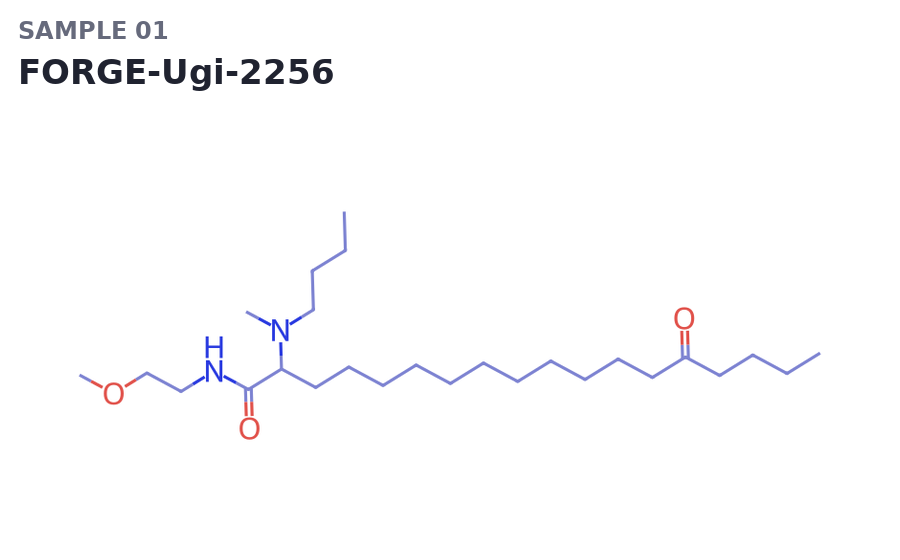
\includegraphics[width=\linewidth]{figures/forge_generated_samples_v2/forge_generated_sample_row_01_product.png}
\end{minipage}
&
\begin{minipage}[c][\samplerowheight][c]{\samplesemanticwidth}\centering
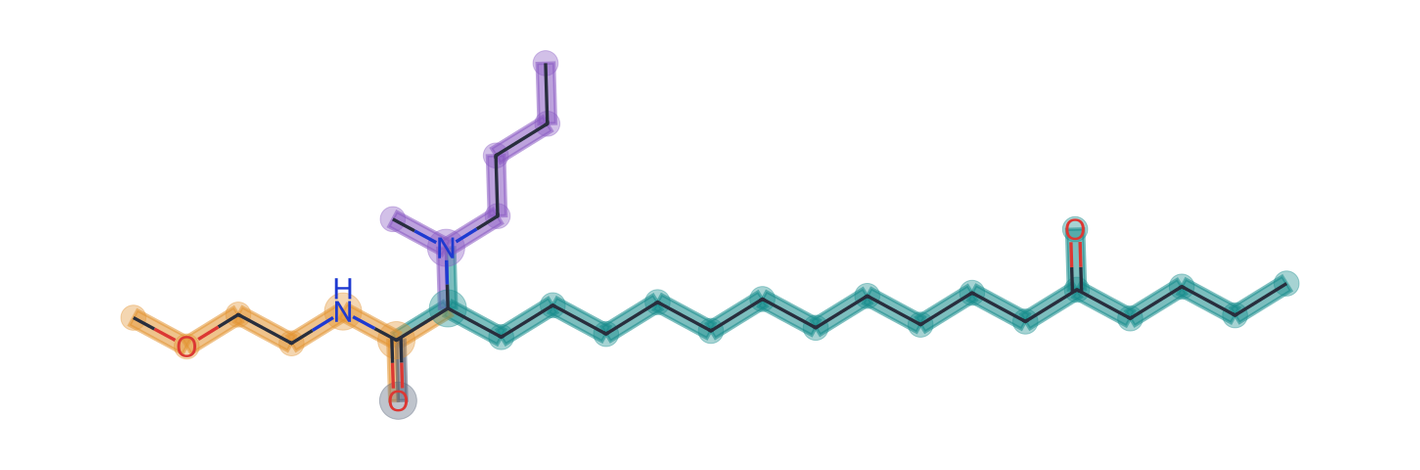
\includegraphics[width=\linewidth]{figures/forge_generated_samples_v2/forge_generated_sample_row_01_semantic.png}
\end{minipage}
&
\begin{minipage}[c][\samplerowheight][c]{\sampleprecursorwidth}\centering
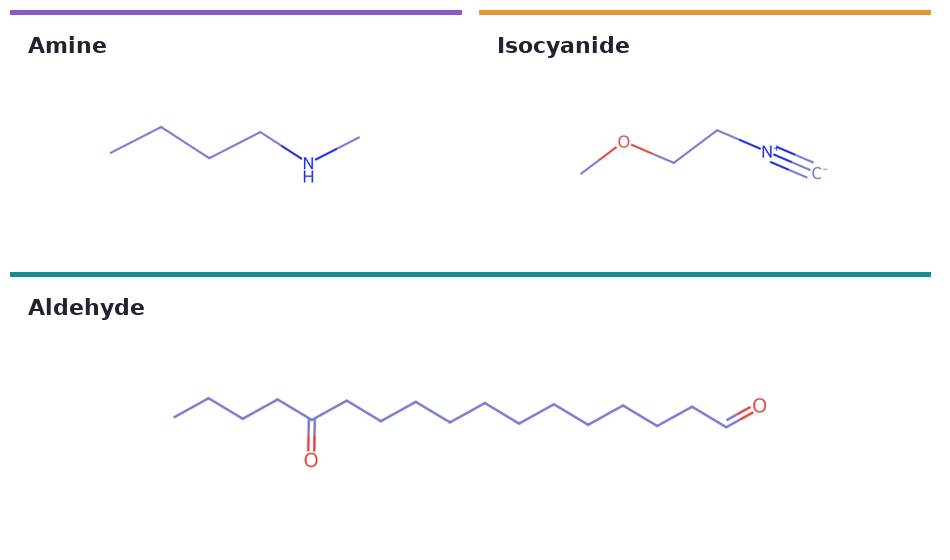
\includegraphics[width=\linewidth]{figures/forge_generated_samples_v2/forge_generated_sample_row_01_precursors.png}
\end{minipage}\\
\addlinespace[2.2mm]
\begin{minipage}[c][\samplerowheight][c]{\sampleproductwidth}\centering
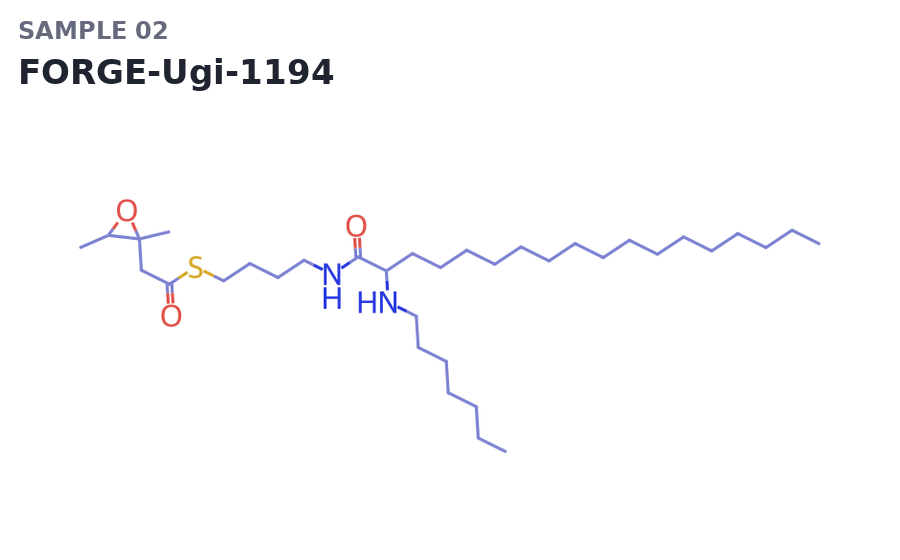
\includegraphics[width=\linewidth]{figures/forge_generated_samples_v2/forge_generated_sample_row_02_product.png}
\end{minipage}
&
\begin{minipage}[c][\samplerowheight][c]{\samplesemanticwidth}\centering
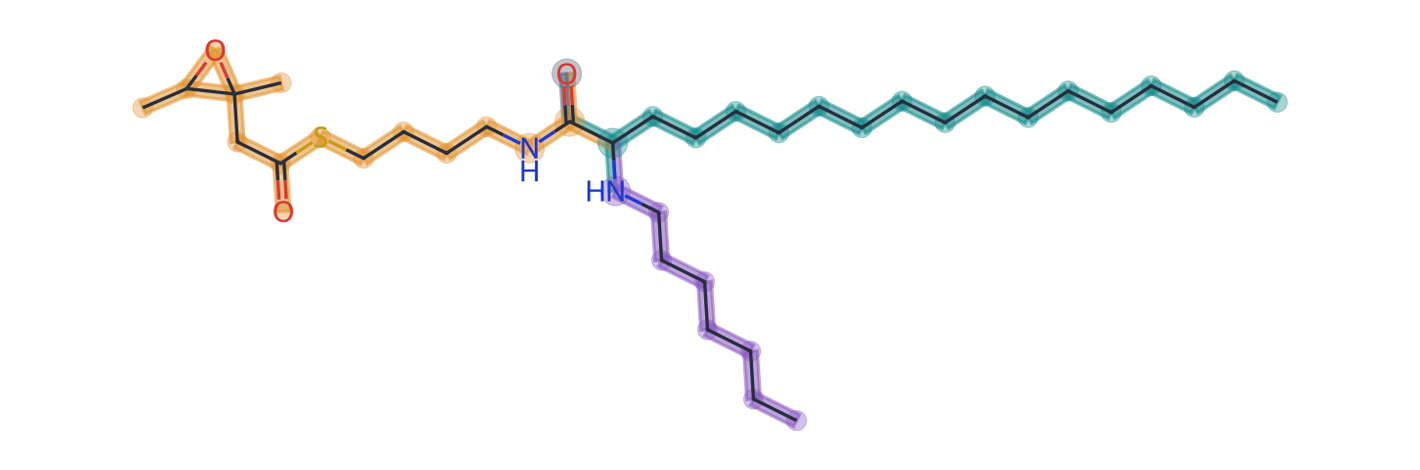
\includegraphics[width=\linewidth]{figures/forge_generated_samples_v2/forge_generated_sample_row_02_semantic.png}
\end{minipage}
&
\begin{minipage}[c][\samplerowheight][c]{\sampleprecursorwidth}\centering
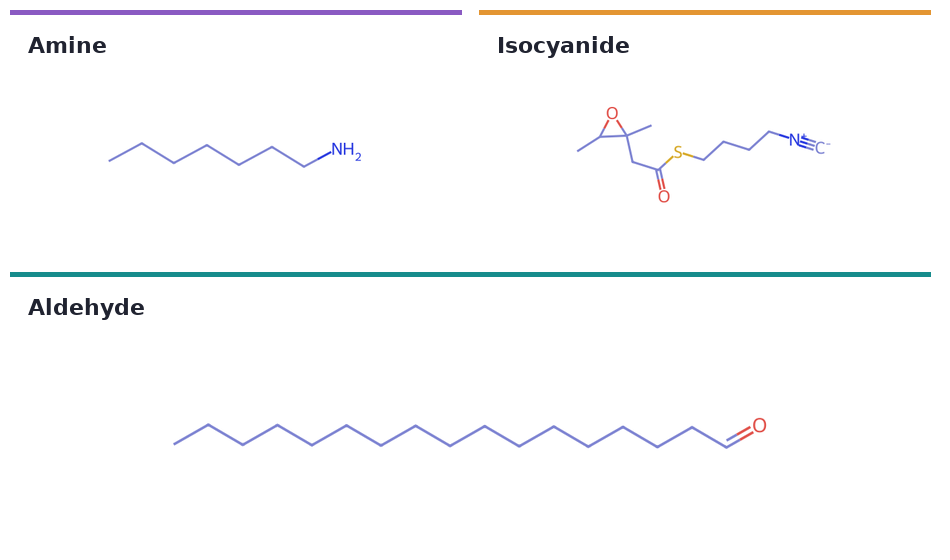
\includegraphics[width=\linewidth]{figures/forge_generated_samples_v2/forge_generated_sample_row_02_precursors.png}
\end{minipage}\\
\addlinespace[2.2mm]
\begin{minipage}[c][\samplerowheight][c]{\sampleproductwidth}\centering
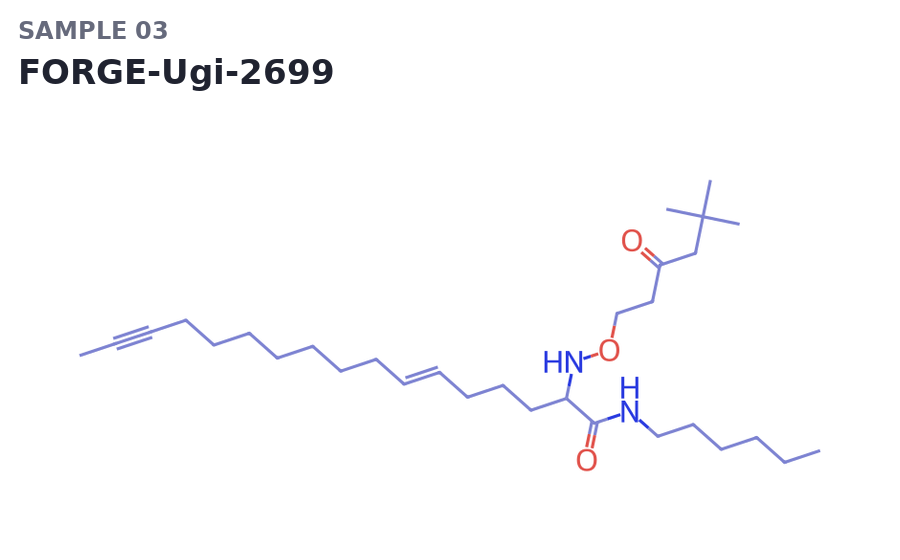
\includegraphics[width=\linewidth]{figures/forge_generated_samples_v2/forge_generated_sample_row_03_product.png}
\end{minipage}
&
\begin{minipage}[c][\samplerowheight][c]{\samplesemanticwidth}\centering
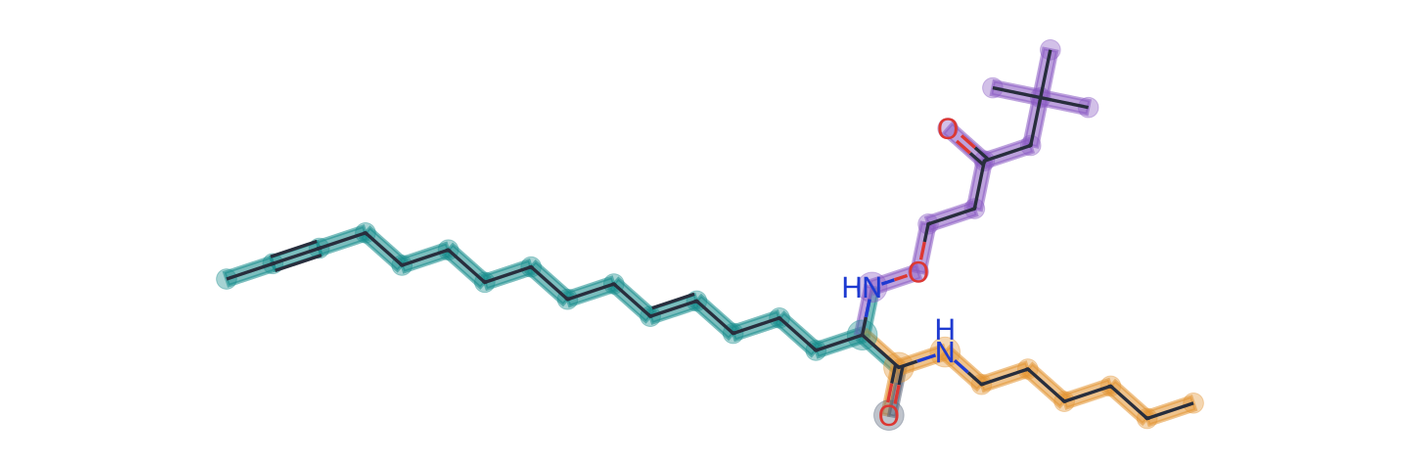
\includegraphics[width=\linewidth]{figures/forge_generated_samples_v2/forge_generated_sample_row_03_semantic.png}
\end{minipage}
&
\begin{minipage}[c][\samplerowheight][c]{\sampleprecursorwidth}\centering
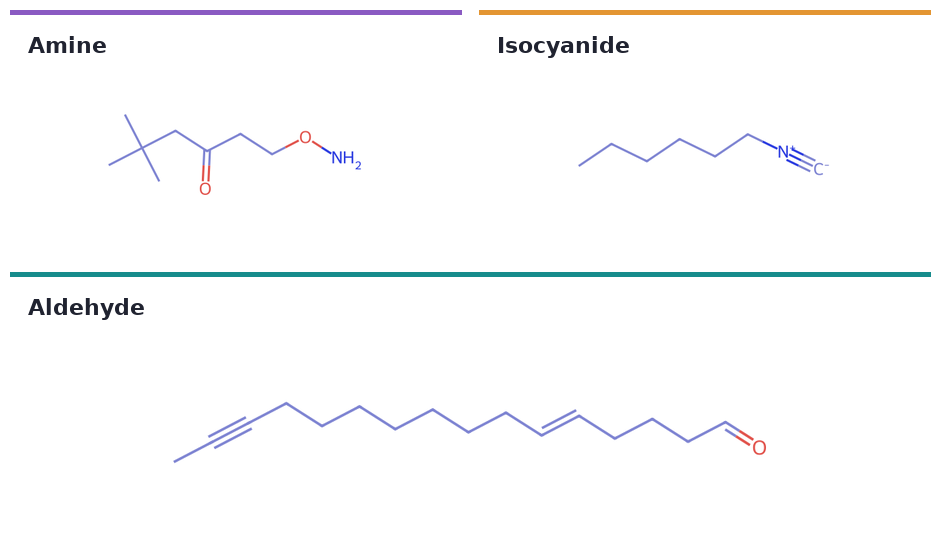
\includegraphics[width=\linewidth]{figures/forge_generated_samples_v2/forge_generated_sample_row_03_precursors.png}
\end{minipage}
\\
\addlinespace[0.6mm]
\bottomrule
\end{tabular}
}
\end{table}

\section{Discussion}

We present FORGE, a generative framework that uses known assembly chemistry during whole-molecule
generation while leaving precursor identities open. Across an AGILE-type Ugi three-component
reaction, repeated aza-Michael addition and repeated reductive amination, reaction-program
conditioning increased verified exact-L1 yield relative to matched whole-molecule generation followed by
post-hoc filtering, and FORGE generated exact assemblies whose verifier-returned traces contained
precursor identities absent from the corresponding training catalogues. Reaction information can
therefore guide molecular generation without making a finite component inventory part of the
generative state. Because direct catalogue-product reachability was not computed, this study does
not claim strong product-level catalogue escape.

The evidence is strongest for AGILE-type Ugi 3-CR; repeated aza-Michael addition is a second
computational family and repeated reductive amination a lighter stress test, showing lower exact-L1
yield, greater decomposition ambiguity and substantial between-seed variation. The study is
computational, supports only three qualified assembly programs and operates within a bounded
molecular graph space. Exact forward replay verifies structural consistency with the final assembly
reaction but does not establish precursor availability, experimental synthesis success, lipid
activity or RNA delivery, and the bounded HeLa diagnostic does not establish biological activity.
Several prespecified outcomes did not favor FORGE and are reported in full in
Appendix~\ref{app:results}: native recovery of specifically reserved held components remained weak at
\ForgeHeldComponentPerThousand{} products per 1,000 attempts, no evaluated method reproduced the
held-out observed-lipid distribution, joint denoising was not uniformly superior to role isolation
across programs, and neither synthesis tilting nor the nested potency proposal improved its matched
terminal endpoint. Prospective synthesis, formulation and biological validation are outside the
scope of this computational paper; none of the reported metrics should be interpreted as such
evidence. Within these limits, reaction programs provide a practical
coordinate system for expanding molecular identity without disconnecting generative design from
assembly chemistry.
\bibliography{../v0/forge,../v1/references}
\bibliographystyle{../v0/iclr2027_conference}

\clearpage
\appendix

\section{Preliminaries}
\label{app:preliminaries}

Appendices A through F are supplementary and are excluded from the five-page short-paper
limit, as are the references. They give the full formulation, the complete reporting contract, 
the theoretical results and a generated-structure atlas.

\subsection{Ionizable-lipid structure and modular assembly}

The structure of an ionizable lipid is typically organized into three functional regions: a
protonatable headgroup, a linker, and one or more hydrophobic domains
\citep{semple2010rational,jayaraman2012maximizing}.
Together, these regions determine the ionization, stability, lipid packing, and membrane
interactions of the molecule.
Ionizable-lipid libraries are often synthesized by applying a common reaction to different
combinations of precursor molecules
\citep{akinc2008combinatorial,love2010lipidlike,li2024accelerating,xu2024agile}.
Each precursor contributes a defined portion of the final lipid and contains the reactive group
required for the assembly.
The reaction forms the bonds that connect these precursor-derived regions.
As a result, the assembly reaction determines how the regions are connected, while the precursor
structures determine the molecular identity of the resulting lipid.

\subsection{Assembly chemistries studied}

We study three ionizable-lipid assembly chemistries: an AGILE-type
amine--aldehyde--isocyanide Ugi three-component reaction, repeated aza-Michael addition, and
repeated reductive amination.
In the AGILE-type Ugi reaction, an amine head reacts with an aldehyde component and an isocyanide
component to form an $\alpha$-amino amide that connects the headgroup to two hydrophobic regions
\citep{xu2024agile}.
A second assembly strategy uses repeated aza-Michael additions to attach acrylate-bearing
hydrophobic components sequentially to reactive amines in the headgroup
\citep{li2023combinatorial}.
Reductive amination sequentially couples aldehyde-bearing hydrophobic components to reactive amines
in the headgroup through new carbon--nitrogen bonds \citep{xue2024barcoding}.
Figure~\ref{fig:reaction-schemes} draws all three.

% [tbp] rather than [H]: the schemes are too tall to sit inline, and forcing them here broke the
% page early and left LaTeX stretching the section glue above to fill it.
\begin{figure}[tbp]
\centering
% The three assembly chemistries FORGE generates into, drawn natively so every glyph is the
% document's own font.  Colours follow the role palette of the algorithm schematic: the amine head
% is roleamine, aldehyde-derived atoms roleald, the isocyanide or acrylate tail roleiso, and an atom
% the template introduces with no precursor origin is grey, exactly as in the Figure 1 core inset.
% Skeletal notation throughout; hydrogens are drawn only on the atoms whose substitution decides
% whether the product can be decomposed back into its precursors.  Bonds carry the colour of the
% component that contributes them, so the reader can read the product back to its three sources.
\definecolor{roleamine}{HTML}{8A5AC2}
\definecolor{roleald}{HTML}{168C8C}
\definecolor{roleiso}{HTML}{E39532}
\definecolor{roletemplate}{HTML}{9A9A9A}
\setchemfig{atom sep=2.35em, bond style={line width=0.9pt}}
\newcommand{\amine}[1]{{\color{roleamine}#1}}
\newcommand{\ald}[1]{{\color{roleald}#1}}
\newcommand{\iso}[1]{{\color{roleiso}#1}}
\newcommand{\tmpl}[1]{{\color{roletemplate}#1}}
\newcommand{\rxnrow}[3]{%
  \makebox[\linewidth][l]{\begin{minipage}{\linewidth}%
  \textbf{\small #1}\\[-0.15em]{\scriptsize\itshape #2}\\[0.7em]#3\end{minipage}}}

\rxnrow{Ugi three-component reaction}
       {amine head, aldehyde and isocyanide combine in one step; no carboxylic-acid reactant component}{%
\schemestart
  \chemfig{R^1-[:30]\amine{N}(-[:90]R^2)-[:-30]\amine{H}}
  \+
  \chemfig{R^3-[:30,,,,roleald]\ald{CH}=[:-30,,,,roleald]\ald{O}}
  \+
  \chemfig{R^4-[:30,,,,roleiso]\iso{N}~[:-30,,,,roleiso]\iso{C}}
  \arrow{->}
  \chemfig{R^1-[:30,,,,roleamine]\amine{N}(-[:90,,,,roleamine]R^2)-[:-30,,,,roleald]\ald{CH}(-[:-90,,,,roleald]R^3)-[:30,,,,roleiso]\iso{C}(=[:90,,,,roletemplate]\tmpl{O})-[:-30,,,,roleiso]\iso{NH}-[:30,,,,roleiso]R^4}
\schemestop}\par

\par\vspace{1.9em}\par
\rxnrow{Repeated aza-Michael addition}
       {the head N--H adds across the acrylate double bond; the ester is untouched}{%
\schemestart
  \chemfig{R^1-[:30]\amine{N}(-[:90]R^2)-[:-30]\amine{H}}
  \+
  \chemfig{-[:30,,,,roleiso]=[:-30,,,,roleiso]-[:30](=[:90]O)-[:-30]O-[:30]R^3}
  \arrow{->}
  \chemfig{R^1-[:30,,,,roleamine]\amine{N}(-[:90,,,,roleamine]R^2)-[:-30,,,,roleiso]-[:30,,,,roleiso]-[:-30](=[:90]O)-[:30]O-[:-30]R^3}
\schemestop}\par

\par\vspace{1.9em}\par
\rxnrow{Repeated reductive amination}
       {one new carbon--nitrogen bond; the carbonyl oxygen leaves as water}{%
\schemestart
  \chemfig{R^1-[:30]\amine{N}(-[:90]R^2)-[:-30]\amine{H}}
  \+
  \chemfig{R^3-[:30,,,,roleald]\ald{CH}=[:-30,,,,roleald]\ald{O}}
  \arrow{->[\scriptsize$-\,$H$_2$O]}
  \chemfig{R^1-[:30,,,,roleamine]\amine{N}(-[:90,,,,roleamine]R^2)-[:-30,,,,roleald]-[:30,,,,roleald]R^3}
\schemestop}

\caption{\textbf{The three assembly chemistries.} Skeletal notation, with each bond carrying the
colour of the component that contributes it: amine head in purple, aldehyde-derived atoms in teal,
the isocyanide or acrylate tail in orange. Grey marks an atom the assembly template introduces and
no precursor supplies, following the same convention as the core inset of
Figure~\ref{fig:forge-overview}. Hydrogens are drawn only on the atoms whose substitution decides
whether a product can be decomposed back into precursors: the head N--H, and the
$\alpha$-carbon C--H that the Ugi reaction takes from the aldehyde. $R^i$ stand for the
source-linked components of the frozen library, which are larger than the fragments drawn here.
The Ugi variant has no carboxylic-acid reactant component.}
\label{fig:reaction-schemes}
\end{figure}

\subsection{Reaction transforms and exact assembly}

Each assembly chemistry defines a forward transformation that maps role-assigned precursor
molecules to the product graphs permitted by that reaction.
The corresponding reverse transformation decomposes a complete lipid into the precursor
assignments that could have produced it.
To verify a decomposition, we computationally replay the reaction on the recovered precursors.
The product passes the level-one (L1) assembly check only if the reconstruction matches the original
lipid exactly.

\subsection{Discrete molecular graph spaces}

Let $\Sigma_{\rm atom}$ and $\Sigma_{\rm bond}$ be finite atom-state and bond-state vocabularies.
A molecular graph is $G=(V,E,\ell_V,\ell_E)$, where the underlying graph is finite, connected,
undirected and simple, $\ell_V:V\to\Sigma_{\rm atom}$, and
$\ell_E:E\to\Sigma_{\rm bond}$. Bond order is part of $\ell_E$ rather than a parallel edge.
Graphs are identified up to label-preserving isomorphism. The declared model support additionally
bounds the heavy-atom count and cycle rank.

\subsection{Discrete flow matching}

For one coordinate with alphabet $\mathcal X_i$, full-support source marginal $q_{0,i}$ and clean
endpoint $a\in\mathcal X_i$, the linear conditional path is
\begin{equation}
    q_{t\mid1,i}(u\mid a)
    = (1-t)q_{0,i}(u) + t\,\mathbf 1\{u=a\},
    \qquad t\in[0,1],
\end{equation}
with a univariate conditional rate $R^*_{t,i}(u,v\mid a)$ that realizes this path
\citep{qin2025defog}. FORGE applies this construction independently to the variable coordinates
conditional on the shared clean endpoint. Consequently the joint conditional path is a product of
coordinate paths, not the mixture $(1-t)q_0+tq_1$. Its continuous-time generator permits one
coordinate jump at an infinitesimal time. The denoiser predicts the clean posterior marginal of each
coordinate, which is exactly the quantity needed to marginalize the corresponding local rate.
Appendix~\ref{app:forge} defines the full path, learned generator and the capped
independent-coordinate Euler approximation used in code.

\clearpage

\section{FORGE in full}
\label{app:forge}

This appendix gives the complete formulation summarized in Section~2 of the body.

\subsection{Overview}

We formulate ionizable-lipid design as conditional generation under a specified reaction program,
while leaving precursor identities unspecified.
Let $G\in\mathcal{G}$ denote a complete ionizable-lipid graph and $P\in\mathcal{P}$ a reaction
program specifying the assembly chemistry, precursor roles, reaction-core positions, and
transformation order.
FORGE models the conditional distribution $p_\theta(G\mid P)$ without access to precursor
identifiers, stored component graphs, or fragment tokens.
FORGE is organized into four stages:
\begin{enumerate}
    \item \textbf{Reaction-program specification.}
    $P$ defines the assembly chemistry, precursor roles, reaction-core positions, transformation
    order, and coarse per-role morphology, but not precursor identities.

    \item \textbf{Whole-graph generation.}
    A conditional discrete flow generates every atom, bond, and topology state of $G$ under $P$.

    \item \textbf{Exact assembly verification.}
    A reverse transform decomposes $G$ into role-assigned precursors, and the corresponding forward
    transform must reconstruct $G$ exactly.

    \item \textbf{Recursive synthesis-program construction.}
    FORGE searches for preparation routes to generated precursors that are not already supported as
    available starting materials and abstains when a route cannot be completed.
\end{enumerate}




\subsection{Synthesis-grounded design task}

Given a reaction program $P$, FORGE must generate a complete molecular graph $G$ and either
construct a complete synthesis program for $G$ or abstain.
Let $\mathfrak D$ denote the dossier space and let $\mathfrak F_{\mathfrak B}$ be the finite set of
typed failure outcomes under a frozen route contract $\mathfrak B_{\rm route}$.
We write the design process as
\begin{equation}
    G\sim p_\theta(\cdot\mid P),
    \qquad
    Y=\mathsf{Assess}_{\mathfrak B}(G,P,\mathbf C_T,\tau_T)
    \in\mathfrak D\cup\mathfrak F_{\mathfrak B}.
\end{equation}
$\mathsf{Assess}_{\mathfrak B}$ denotes the bounded program constructor, invoked after the verifier
selects the sole admitted root trace $(\mathbf C_T,\tau_T)\in\widehat{\mathcal E}_P(G)$, that verifies the final
assembly, searches for preparation routes to unavailable precursors, and checks terminal supplier
evidence. $P$ and the assessor act at different stages: $P$ guides generation, whereas the assessor
constructs a dossier from the completed graph without modifying it.
FORGE accepts $(G,T)$ only when $G$ passes molecular and exact-assembly verification and $T$ traces
every required precursor to an available starting material; otherwise, it abstains.

\subsection{Reaction-program specification}

\begin{definition}[Reaction program]
A reaction program is a tuple
\begin{equation}
    P=(c,d,\mathbf{r},\mathbf{k},M),
\end{equation}
with an ordered layout index set $\mathcal I(P)=\{1,\ldots,n(P)\}$. Here $c$ identifies the
ordered assembly chemistry, $d$ is the program depth,
$\mathbf r=(r_i)_{i\in\mathcal I(P)}$ assigns precursor roles,
$\mathbf k=(k_i)_{i\in\mathcal I(P)}$ marks reaction-core positions, and $M$ specifies coarse
per-role morphology.
For each precursor role $r$, $M$ records four integers: the number of exterior atoms $n_r$,
junction budget $j_r$, cycle rank $\gamma_r$, and attachment count $a_r$.
\end{definition}
$M$ is defined relative to an exact atom-mapped trace $\tau$ and precursor tuple $\mathbf C$.
An atom is exterior for role $r$ when $\tau$ assigns it to the corresponding precursor and does not
mark it as reaction core. Template-introduced atoms belong to the core and to no precursor role.
The role-induced subgraph contains the atoms assigned to $r$ and all product bonds with both
endpoints in that set. Its junction count is
$\sum_v\max\{\deg_r(v)-2,0\}$, its cycle rank is
$|E_r|-|V_r|+\kappa_r$ for $\kappa_r$ connected components, and its core-attachment count is the
number of product bonds between an exterior atom of $r$ and a core atom. We write
$(G,\mathbf C,\tau)\models M(P)$ when these values match the sampled counts, with junction count at
most its budget. Thus morphology is decomposition-relative rather than an unlabeled property of
$G$.

FORGE first samples an admissible complete program $P$ from the training-fold program prior and then
generates $G$ conditioned on it:
\begin{equation}
    p_\theta(G,P\mid c)
    = p_{\mathrm{prog}}(P\mid c)\,p_\theta(G\mid P).
\end{equation}
The prior sets each region's atom count, branching budget, cycle rank, and number of core
attachments, but not its molecular structure.
A chemistry-specific adapter defines the precursor roles, reaction core, reverse decomposition, and
forward transform associated with $c$.
For each graph position $i$, FORGE combines learned embeddings of the program identity, program
depth, precursor role, and reaction-core position:
\begin{equation}
    h_i^P
    = \operatorname{LN}\!\left(
        e_c(c) + e_d(d) + e_r(r_i) + e_k(k_i)
        + \sum_{u=1}^{4}e_{M,u}(M_{r_i,u})
    \right).
\end{equation}
The morphology fields also determine active positions and fixed/variable masks in the sampling
layout. These coordinates tell the generator which precursor role each position plays, whether it
lies in the reaction core, and the role-local count constraints, but not which molecular structure
should occupy that role.

\subsection{Program-defined molecular space}

Reaction programs constrain how a lipid is assembled without specifying the molecular structures
that occupy its precursor roles.
Let $\mathcal{G}_{\mathrm{bounded}}\subseteq\mathcal{G}$ denote the molecular graphs within the
declared atom and bond vocabularies, the 194-heavy-atom limit, and the three-closure limit.
For chemistry $c$, let $\mathcal D_c(G)$ be the candidate exact-decomposition search space and define
\begin{equation}
    \mathcal D_P(G)
    =\left\{(\mathbf C,\tau)\in\mathcal D_c(G):
    (G,\mathbf C,\tau)\models P\right\}.
\end{equation}
The valid, exact-L1 molecular space associated with $P$ is
\begin{equation}
    \mathcal{G}_{\mathrm{L1}}(P)
    =
    \left\{
        G\in\mathcal{G}_{\mathrm{bounded}}:
        \mathrm{Valid}(G)=1,\;
        \widehat{\mathrm{L1}}(G,P)=1
    \right\}.
\end{equation}
A generated lipid can pass the exact L1 check even when one or more recovered precursors never
appeared in the training component set, provided the specified reaction reconstructs the lipid from
them.
For a reaction program $P$, let $\mathfrak C_P$ denote its admissible precursor-program inputs, including
precursor identities, role assignments, and program depth.
The registered forward operator maps each input to a finite set of canonical products:
\begin{equation}
    \mathcal{F}_P:
    \mathfrak C_P
    \longrightarrow
    2^{\mathfrak{G}_{N,K_{\rm cl}}}.
\end{equation}
Given role-specific catalogues $\mathcal C$, let
$\mathfrak C_P(\mathcal C)\subseteq\mathfrak C_P$ contain the admissible program inputs whose
components all belong to their corresponding catalogues.
The catalogue-reachable product set is
\begin{equation}
    \mathcal{G}_{\mathrm{cat}}(P,\mathcal C)
    =
    \bigcup_{\mathbf C\in\mathfrak C_P(\mathcal C)}
    \mathcal{F}_P(\mathbf C).
\end{equation}
For any graph $G$, define its complete program-relative preimage as
\begin{equation}
    \mathcal{E}^{\star}_P(G)
    =
    \left\{
        \mathbf C\in\mathfrak C_P:
        G\in\mathcal{F}_P(\mathbf C)
    \right\}.
\end{equation}

\begin{definition}[Strong catalogue escape]
\label{def:catalogue-escape}
\begin{equation}
    \operatorname{Escape}^{\star}(G;P,\mathcal C)
    =
    \mathbf{1}\!\left[
        \mathcal E_P^\star(G)\neq\varnothing
        \;\land\;
        \mathcal E_P^\star(G)\cap\mathfrak C_P(\mathcal C)=\varnothing
    \right].
\end{equation}
\end{definition}
Proposition~\ref{prop:catalogue-bound} bounds the catalogue-reachable product set.
For a verified exact-L1 graph, direct membership in the canonical product-hash set gives the
operational strong-escape test
\begin{equation}
    \mathrm{StrongEscape}(G;P,\mathcal C)
    =\mathbf 1\!\left[
       \widehat{\mathrm{L1}}(G,P)=1\ \land\
       G\notin\mathcal G_{\rm cat}(P,\mathcal C)
    \right].
\end{equation}
The verifier-returned set $\widehat{\mathcal E}_P(G)$ defined below is a subset of
$\mathcal E_P^\star(G)$ when every returned trace passes exact forward replay.
A novel component in a returned trace establishes strong catalogue escape only when reverse
enumeration is exhaustive or direct catalogue reachability is checked independently.
The present experiments did not precompute a complete common-reference product-hash set, so they
report verifier-recovered component novelty as a secondary diagnostic and do not report
$\mathrm{StrongEscape}$ for FORGE.
FORGE instead parameterizes $p_\theta(G\mid P)$ over whole graphs in
$\mathcal{G}_{\mathrm{bounded}}$, without including any component catalogue $\mathcal{C}_r$ in the
generative state.
Reaction programs constrain assembly semantics, while the flow determines precursor identity at atom
and bond resolution.

\subsection{Whole-graph generation}

FORGE realizes this whole-graph distribution with a discrete flow over atom, bond, and topology
states.
To preserve the full 194-atom support without an $O(N_{\max}^2)$ edge state, FORGE encodes each
graph as a spanning tree plus at most three residual closure edges.
Let $\alpha=(\mathbf C,\tau,\mathbf r,\mathbf k)$ contain the selected exact precursor tuple,
atom-mapped reaction trace, precursor-role assignment and reaction-core annotation. The deterministic
program-aware encoder
\begin{equation}
    \operatorname{Enc}_P:
    \{(G,\alpha):G\in\mathfrak G_{N_{\max},K_{\rm cl}}
      \text{ and }\alpha\text{ is admitted for }P\}
    \longrightarrow \mathfrak X_{N_{\max},K_{\rm cl}}
\end{equation}
constructs the categorical graph state
\begin{equation}
    X_G:=\operatorname{Enc}_P(G,\alpha)=
    \left(
        \mathbf{a},
        \boldsymbol{\pi},
        \mathbf{b},
        \mathbf{e}^{L},
        \mathbf{e}^{R},
        \mathbf{z}
    \right)
\end{equation}
where $\mathbf{a}$ contains atom states, $\boldsymbol{\pi}$
parent pointers, $\mathbf{b}$ spanning-tree bond states, $\mathbf{e}^{L}$ and $\mathbf{e}^{R}$
closure-endpoint pointers, and $\mathbf{z}$ closure-bond states.

The encoder first partitions the atoms into connected precursor-origin components under $\alpha$.
It chooses as root the reaction-core atom with the smallest tied-broken canonical RDKit rank, and
orders the origin-component graph by breadth-first traversal from that root component, breaking
ties by role index, component canonical ranks and original atom index. Within each component it uses
a deterministic depth-first preorder from the selected attachment atom, with neighbors ordered by
the same canonical ranks. The traversed bonds define the spanning tree. Every residual bond is
represented once as an ordered endpoint pair with its bond label, and residual triples are sorted
lexicographically. Role, core, fixed-coordinate and morphology arrays are permuted by precisely the
same atom order. Training records with more than one qualified exact source trace are not resolved
arbitrarily: they abstain from semantic training; duplicate descriptions of the same admitted trace
collapse to its canonical record. Thus
$\operatorname{Dec}(\operatorname{Enc}_P(G,\alpha))\cong G$ for every admitted record.

The raw padded categorical product space $\overline{\mathfrak X}_{N_{\max},K_{\rm cl}}$ also
contains malformed states. Its well-formed subset $\mathfrak X_{N_{\max},K_{\rm cl}}$ enforces an
active node prefix, earlier-parent pointers, distinct valid closure endpoints, no duplicate edges,
and null values in unused closure slots. The partial decoder is therefore typed as
\begin{equation}
    \operatorname{Dec}:\overline{\mathfrak X}_{N_{\max},K_{\rm cl}}
    \longrightarrow
    \mathfrak G_{N_{\max},K_{\rm cl}}\cup\{\bot_{\rm dec}\}.
\end{equation}
For this study, $N_{\max}=194$ and $K_{\rm cl}=3$.
This is a statement about architectural support.
It does not imply reaction consistency, nonzero probability under a trained model, or
synthesis-program completeness.

If $q_\theta(x\mid P)$ is the terminal raw-state law, the generated graph distribution is its
decoder pushforward,
\begin{equation}
    p_\theta([G]_{\cong}\mid P)
    =\sum_{x:\operatorname{Dec}(x)\cong G}q_\theta(x\mid P),
    \qquad
    p_\theta(\bot_{\rm dec}\mid P)
    =\sum_{x:\operatorname{Dec}(x)=\bot_{\rm dec}}q_\theta(x\mid P).
\end{equation}

The chemistry adapter marks any atom, pointer, or bond states fixed by $P$.
FORGE holds these states constant while corrupting the remaining states along the linear probability
path and predicting their clean values from $(X_t,t,P)$. Let $\Omega_P$ be the face of the raw state
space satisfying those fixed coordinates, and define the admissible program set
\begin{equation}
    \mathcal P_{\rm adm}
    =\left\{P:\mathfrak X_{N_{\max},K_{\rm cl}}\cap\Omega_P\neq\varnothing\right\}.
\end{equation}
The morphology prior is normalized only on $\mathcal P_{\rm adm}$. Each chemistry adapter is required
to satisfy the program-compatible encoding property: every admitted annotated record obeys
$\operatorname{Enc}_P(G,\alpha)\in\Omega_P$. Corpus construction checks this invariant together
with exact constitutional decode round trip and fails closed before a record enters any split. This
is an exhaustive implementation invariant over the cached training, calibration and held-out
records, not a theorem for unregistered chemistries.

Let $\mathscr J=\{\mathbf{a},\boldsymbol{\pi},\mathbf{b},\mathbf{e}^{L},\mathbf{e}^{R},\mathbf{z}\}$
denote the six state families optimized during training.
Let $\mu_{\mathrm{bal}}$ denote the frozen training distribution over graph-program pairs, which
assigns equal total mass to each reaction program and preserves the source-balanced weights within
each program.
For each $q\in\mathscr J$, let $m_j^{(q)}(P)\in\{0,1\}$ indicate whether coordinate $j$ remains
variable under $P$.
FORGE minimizes a program-balanced denoising objective over the variable coordinates:
\begin{equation}
\begin{aligned}
    \mathcal{L}_{\mathrm{FORGE}}(\theta)
    & = \mathbb{E}_{\substack{
        (G,P)\sim\mu_{\mathrm{bal}},\;
        t\sim\mathcal{U}(0,1),\;
        X_t\sim p_t(\cdot\mid X_G,P)
    }}
    \Bigg[
    \\
    & \quad
        \sum_{q\in\mathscr J}
        \lambda_q
        \frac{
            \sum_j m_j^{(q)}(P)
            \left[-\log p_\theta\!\left(X_{G,j}^{(q)}\mid X_t,t,P\right)\right]
        }{
            \max\!\left\{1,\sum_j m_j^{(q)}(P)\right\}
        }
    \Bigg].
\end{aligned}
\end{equation}
Here, $\lambda_q$ weights state family $q$, and a family with no variable coordinates contributes
zero loss.
The corruption and sampling operators assign zero rates to program-fixed coordinates and project
each finite-step state back onto them as an implementation safeguard. This is the precise syntactic
sense in which the program constrains a state trajectory: fixed coordinates cannot be resampled.
Chemical consistency with the requested assembly is established separately by exact forward replay.
Under an unrestricted coordinatewise model class, every population minimizer of the primary masked
denoising term recovers the corresponding clean-coordinate posterior marginals. This result does
not characterize the optimizer of the auxiliary-loss or PCGrad procedure
(Propositions~\ref{prop:fixed-invariance} and~\ref{prop:masked-bayes}).

The denoiser is a graph Transformer over the complete sparse state. Each layer applies graph
self-attention with relation biases for parent, child and closure edges, then cross-attends to memory
tokens representing program identity, program depth, precursor role and reaction-core position.
Cross-attention is repeated in every layer so that reaction semantics can influence both local state
updates and long-range coordination among precursor-derived regions. Three softly program-routed
residual adapters provide family-specific capacity while retaining a shared whole-graph backbone.

For each reaction family $f$, we compute a task loss
\begin{equation}
    \mathcal L_f
    = \mathcal L_{\mathrm{FORGE},f}
    + \lambda_{\mathrm{role}}\mathcal L_{\mathrm{role}}
    + \lambda_{\mathrm{core}}\mathcal L_{\mathrm{core}}.
\end{equation}
Present semantic states receive equal mass within each auxiliary term. Training gives every reaction
family equal total loss mass. The gradients of the family task losses, not the individual loss
heads, are combined by deterministic PCGrad. Families are ordered by their integer program state.
Writing $g_f=\nabla_\theta\mathcal L_f$, the algorithm initializes
$\widetilde g_f\leftarrow g_f$ and, for every other family $h$ in that fixed order, applies
\begin{equation}
    \widetilde g_f\leftarrow
    \widetilde g_f-
    \mathbf 1\{\langle\widetilde g_f,g_h\rangle<0\}
    \frac{\langle\widetilde g_f,g_h\rangle}{\max(\lVert g_h\rVert_2^2,10^{-12})}
    g_h
\end{equation}
on parameter coordinates available to both tasks. Zero gradients remain zero; gradients are not
norm-normalized; and the optimizer receives the arithmetic mean of the projected family gradients.
This is an algorithmic definition of the update and is not the gradient of the displayed scalar
sum in general.
Table~\ref{tab:architecture-ablations} prespecifies separate interventions for layerwise
cross-attention, each auxiliary loss, routed adapters and gradient conflict control.

At inference, FORGE samples $X_0$ from the factorized program-compatible source, assigns zero update
rates to fixed coordinates, and applies $L_{\rm samp}$ capped independent-coordinate Euler steps.
At each step the implementation samples one clean category per coordinate from the denoiser, forms
the minimum $R^*$ rate for that sampled endpoint, multiplies it by
$\Delta t=1/L_{\rm samp}$, and rescales the total off-diagonal mass to at most $0.999$ before drawing
the next coordinate value. This is a finite-step Monte Carlo approximation to the local CTMC, not
exact CTMC simulation. Appendix~\ref{app:theory} states the ideal marginalized rate and the numerical
kernel.
FORGE decodes the terminal state $X_1$ into a molecular graph $G$ and retains it only if it is
connected, valence-valid, and passes molecular sanitization.

\subsection{Exact assembly verification}

To ensure that each retained graph satisfies the specified reaction program, FORGE decomposes it
into role-assigned precursors and applies the corresponding forward transform.

\begin{definition}[Mathematical and verifier-relative L1]
For chemistry $c$, the reverse search $\mathcal D_c$ maps $G$ to candidate role-assigned precursor
tuples and atom-mapped traces. The complete mathematical preimage $\mathcal E_P^\star(G)$ contains
every admissible input whose registered forward operator can produce $G$. Define
\begin{equation}
    \mathrm{L1}^\star(G,P)
    =\mathbf 1\!\left[\mathcal E_P^\star(G)\neq\varnothing\right].
\end{equation}
The bounded implementation searches $\mathcal D_P(G)\subseteq\mathcal D_c(G)$ and returns
\begin{equation}
    \widehat{\mathcal E}_P(G)
    =
    \left\{
        (\mathbf C,\tau)\in\mathcal D_P(G):
        \exists H\in\mathcal F_P(\mathbf C)\text{ such that }H\cong G
    \right\}.
\end{equation}
Its verified predicate is
\begin{equation}
    \widehat{\mathrm{L1}}(G,P)
    = \mathbf{1}\!\left[
        \widehat{\mathcal E}_P(G)\neq\varnothing
    \right].
\end{equation}
\end{definition}
Every returned trace passes exact replay, hence
$\widehat{\mathrm{L1}}(G,P)\leq\mathrm{L1}^\star(G,P)$. Reverse-search completeness has not been
proved, so the reported metric is called \emph{verified exact-L1 yield}.
Post-hoc filtering changes which completed samples are retained but cannot change the proposal
distribution's exact-L1 acceptance probability.
Under independent sampling, this probability determines the complete distribution of accepted
counts under a fixed attempt budget and the expected cost of obtaining a fixed number of accepted
products (Proposition~\ref{prop:posthoc-budget}).
FORGE reports decomposition coverage separately from forward-replay precision because identifying a
candidate disconnection does not guarantee exact reconstruction of $G$.
Candidate decomposition coverage is the fraction of valid graphs for which
$\mathcal D_c(G)\neq\varnothing$. Candidate replay precision is
\begin{equation}
 \mathrm{ReplayPrecision}
 =\frac{\sum_G\sum_{(\mathbf C,\tau)\in\mathcal D_P(G)}
 \mathbf 1\{\exists H\in\mathcal F_P(\mathbf C):H\cong G\}}
 {\sum_G|\mathcal D_P(G)|},
\end{equation}
with N/E when the denominator is zero. Replay of tuples already in
$\widehat{\mathcal E}_P(G)$ is a $100\%$ verifier invariant rather than an empirical precision
result. We separately define
\begin{equation}
 \mathrm{CandidateAmbig}(G,c)=\mathbf 1\{|\mathcal D_c(G)|>1\},\qquad
 \mathrm{ExactAmbig}(G,P)=\mathbf 1\{|\widehat{\mathcal E}_P(G)|>1\}.
\end{equation}
A distinct exact-L1 product is a deduplicated generated constitution; an unambiguous exact
decomposition instead has $|\widehat{\mathcal E}_P(G)|=1$. We do not use ``unique L1'' for both.

\subsection{Recursive synthesis-program construction}

The final assembly requires access to every recovered precursor.
Exact L1 verification identifies these precursors, but it does not establish whether they are
available or how to prepare them.
For laboratory planning, an exact final assembly is useful only when every required precursor is
either available or connected to available starting materials through a supported preparation
route.
Let $T=(V_M,V_R,E)$ denote a bipartite synthesis tree rooted at $G$, where each product molecule
points to its preparation reaction and each reaction points to its required reactants.
FORGE constructs these routes recursively and rejects the lipid when any branch remains unresolved.
A molecule node terminates when a current, dated supplier record lists an exact constitutional match
as available; otherwise, FORGE must expand that node through a supported, forward-verified reaction.
FORGE uses a bounded level-two (L2) planner to propose each expansion.
For each proposal, FORGE records the reaction, reactants, product, and supporting evidence, and
accepts the step only when the forward transform reconstructs the target precursor exactly.
Each accepted reaction adds its reactants as new molecule nodes, and FORGE applies the same
termination-or-expansion rule recursively.
The current assessor admits only an unambiguous verified exact-L1 root. Every dossier therefore
records the sole selected root trace
$(\mathbf C_T,\tau_T)\in\widehat{\mathcal E}_P(G)$; an ambiguous exact set produces a typed
abstention. For each upstream reaction node $r$, let
$\mathrm{Admitted}_{\mathfrak B}(r)=1$ when its reaction and substrate scope satisfy the frozen
evidence policy, and let $\mathrm{Verify}_{\mathfrak B}(r)=1$ when
$\operatorname{target}(r)\in\mathcal F_r(\operatorname{reactants}(r))$.
For each leaf molecule $\ell$, let $\mathrm{Available}_{\mathfrak B}(\ell)=1$ when it satisfies the terminal
supplier-evidence rule.
Let $V_R^{\mathrm{up}}(T)$ denote the upstream preparation-reaction nodes and $L(T)$ the leaf
molecules. $\mathrm{WellFormed}(G,T,P)$ requires that $T$ is a connected, acyclic bipartite tree
rooted at $G$; each internal molecule has exactly one recorded producing reaction; each reaction's
incoming molecule children equal its recorded reactants; and $T$ has no disconnected, cyclic or
extraneous node. Its distinguished final-assembly record must have product $G$ and precursor
children exactly $\mathbf C_T$ under trace $\tau_T$.
\begin{equation}
\begin{aligned}
    \mathrm{Complete}_{\mathfrak B}(G,T,P)
    ={}&\mathrm{WellFormed}(G,T,P)
    \mathbf 1\!\left[(\mathbf C_T,\tau_T)\in\widehat{\mathcal E}_P(G)\right]\\
    &\times\prod_{r\in V_R^{\mathrm{up}}(T)}
    \mathrm{Admitted}_{\mathfrak B}(r)\mathrm{Verify}_{\mathfrak B}(r)
    \prod_{\ell\in L(T)}\mathrm{Available}_{\mathfrak B}(\ell).
\end{aligned}
\end{equation}
Empty products equal one. Let $\mathfrak B_{\rm route}$ fix the route-depth and query budgets,
registered transforms, evidence-admission policy, and dated supplier snapshot used by
$\mathsf{Assess}_{\mathfrak B}$.
Under finite search bounds and terminating evidence queries, the assessor terminates and returns a
dossier only when $\mathrm{Complete}_{\mathfrak B}(G,T,P)=1$
(Lemma~\ref{lem:planner-termination} and Invariant~\ref{inv:dossier-soundness}).
An abstention means that FORGE did not complete a dossier under $\mathfrak B_{\rm route}$; it does not imply that
no synthesis route exists outside the frozen search space or evidence snapshot.
The guarantee is computational and does not establish experimental synthesis success.

Algorithm~\ref{alg:forge-inference} summarizes the complete inference procedure.
Every iteration consumes one generation attempt, and FORGE retains the outcome of every failed
attempt in a typed ledger.
\begin{algorithm}[t]
\caption{FORGE generation and fail-closed synthesis-program construction.}
\label{alg:forge-inference}
\begin{algorithmic}[1]
\Require trained coordinate predictors, reaction program $P$, Euler-step count $L_{\rm samp}$,
attempt budget $B$, recorded seed $s$, and frozen route contract $\mathfrak B_{\rm route}$
\Ensure attempt-indexed dossier sequence $\mathcal D_{\rm out}$, exact-L1 ledger $\mathcal L_{\rm out}$,
and typed failure ledger $\mathcal H$
\State initialize the random-number streams from $s$;
$\mathcal D_{\rm out}\gets[\,]$; $\mathcal L_{\rm out}\gets[\,]$; $\mathcal H\gets[\,]$
\For{$b=1,\ldots,B$}
    \State sample $X_0\sim q_0^P$ and set $X\gets\Pi_P(X_0)$
    \For{$k=0,\ldots,L_{\rm samp}-1$}
        \State $t_k\gets k/L_{\rm samp}$; $\Delta t_k\gets1/L_{\rm samp}$
        \State $X\gets\Pi_P\!\left(\Call{CappedCoordinateEuler}{X,t_k,\Delta t_k,P}\right)$
    \EndFor
    \State $G\gets\Call{Decode}{X}$
    \If{$G=\bot_{\rm dec}$, is valence-invalid, or fails molecular sanitization}
        \State $\mathcal H\gets\mathcal H\mathbin{\|}[(b,\textsc{InvalidGraph})]$
        \State \textbf{continue}
    \EndIf
    \State $\widehat{\mathcal{E}}_P(G)\gets
    \{(\mathbf C,\tau)\in\mathcal D_P(G):\exists H\in\mathcal F_P(\mathbf C),\ H\cong G\}$
    \If{$\widehat{\mathcal{E}}_P(G)=\varnothing$}
        \State $\mathcal H\gets\mathcal H\mathbin{\|}[(b,\textsc{L1Failure})]$
        \State \textbf{continue}
    \EndIf
    \State $\mathcal L_{\rm out}\gets\mathcal L_{\rm out}\mathbin{\|}
    [(b,G,\widehat{\mathcal E}_P(G))]$
    \If{$|\widehat{\mathcal E}_P(G)|\neq1$}
        \State $\mathcal H\gets\mathcal H\mathbin{\|}[(b,\textsc{AmbiguousL1})]$
        \State \textbf{continue}
    \EndIf
    \State select the sole $(\mathbf C_T,\tau_T)\in\widehat{\mathcal E}_P(G)$
    \State $Y\gets\mathsf{Assess}_{\mathfrak B}(G,P,\mathbf C_T,\tau_T)$
    \If{$Y$ is a tree $T$ and $\mathrm{Complete}_{\mathfrak B}(G,T,P)=1$}
        \State $\mathcal D_{\rm out}\gets\mathcal D_{\rm out}\mathbin{\|}
        [(b,\Call{Dossier}{G,P,\mathbf C_T,\tau_T,T})]$
    \Else
        \State $\mathcal H\gets\mathcal H\mathbin{\|}[(b,Y)]$ \Comment{preserve the typed outcome}
    \EndIf
\EndFor
\State \Return $\mathcal D_{\rm out},\mathcal L_{\rm out},\mathcal H$
\end{algorithmic}
\end{algorithm}

For every accepted pair $(G,T)$, FORGE records a computational synthesis dossier containing all
molecules and reactions in $T$, the evidence supporting each reaction, and the dated supplier record
for every terminal material.
We classify each generated lipid into one of four support tiers according to which elements of its
assembly lie outside the fixed reference space:
\textbf{E0 (enumerated):} the generated lipid matches a product that was already constructed
computationally from known components using a supported reaction.
\textbf{E1 (known components):} the generated lipid was not included in the bounded E0 enumeration,
but a supported reaction assembles it entirely from known components.
\textbf{E2 (generated precursor):} a supported reaction assembles the lipid, but at least one
precursor is newly generated and requires a complete L2 route to available starting materials.
\textbf{E3 (new assembly family):} the lipid requires a final assembly reaction outside the
qualified reaction registry.

\clearpage

\section{Extended experimental protocol and results}
\label{app:results}

This appendix gives the full reporting contract, including every matched arm, ablation and diagnostic summarized in Section~3 of the body.

\subsection{Experimental settings}

Our evaluation spans the three assembly programs defined above, with Ugi as the deeply supervised
case, repeated aza-Michael addition as a second family, and repeated reductive amination as a lighter
stress test.
The evaluation tests four capabilities: learning multiple assembly programs within one model, using
reaction semantics during generation rather than after it, recovering verified decompositions with
components absent from the training catalogue, and tracing generated precursors to available
starting materials.
We compare four matched training arms: Ugi-only conditioning, shared conditioning across all three
programs, shared training without program information, and shared training with cyclically incorrect
program labels.
All arms use the same architecture and optimization budget, and we evaluate the prespecified final
checkpoint from each of three independent seeds.
Each matched comparison uses the same number of generation attempts per program.
Our primary metric is verified exact-L1 yield per generation attempt: the number of generated graphs that
pass molecular validity, program-aware decomposition, and exact forward replay divided by the total
number of sampling attempts.
Secondary metrics separate graph quality (validity and connectedness), reaction recovery (verified
coverage, the replay invariant, abstention, and exact ambiguity), and exploration (distinct-product fraction, whole-product and
component novelty, molecular diversity, and effective component count).
We report exact counts, means across seeds, sample standard deviations, individual seed values, and
the minimum and maximum of the three paired seed contrasts. These are descriptive across-seed
summaries, not confidence intervals. Generated molecules are not treated as independent training
replicates. Conditional binomial variation across a fixed model's 3,072 attempts is distinct from
variation induced by retraining.
Training uses only the component-disjoint training folds.
Calibration data are diagnostic, and held-out products neither enter training nor select
checkpoints.
The three shared arms assign equal total sampling mass to each program while preserving the frozen
within-program source weights.
The frozen implementation evaluated numerical promotion gates, but three seeds do not support a
population-level non-inferiority claim. We therefore report only whether the observed runs met each
numeric rule. Zero program-fixed-coordinate violations are an implementation check required by
Proposition~\ref{prop:fixed-invariance}, not learned behavior.

Two additional comparisons isolate the role of reaction semantics.
First, we compare conditioned generation with null generation followed by exact post-hoc reaction
filtering under the same attempt budget; the cyclic-label arm tests whether chemical meaning matters
beyond the presence of a categorical input.
Second, we compare FORGE with a train-only finite-component assembler that receives the exact
training components, supported forward chemistry, source-weighted role marginals, and the same
number of attempts.
We report reaction validity and exploration separately because the catalogue can achieve high
exact-L1 yield while having zero input-component novelty by construction.
These comparisons make no L2 planner, biological-oracle, or candidate-selection calls.

For the Ugi program, we additionally define a common external-baseline protocol with one
reaction-space comparator, RGFN, and two generic whole-molecule comparators, unconditional DeFoG
and GenMol/SAFE \citep{koziarski2024rgfn,qin2025defog,lee2025genmol}.
The Synthesis-DAG method of \citet{ou2024deep}, SynFlowNet and SynCoGen remain methodological
context rather than empirical rows \citep{cretu2025synflownet,rekesh2025syncogen}.
The released Synthesis-DAG repository does not contain the paper-specific ionizable-lipid
implementation, the released SynFlowNet action space cannot represent the qualified
three-reactant Ugi transform, and the released SynCoGen repository has no usable code license.
We do not replace missing functionality with an imitation, alter Ugi into sequential
pseudo-reactions, or execute unlicensed code.
An external row enters the numerical comparison only after the method has been executed on the
same training split, generation-attempt budget, seed set, and common molecular and exact-L1
evaluation pipeline used for FORGE.
Published values obtained on the method's original dataset are not mixed with results from this
common evaluation.
Methods that do not support the additional assembly programs are compared on Ugi only rather than
assigned artificial aza-Michael or reductive-amination results.
The matched internal suite separately includes unconditioned generation plus post-hoc filtering, an
oracle finite-catalogue assembler, a learned inventory selector, two learned component-factorized
generators, and targeted interventions on the Transformer. Table~\ref{tab:architecture-ablations}
reports the completed three-seed Transformer mechanism and component-factorization study. Each
intervention uses the same folds, generation budget and evaluation code as the full Transformer.

\subsection{Metric, identity and uncertainty definitions}

Let $Y_{s,a,b}^{\rm L1}\in\{0,1\}$ indicate verified exact L1 for training seed $s$, arm $a$ and
attempt $b$, and let $B=3{,}072$. We report the exact count
$C_{s,a}^{\rm L1}=\sum_{b=1}^B Y_{s,a,b}^{\rm L1}$ and
\begin{equation}
 \widehat p_{s,a}^{\rm L1}=C_{s,a}^{\rm L1}/B.
\end{equation}
Validity and connected yield replace $Y^{\rm L1}$ with their attempt-level indicators. Verified
decomposition coverage is the number of valid graphs with
$\widehat{\mathcal E}_P(G)\neq\varnothing$ divided by valid graphs; the implementation does not
report candidate-search coverage before replay. Exact ambiguity is the fraction of valid graphs with
$|\widehat{\mathcal E}_P(G)|>1$. Replay of members of $\widehat{\mathcal E}_P(G)$ is an invariant,
while candidate replay precision is defined in Appendix~\ref{app:forge} and is N/E if no candidate
tuple is returned.
Explicitly, with attempt outcomes $G_{s,a,b}$ and the convention that a failed decode makes every
graph predicate zero,
\begin{align}
 \widehat p^{\rm valid}_{s,a}
 &=B^{-1}\sum_b\mathbf 1\{\mathrm{Valid}(G_{s,a,b})=1\},\\
 \widehat p^{\rm conn}_{s,a}
 &=B^{-1}\sum_b\mathbf 1\{\mathrm{Valid}(G_{s,a,b})=1,
                              \mathrm{Connected}(G_{s,a,b})=1\},\\
 \mathrm{CandidateCoverage}
 &=\frac{\sum_b\mathbf 1\{\mathrm{Valid}(G_b)=1,
                              \mathcal D_c(G_b)\neq\varnothing\}}
         {\sum_b\mathbf 1\{\mathrm{Valid}(G_b)=1\}},\\
 \mathrm{ExactAmbiguity}
 &=\frac{\sum_b\mathbf 1\{\mathrm{Valid}(G_b)=1,
                              |\widehat{\mathcal E}_P(G_b)|>1\}}
         {\sum_b\mathbf 1\{\mathrm{Valid}(G_b)=1\}}.
\end{align}
Each ratio is N/E when its denominator is zero.

Distinct-product yield is the number of distinct canonical product constitutions satisfying verified
exact L1 divided by $B$. The reported verifier-recovered component-novel yield additionally requires
$|\widehat{\mathcal E}_P(G)|=1$ and at least one returned role-assigned precursor constitution absent
from the fixed training catalogue. It is not $\mathrm{StrongEscape}$. Held-component recovery counts
verified exact-L1 attempts whose returned tuple contains a designated held constitution and divides
by $B$.
Writing $\operatorname{can}(G)$ for constitutional canonicalization, $\mathcal C_{\rm train}$ for
the role-indexed training catalogue and $\mathcal H_{\rm held}$ for the designated held
constitutions, these yields are
\begin{align}
 \mathrm{DistinctL1Yield}
 &=B^{-1}\left|\{\operatorname{can}(G_b):\widehat{\mathrm{L1}}(G_b,P)=1\}\right|,\\
 \mathrm{ComponentNovelYield}
 &=B^{-1}\sum_b\mathbf 1\!\Bigl[
 \widehat{\mathrm{L1}}(G_b,P)=1,\ |\widehat{\mathcal E}_P(G_b)|=1,\notag\\[-1mm]
 &\hspace{34mm}\exists (r,C)\in\mathbf C_b:
 C\notin\mathcal C_{{\rm train},r}\Bigr],\\
 \mathrm{HeldComponentYield}
 &=B^{-1}\sum_b\mathbf 1\!\Bigl[
 \widehat{\mathrm{L1}}(G_b,P)=1,
 \mathbf C_b\cap\mathcal H_{\rm held}\neq\varnothing\Bigr].
\end{align}
For component frequencies $w_i$, the effective count is
\begin{equation}
 N_{\rm eff}=\exp\!\left(-\sum_i w_i\log w_i\right).
\end{equation}
Component duplicates are retained when estimating $w_i$. Molecular diversity is the mean pairwise
ECFP4 Tanimoto distance among distinct valid canonical product constitutions, so molecular duplicates
are removed for that metric. For distinct products $g_1,\ldots,g_m$,
\begin{equation}
 \mathrm{Diversity}=
 \frac{2}{m(m-1)}\sum_{1\leq i<j\leq m}
 \left[1-\mathrm{Tanimoto}\bigl(\mathrm{ECFP4}(g_i),\mathrm{ECFP4}(g_j)\bigr)\right],
\end{equation}
with N/E for $m<2$. Every other undefined conditional denominator is likewise reported N/E.

Identity is constitutional and stereo-free. Graph and product identity use connected canonical RDKit
SMILES with atom maps and stereochemical tags removed; formal charges and bond orders are retained;
salts or disconnected products are invalid; and no tautomer normalization is applied. Precursor
identity uses the same canonicalization. Precursor-tuple equality is role- and program-step-aware,
with repeated inputs compared in their registered step order. Atom mappings and the trace $\tau$ are
evidence for semantic alignment, not part of constitutional identity.

For a paired contrast, $D_s=\widehat p_{s,\rm FORGE}-\widehat p_{s,\rm control}$. We report
$(D_1,D_2,D_3)$, $\overline D$, and $[\min_sD_s,\max_sD_s]$. These summarize the three observed
training seeds and are not 95\% confidence intervals. Conditional on one fixed trained model,
$C_{s,a}^{\rm L1}$ has the finite-attempt binomial variation in
Proposition~\ref{prop:posthoc-budget}; that uncertainty does not substitute for independent
retraining. Unless explicitly named primary, architecture, coordinate, guidance, potency and
catalogue contrasts are exploratory and no multiplicity-adjusted inferential claim is made.

The frozen Ugi-retention contract had numerical margins on the challenger relative to Ugi-only:
maximum absolute drops of 2 percentage points for validity, 1 point for connectedness, 3 points for
verified decomposition coverage, 1 point for replay precision with an absolute floor of 95\%, 5
points for component novelty, 5 points for held-component decomposition coverage and 0.05 for
diversity; $N_{\rm eff}$ had a minimum ratio of 0.8; fixed-coordinate failures and support overflows
had maximum zero. The original artifact applied one-sided bootstrap bounds, but with three seeds we
use only the observed numerical checks and do not interpret them as population non-inferiority
tests. Formally, a future non-inferiority analysis would prespecify
$H_0:\Delta\leq-\delta$ versus $H_1:\Delta>-\delta$, the one-sided level, independent-seed count and
multiplicity rule before training.

\subsection{Shared reaction-program learning across three assembly chemistries}

Across 3,072 held-out generation attempts per program in each of three independent training seeds,
the final conditioned model achieved verified exact-L1 yields of $78.7\pm10.1\%$ for Ugi
($72.3\%$, $90.3\%$ and $73.5\%$ by seed), $77.5\pm3.7\%$ for repeated aza-Michael
addition ($76.5\%$, $81.5\%$ and $74.3\%$), and $31.3\pm14.3\%$ for repeated reductive
amination ($38.6\%$, $14.8\%$ and $40.4\%$) (mean $\pm$ sample standard deviation;
Table~\ref{tab:shared-programs} and Table~\ref{tab:production-comparison}).
Every verifier-returned trace passed forward replay, as required by the verifier invariant. However, mean exact-
decomposition ambiguity was $54.9\%$ for repeated aza-Michael addition and $74.1\%$ for
repeated reductive amination, and the latter program showed substantial between-seed variation.
Table~\ref{tab:production-comparison} reports molecular validity, connectedness, decomposition
coverage, forward-replay precision, abstention, ambiguity, novelty and diversity separately for
each program.

Relative to the Ugi-only model, shared training changed verified Ugi exact-L1 yield by
\ForgeUgiRetentionDifferencePP{} percentage points. The paired seed differences were
\ForgeUgiRetentionSeedDifferencesPP{} points, spanning \ForgeUgiRetentionRangeLowPP{} to
\ForgeUgiRetentionRangeHighPP{}, and the observed runs met the frozen numerical retention rules.
The final conditioned model recorded zero fixed-coordinate violations and zero support overflows across
27,648 held-out attempts (three seeds, three programs and 3,072 attempts per program).
Together, these results support the conclusion that one conditional flow can learn the three
specified reaction-program coordinates without erasing the deeply supported Ugi behavior.

\begin{table*}[t]
\caption{\textbf{Shared learning across three specified ionizable-lipid assembly programs.}
Verified exact-L1 yield (\%) and transform verification, reported separately for Ugi, repeated aza-Michael
addition and repeated reductive amination. Cells show means and sample standard deviations across
three independent training seeds. Shared conditioning changed verified Ugi exact-L1 yield relative
to Ugi-only training by \ForgeUgiRetentionDifferencePP{} percentage points, with paired differences
\ForgeUgiRetentionSeedDifferencesPP{} across the three seeds. The Ugi-only arm is evaluated only on
Ugi, and results are not pooled across reaction programs. All values here and in
Table~\ref{tab:production-comparison} are hash verified.}
\label{tab:shared-programs}
\centering
\small
\setlength{\tabcolsep}{4.6pt}
\resizebox{\textwidth}{!}{%
\begin{tabular}{lcccc}
\hline
Program & FORGE conditioned & Shared null & Cyclic program & Decomp./replay (\%) \\
\hline
Ugi & $78.7\pm10.1$ & $11.4\pm1.1$ & $40.2\pm0.7$ & 90.7/100.0 \\
Aza-Michael & $77.5\pm3.7$ & $4.0\pm0.8$ & $3.8\pm0.6$ & 100.0/100.0 \\
Reductive amination & $31.3\pm14.3$ & $13.2\pm1.3$ & $18.1\pm0.8$ & 84.3/100.0 \\
%
\end{tabular}}
\end{table*}

\begin{table*}[t]
\caption{\textbf{Matched production comparison across reaction programs.}
Point estimates report the mean across three independent seeds; the exact-L1 column additionally
reports the sample standard deviation. Paired contrasts are summarized by their three seed values,
mean and observed range; individual seed values appear in the supplement.
Validity and connectedness use all generation attempts as the denominator.
Decomposition coverage, replay precision, abstention and ambiguity retain their prespecified
conditional denominators. Novelty is conditioned on valid products or unique returned
decompositions, as appropriate. Fraction pairs and exact-L1 yield are percentages; diversity is
mean pairwise ECFP4 distance and $N_{\mathrm{eff}}$ is the effective generated-component count.
Results are never pooled across reaction programs.}
\label{tab:production-comparison}
\centering
\scriptsize
\setlength{\tabcolsep}{3.5pt}
\resizebox{\textwidth}{!}{%
\begin{tabular}{@{}lcccccccccc@{}}
\hline
& \multicolumn{4}{c}{Ugi} & \multicolumn{3}{c}{Aza-Michael}
& \multicolumn{3}{c}{Reductive amination} \\
\cmidrule(lr){2-5}\cmidrule(lr){6-8}\cmidrule(lr){9-11}
& Ugi-only & FORGE & Shared null & Cyclic & FORGE & Shared null & Cyclic
& FORGE & Shared null & Cyclic \\
\hline
Valid./Conn. & \cellcolor{forgerow} 96.5/96.5 & 35.9/35.9 & 93.9/93.9 & \cellcolor{forgerow} 72.2/72.2 & 27.4/27.4 & 71.5/71.5 & \cellcolor{forgerow} 60.4/60.4 & 41.9/41.9 & 59.1/59.1 \\
Decomp./Replay & \cellcolor{forgerow} 99.9/100.0 & 97.0/100.0 & 99.8/100.0 & \cellcolor{forgerow} 100.0/100.0 & 69.5/100.0 & 100.0/100.0 & \cellcolor{forgerow} 86.6/100.0 & 88.4/100.0 & 85.7/100.0 \\
Abst./Ambig. & \cellcolor{forgerow} 0.1/0.0 & 3.0/0.9 & 0.2/0.0 & \cellcolor{forgerow} 0.0/61.0 & 30.5/29.3 & 0.0/62.3 & \cellcolor{forgerow} 13.4/74.7 & 11.6/76.6 & 14.3/73.8 \\
Exact-L1/attempt & \cellcolor{forgerow} $96.4\pm2.1$ & $34.8\pm7.1$ & $93.8\pm4.2$ & \cellcolor{forgerow} $72.2\pm1.6$ & $19.2\pm4.1$ & $71.5\pm2.2$ & \cellcolor{forgerow} $52.3\pm3.4$ & $37.0\pm2.2$ & $50.7\pm4.9$ \\
Whole/Comp. novelty & \cellcolor{forgerow} 99.5/96.7 & 99.9/99.0 & 99.4/96.9 & \cellcolor{forgerow} 89.8/85.3 & 99.6/99.7 & 90.2/86.3 & \cellcolor{forgerow} 67.4/97.5 & 91.5/99.8 & 66.0/97.0 \\
Diversity/$N_{\mathrm{eff}}$ & \cellcolor{forgerow} 0.643/419.9 & 0.680/439.5 & 0.646/427.9 & \cellcolor{forgerow} 0.593/118.0 & 0.707/413.5 & 0.603/119.4 & \cellcolor{forgerow} 0.776/173.0 & 0.761/193.3 & 0.773/157.8 \\
%
\end{tabular}
}
\end{table*}

\begin{table}[H]
\caption{\textbf{Exact verified-L1 counts for the final conditioned model.}
Each row reports the numerator, fixed attempt denominator and resulting percentage for one
independently trained seed. These attempt-level counts quantify conditional Monte Carlo variation;
the three seeds, rather than the individual attempts, are the units for retraining variation.}
\label{tab:production-seed-counts}
\centering
\small
\setlength{\tabcolsep}{7pt}
\begin{tabular}{lrrrr}
\hline
Program & Seed & Verified L1 count & Attempts & Yield (\%) \\
\hline
Ugi & 20260825 & 2{,}220 & 3{,}072 & 72.27 \\
Ugi & 20260826 & 2{,}774 & 3{,}072 & 90.30 \\
Ugi & 20260827 & 2{,}257 & 3{,}072 & 73.47 \\
Aza-Michael & 20260825 & 2{,}351 & 3{,}072 & 76.53 \\
Aza-Michael & 20260826 & 2{,}504 & 3{,}072 & 81.51 \\
Aza-Michael & 20260827 & 2{,}284 & 3{,}072 & 74.35 \\
Reductive amination & 20260825 & 1{,}186 & 3{,}072 & 38.61 \\
Reductive amination & 20260826 & 454 & 3{,}072 & 14.78 \\
Reductive amination & 20260827 & 1{,}242 & 3{,}072 & 40.43 \\
%
\end{tabular}
\end{table}

\subsection{Reaction semantics alter generation rather than merely filtering its output}

Under matched attempt budgets, conditioned generation produced
786.8, 774.6 and 312.7 verified exact-L1 products per 1,000 attempts for Ugi, repeated aza-Michael and
repeated reductive amination, compared with 114.4, 39.7 and 131.7 for matched null generation
followed by post-hoc filtering
(Table~\ref{tab:catalogue-ceiling}).
The paired conditioned-minus-post-hoc differences were
\ForgeNullUgiDifferencePP{} percentage points for Ugi (three-seed range
\ForgeNullUgiRangeLowPP{} to \ForgeNullUgiRangeHighPP{}), \ForgeNullBLDifferencePP{} for
aza-Michael (\ForgeNullBLRangeLowPP{} to \ForgeNullBLRangeHighPP{}), and
\ForgeNullLXDifferencePP{} for reductive amination (\ForgeNullLXRangeLowPP{} to
\ForgeNullLXRangeHighPP{}).

The cyclic control retained precursor roles, reaction-core coordinates and program depth but assigned
the wrong reaction identity.
Relative to correct conditioning, this intervention changed verified exact-L1 yield by
\ForgeCyclicUgiDifferencePP{} percentage points for Ugi (three-seed range
\ForgeCyclicUgiRangeLowPP{} to \ForgeCyclicUgiRangeHighPP{}), \ForgeCyclicBLDifferencePP{} for
aza-Michael (\ForgeCyclicBLRangeLowPP{} to \ForgeCyclicBLRangeHighPP{}), and
\ForgeCyclicLXDifferencePP{} for reductive amination (\ForgeCyclicLXRangeLowPP{} to
\ForgeCyclicLXRangeHighPP{}). Every returned exact trace passed replay by verifier construction.

A separate inference-time intervention held the trained network and Ugi request fixed while changing
only program coordinates. The factual verified exact-L1 yield was \ForgeSemanticFactualPercent\%. Nulling all
program coordinates reduced it to \ForgeSemanticNullCoordinatesPercent\%, a
\ForgeSemanticNullCoordinatesDifferencePP-point loss (paired differences
\ForgeSemanticNullCoordinatesSeedDifferencesPP{}, spanning
\ForgeSemanticNullCoordinatesRangeLowPP{} to \ForgeSemanticNullCoordinatesRangeHighPP). Reversing the
role assignment caused a \ForgeSemanticReverseRoleDifferencePP-point loss
(paired range \ForgeSemanticReverseRoleRangeLowPP{} to \ForgeSemanticReverseRoleRangeHighPP), and substituting the
reductive-amination program token caused a \ForgeSemanticLXTokenDifferencePP-point loss
(paired range \ForgeSemanticLXTokenRangeLowPP{} to \ForgeSemanticLXTokenRangeHighPP). The aza-Michael-token contrast
was unresolved at \ForgeSemanticBLTokenDifferencePP{} points
(paired range \ForgeSemanticBLTokenRangeLowPP{} to \ForgeSemanticBLTokenRangeHighPP). Thus the coordinates affect
generation, but the evidence does not support an equal or individually identifiable effect for every
coordinate.

\subsection{Whole-graph generation recovers precursor identities absent from the training catalogue}

Table~\ref{tab:ugi-common-benchmark} defines the common Ugi benchmark used to compare FORGE with
external synthesis-aware generators, matched internal controls, and the finite-catalogue oracle.
Every yield is normalized by the number of generation attempts, including attempts that fail before
producing a valid molecule.
All included methods were run under the common split, attempt budget, seed set and verifier.

% float moved to the main body: tab:ugi-common-benchmark

The learned finite-inventory selector achieved $1000.0\pm0.0$ verified exact-L1 products per 1,000
attempts, but its finite action space imposed zero verifier-recovered component-novel yield. FORGE
produced $786.8\pm100.8$ verified exact-L1 products and $751.2\pm80.2$ distinct verified exact-L1
products per 1,000 attempts. Among whole-molecule external generators, unconditional DeFoG produced
$280.6\pm26.6$ verified exact-L1 products per 1,000 attempts and recovered held components at
$15.5\pm2.4$ per 1,000 attempts, compared with $0.1\pm0.2$ for FORGE. GenMol/SAFE produced
$627.5\pm6.2$ valid connected outputs but no exact Ugi-L1 product, while RGFN emitted no admissible
molecular output under the strict native contract. These outcomes expose separate tradeoffs between
reaction consistency, verifier-recovered component novelty and recovery of specifically reserved
components. They do not establish product-level strong catalogue escape.

\begin{table*}[t]
\caption{\textbf{Method-blind structural-realism diagnostic.}
Every entry is mean $\pm$ sample standard deviation across three training seeds and retains all
3,072 requested attempts in the denominator. FP and descriptor P/C report manifold precision per
1,000 attempts and coverage of the source-study-held-out R0 reference in percent. C2ST is grouped
classifier two-sample area under the receiver operating characteristic curve; 0.5 is
indistinguishable. $N_{\mathrm{eff}}$ is the Shannon effective molecule count. N/E denotes a metric that cannot be
estimated. This post-hoc structural diagnostic is not a property, activity or synthesis-success
score.}
\label{tab:lipid-realism}
\centering
\scriptsize
\setlength{\tabcolsep}{1.6pt}
\resizebox{\textwidth}{!}{%
\begin{tabular}{@{}>{\raggedright\arraybackslash}p{2.4cm}cccccc@{}}
\hline
Method & Connected/1k & FP P/C & Desc. P/C & C2ST & $N_{\mathrm{eff}}$ & Diversity \\
\hline
RGFN & $0.0\pm0.0$ & $0.0\pm0.0$ & $0.0\pm0.0$/$0.00\pm0.00$ & $0.0\pm0.0$/$0.00\pm0.00$ & N/E & N/E & N/E & $0.0\pm0.0$ & N/E \\
DeFoG unconditional & $346.5\pm42.3$ & $334.2\pm39.1$ & $0.0\pm0.0$/$0.00\pm0.00$ & $17.3\pm1.4$/$1.45\pm0.06$ & $2.067\pm0.009$ & $0.961\pm0.007$ & $100.0\pm0.0$ & $1064.3\pm129.9$ & $0.726\pm0.013$ \\
GenMol/SAFE & $627.5\pm6.2$ & $627.4\pm6.2$ & $0.0\pm0.0$/$0.00\pm0.00$ & $0.0\pm0.0$/$0.00\pm0.00$ & $3.199\pm0.003$ & N/E & $0.9\pm0.1$ & $3.2\pm0.1$ & $0.873\pm0.009$ \\
Finite catalogue oracle & $1000.0\pm0.0$ & $956.5\pm2.2$ & $0.2\pm0.2$/$0.05\pm0.05$ & $54.6\pm4.4$/$2.02\pm0.17$ & $2.107\pm0.002$ & $0.971\pm0.007$ & $83.8\pm0.8$ & $2395.5\pm31.7$ & $0.720\pm0.000$ \\
Learned inventory selector & $1000.0\pm0.0$ & $945.0\pm6.5$ & $0.1\pm0.2$/$0.02\pm0.03$ & $56.6\pm7.2$/$1.97\pm0.46$ & $2.101\pm0.005$ & $0.974\pm0.002$ & $85.0\pm1.4$ & $2443.0\pm55.8$ & $0.718\pm0.001$ \\
FORGE Transformer & $866.0\pm90.2$ & $864.6\pm91.2$ & $0.0\pm0.0$/$0.00\pm0.00$ & $8.8\pm2.3$/$1.16\pm0.20$ & $2.089\pm0.005$ & $0.973\pm0.019$ & $95.7\pm1.9$ & $2479.4\pm177.2$ & $0.621\pm0.013$ \\
%
\end{tabular}
}
\end{table*}

No evaluated method reproduced the full held-out observed-lipid distribution: where estimable,
grouped C2ST AUC remained between 0.961 and 0.974, and fingerprint-manifold precision was zero or
near zero (Table~\ref{tab:lipid-realism}). GenMol/SAFE's high pairwise diversity was paired with an
effective count of only $3.2\pm0.1$ molecules, confirming severe frequency collapse. FORGE retained
$2479.4\pm177.2$ effective molecules, but only $8.8\pm2.3$ attempts per 1,000 entered the descriptor
manifold. We therefore interpret this analysis as a multi-axis structural diagnostic rather than a
single measure of whether a generated lipid is reasonable.

% float moved to the main body: fig:forge-generated-samples

\subsection{Joint whole-lipid denoising has reaction-dependent advantages over role isolation}

The full Transformer produced 791.8 Ugi and 762.5 repeated aza-Michael exact-L1 products per 1,000
attempts, compared with 52.0 and 393.7 for the parameter-matched role-isolated FACT model
(Table~\ref{tab:architecture-ablations}). The full Transformer and FACT-matched model each had
5.33 million trainable parameters; FACT-generous had 29.40 million. The higher-capacity FACT control
improved to 296.7 for Ugi and 687.0 for repeated aza-Michael addition, but remained below the full
Transformer in every seed for both programs. The direction reversed for repeated reductive amination: the full
Transformer produced 318.1 exact-L1 products per 1,000 attempts, whereas FACT-matched and
FACT-generous produced 509.9 and 561.3. Thus, joint whole-lipid denoising improved exact assembly
for Ugi and repeated aza-Michael addition but was not uniformly superior across reaction programs.
Because the prespecified conditional-dependence diagnostic was negative, this architecture contrast
does not establish detectable cross-role dependence in the present data.

\begin{table*}[t]
\caption{\textbf{Transformer architecture and mechanism ablations.}
The five Transformer intervention rows change only the named mechanism from the full model; the two
FACT rows instead generate precursor roles independently at matched or increased capacity. All arms
use identical data folds, corruption, context schedule, checkpoint rule and sampling budget. Entries
report the mean $\pm$ sample standard deviation across three independent training seeds.
Held-out loss is the mean denoising loss at $t=0.5$ across the three component-disjoint program partitions.
Cross-role fidelity is the Frobenius distance to the held-out residualized descriptor matrix, for
which lower values indicate closer agreement. Exact-L1 yields use all 3,072 attempts per program
and seed as the denominator.}
\label{tab:architecture-ablations}
\centering
\scriptsize
\setlength{\tabcolsep}{2.0pt}
\resizebox{\textwidth}{!}{%
\begin{tabular}{@{}>{\raggedright\arraybackslash}p{2.4cm}ccccccc@{}}
\hline
Arm &
Held-out loss &
Ugi L1/1k &
BL L1/1k &
LX L1/1k &
Held-comp. L1/1k &
Cross-role fidelity &
Diversity \\
\hline
Input-only program & $8.48\pm0.72$ & $795.2\pm112.4$ & $776.5\pm33.2$ & $268.1\pm56.9$ & $0.00\pm0.00$ & $1.83\pm0.15$ & $0.597\pm0.009$ \\
No role loss & $7.87\pm0.12$ & $846.2\pm98.2$ & $769.6\pm45.6$ & $289.7\pm148.1$ & $0.22\pm0.19$ & $1.92\pm0.07$ & $0.587\pm0.011$ \\
No core loss & $7.85\pm0.11$ & $833.4\pm101.7$ & $776.0\pm37.2$ & $310.1\pm130.1$ & $0.22\pm0.19$ & $1.82\pm0.15$ & $0.584\pm0.007$ \\
No routed adapters & $7.81\pm0.32$ & $791.0\pm164.9$ & $791.0\pm49.5$ & $329.9\pm60.9$ & $0.11\pm0.19$ & $1.77\pm0.07$ & $0.587\pm0.001$ \\
No gradient conflict control & $7.98\pm0.20$ & $866.4\pm84.1$ & $774.1\pm44.2$ & $324.1\pm157.4$ & $0.11\pm0.19$ & $1.92\pm0.12$ & $0.584\pm0.008$ \\
\midrule
FACT-matched & $7.09\pm0.24$ & $56.9\pm24.4$ & $396.4\pm63.5$ & $520.3\pm62.2$ & $0.11\pm0.19$ & $1.31\pm0.22$ & $0.555\pm0.014$ \\
FACT-generous & $8.24\pm0.31$ & $455.0\pm191.9$ & $685.7\pm107.4$ & $558.1\pm63.6$ & $1.95\pm0.86$ & $1.12\pm0.04$ & $0.589\pm0.005$ \\
\midrule
\cellcolor{forgerow}{FORGE} & \cellcolor{forgerow}{$7.88\pm0.22$} & \cellcolor{forgerow}{$856.9\pm86.7$} & \cellcolor{forgerow}{$767.7\pm35.9$} & \cellcolor{forgerow}{$318.8\pm158.3$} & \cellcolor{forgerow}{$0.11\pm0.19$} & \cellcolor{forgerow}{$1.90\pm0.13$} & \cellcolor{forgerow}{$0.585\pm0.007$} \\
\hline
%
\end{tabular}
}
\end{table*}

Removing layerwise program cross-attention reduced mean exact-L1 yield by 54.5 products per 1,000
attempts for Ugi and 40.8 for repeated reductive amination, while increasing repeated aza-Michael
yield by 17.4. Removing the role or core objective and removing routed adapters also produced
program-dependent changes rather than a uniform loss. The arm without gradient-conflict control
slightly exceeded the full Transformer mean in all three programs. We therefore do not claim that
every introduced module independently improves exact-L1 yield. These one-at-a-time interventions
identify which effects replicate across chemistries; they are not pooled into a composite
architecture score.

At the matched sampling budget, FORGE produced 729.3 verifier-recovered component-novel Ugi
products per 1,000 attempts, averaged across the three independent seeds. The corresponding
values were 313.9 for aza-Michael addition and 34.8 for reductive amination. The finite-component
assembler produced zero by construction because every sampled product uses only components from
the training catalogue
(Table~\ref{tab:catalogue-ceiling} and Table~\ref{tab:catalogue-comparison}).
The catalogue achieved exact-L1 yields of 1,000.0, 723.2 and 1,000.0 products per 1,000 attempts,
compared with 786.8, 774.6 and 312.7 for FORGE. The corresponding raw validities were 1,000.0,
723.2 and 1,000.0 for the catalogue and 866.0, 774.6 and 365.0 for FORGE.
We report these quantities separately because reaction validity and verifier-relative component
novelty measure different capabilities. Direct membership in the complete catalogue-reachable
product set was not computed, so these results are not reported as strong catalogue escape.

In a distinct-product Ugi role audit, \ForgeOffRegistryCount{} of
\ForgeOffRegistryDenominator{} products (\ForgeOffRegistryPercent\%) contained at least one
verifier-returned component constitution absent from the training registry. Across all Ugi products
admitted to the novelty audit, \ForgeNovelAgainstFullCount{} of
\ForgeNovelAgainstFullDenominator{} distinct products (\ForgeNovelAgainstFullPercent\%) were absent
from the full 112,386-product constitutional reference corpus. FORGE effective component counts were
320.8, 156.9 and 102.9, compared with 86.4, 23.4 and 16.9 for the finite catalogue. The Ugi catalogue
contained 185 amines, 75 aldehydes and 35 isocyanides and covered $100\%$ of training products but
$0\%$ of the calibration and component-disjoint held-out products. Its Cartesian tuple ceilings were
485,625 for Ugi, 774 for aza-Michael and 490 for reductive amination; these count possible
component-program inputs rather than unique forward products. The exact finite catalogue has high
transform consistency, whereas whole-graph generation can produce verified exact-L1 products with
verifier-recovered precursor identities absent from that inventory.

\begin{table}[H]
\caption{\textbf{Reaction conditioning improves sampling efficiency without imposing a finite
component vocabulary.}
FORGE compared with a train-only finite-component assembler that receives exact forward chemistry
and the same per-program attempt budget, as means across three independent training seeds. The
comparisons use identical molecular support and final reaction adapters and make no L2-planner,
biological-oracle or candidate-selection calls. The finite catalogue has zero component-novel yield
by construction. Nulling all program coordinates reduced factual Ugi exact-L1 yield from
\ForgeSemanticFactualPercent\% to \ForgeSemanticNullCoordinatesPercent\%; substituting the
reductive-amination token reduced it to \ForgeSemanticLXTokenPercent\%.}
\label{tab:catalogue-ceiling}
\centering
\small
\setlength{\tabcolsep}{4.6pt}
\resizebox{\textwidth}{!}{%
\begin{tabular}{lcccc}
\hline
Program & FORGE L1/1k & Catalogue L1/1k & FORGE comp.-novel/1k & Catalogue comp.-novel/1k \\
\hline
Ugi & TBD & TBD & TBD & TBD \\
Aza-Michael & TBD & TBD & TBD & TBD \\
Reductive amination & TBD & TBD & TBD & TBD \\
%
\end{tabular}}
\end{table}

\begin{table}[H]
\caption{\textbf{Whole-graph generation versus a finite-component assembler.}
Verified exact-L1, distinct exact-L1 and verifier-recovered component-novel yields are reported per
1,000 generation attempts. A component-novel product has exactly one verifier-returned exact-L1
decomposition and contains at least one component constitution absent from the training catalogue.
This verifier-relative metric is not strong catalogue escape because complete catalogue-product
reachability was not computed. The catalogue has zero input-component novelty by construction, but may
achieve higher raw validity or exact-L1 yield. FORGE-minus-catalogue contrasts use the three seeds
as descriptive paired units; no three-seed confidence interval is inferred.}
\label{tab:catalogue-comparison}
\centering
\scriptsize
\setlength{\tabcolsep}{4pt}
\resizebox{\textwidth}{!}{%
\begin{tabular}{@{}lcccccc@{}}
\hline
& \multicolumn{2}{c}{Ugi} & \multicolumn{2}{c}{Aza-Michael}
& \multicolumn{2}{c}{Reductive amination} \\
\cmidrule(lr){2-3}\cmidrule(lr){4-5}\cmidrule(lr){6-7}
& FORGE & Finite cat. & FORGE & Finite cat. & FORGE & Finite cat. \\
\hline
Valid/1k & \cellcolor{forgerow}{965.0} & 1000.0 & \cellcolor{forgerow}{722.2} & 723.2 & \cellcolor{forgerow}{604.3} & 1000.0 \\
Verified exact L1/1k & \cellcolor{forgerow}{963.9} & 1000.0 & \cellcolor{forgerow}{721.9} & 723.2 & \cellcolor{forgerow}{523.3} & 1000.0 \\
Distinct exact L1/1k & \cellcolor{forgerow}{862.6} & 837.6 & \cellcolor{forgerow}{566.1} & 147.5 & \cellcolor{forgerow}{270.6} & 52.1 \\
Verifier-recovered component-novel/1k & \cellcolor{forgerow}{839.2} & 0.0 & \cellcolor{forgerow}{159.3} & 0.0 & \cellcolor{forgerow}{58.7} & 0.0 \\
Whole novelty & \cellcolor{forgerow}{99.5} & 16.9 & \cellcolor{forgerow}{89.8} & 39.8 & \cellcolor{forgerow}{67.4} & 44.8 \\
Component novelty & \cellcolor{forgerow}{96.7} & 0.0 & \cellcolor{forgerow}{85.3} & 0.0 & \cellcolor{forgerow}{97.5} & 0.0 \\
Diversity/$N_{\mathrm{eff}}$ & \cellcolor{forgerow}{0.643/419.9} & 0.719/86.4 & \cellcolor{forgerow}{0.593/118.0} & 0.402/23.4 & \cellcolor{forgerow}{0.776/173.0} & 0.514/16.9 \\
\hline
%
\end{tabular}
}
\end{table}


\subsection{Native recovery of held components remains weak}

The component-disjoint Ugi fold was never used for training, checkpoint selection or inventory
construction. Under the common native-generation assessment, the full Transformer recovered only
\ForgeHeldComponentTotal{} exact-L1 product containing a designated held component in
\ForgeHeldComponentAttempts{} attempts, or \ForgeHeldComponentPerThousand{} products per 1,000
attempts averaged across three seeds. This is a negative generalization result. It does not conflict
with the broader verifier-relative novelty measurements above: generating a component absent from
the training registry is easier than recovering one of the specifically reserved held-component
identities. We therefore do not claim strong held-component recovery, role-specific held-component
coverage, or zero-shot held-reaction-family generalization.

\subsection{Recursive synthesis programs connect generated lipids to evidence-qualified materials}

Table~\ref{tab:route-evidence-baselines} separates a method's native identity source and route
representation from evidence obtained under the common FORGE assessor.
We freeze the union of exact-L1 components from all methods and seeds before route assessment,
hide method membership from the evidence pass, and require one complete, unresolved or
search-censored disposition for every component before unsealing membership.
Emitting a reaction sequence is not counted as a complete dossier unless the final assembly and
every upstream step pass exact forward verification and every terminal material closes under the
frozen evidence policy.
We do not report a separate AiZynthFinder row: a proposal-only route is a hypothesis and cannot
change exact evidence closure until every step passes the same forward-verification and
terminal-evidence gates \citep{genheden2020aizynthfinder}.

\begin{minipage}{\linewidth}
The frozen union contained \ForgeCommonRouteUnionComponents{} distinct role--constitution
components, but the exact-source library closed only
\ForgeCommonRouteEvidenceCompleteComponents{}. Consequently, FORGE produced
\ForgeCommonRouteForgeExactPerThousand{} verified exact-L1 products per 1,000 attempts, yet
\ForgeCommonRouteForgeCompletePerThousand{} complete dossiers and
\ForgeCommonRouteForgeAbstentionPerThousand{} abstentions under this library. The learned inventory
selector closed \ForgeCommonRouteSelectorCompletePerThousand{} dossiers per 1,000 attempts through
occasional reuse of covered training components. This is a negative result about current exact
evidence coverage, not a comparison of intrinsic synthesizability: components outside the frozen
library were not searched and remain unknown.
\end{minipage}

\begin{table*}[t]
\caption{\textbf{Common synthesis-evidence assessment of Ugi generative methods.}
Descriptive support fields record what each method is permitted to use at generation time.
Numerical evidence fields are populated only after applying the same method-blind union of exact-L1
components, upstream forward-verification, terminal-evidence, and abstention policy to each
method's outputs.
N/P means that the method does not produce that object; it is not interpreted as a measured zero.
All numerical fields are reported per 1,000 generation attempts as mean $\pm$ sample standard
deviation across three seeds. An abstention records missing exact evidence, not a failed synthesis;
the frozen exact-source component library is deliberately non-exhaustive.}
\label{tab:route-evidence-baselines}
\centering
\scriptsize
\setlength{\tabcolsep}{3.2pt}
\resizebox{\textwidth}{!}{%
\begin{tabular}{llcccccc}
\hline
Method & Molecular identity source &
Finite vocab. &
Verified L1/1k &
Verified upstream &
Terminal evidence &
Complete dossier &
Abstention \\
\hline
RGFN & reaction $\times$ building block & yes & $0.0\pm0.0$ & $0.0\pm0.0$ & $0.0\pm0.0$ & $0.0\pm0.0$ & $0.0\pm0.0$ \\
DeFoG unconditional & generated atoms and bonds & no & $280.6\pm26.6$ & $0.0\pm0.0$ & $0.0\pm0.0$ & $0.0\pm0.0$ & $280.6\pm26.6$ \\
GenMol/SAFE & generated fragment sequence & no & $0.0\pm0.0$ & $0.0\pm0.0$ & $0.0\pm0.0$ & $0.0\pm0.0$ & $0.0\pm0.0$ \\
Finite catalogue oracle & train components & yes & $1000.0\pm0.0$ & $0.1\pm0.2$ & $0.1\pm0.2$ & $0.1\pm0.2$ & $999.9\pm0.2$ \\
Learned inventory selector & selected train components & yes & $1000.0\pm0.0$ & $0.7\pm0.3$ & $0.7\pm0.3$ & $0.7\pm0.3$ & $999.3\pm0.3$ \\
Shared-null + post-hoc & generated atoms and bonds & no & $114.4\pm10.9$ & $0.0\pm0.0$ & $0.0\pm0.0$ & $0.0\pm0.0$ & $114.4\pm10.9$ \\
FACT-matched & role-isolated denoising on shared count-only layout & no & $52.0\pm15.6$ & $0.0\pm0.0$ & $0.0\pm0.0$ & $0.0\pm0.0$ & $52.0\pm15.6$ \\
FORGE Transformer & generated atoms and bonds & no & $786.8\pm100.8$ & $0.0\pm0.0$ & $0.0\pm0.0$ & $0.0\pm0.0$ & $786.8\pm100.8$ \\
%
\end{tabular}
}
\end{table*}

The completed bounded route cascade starts from a frozen, route-blinded shortlist of
\ForgeRouteCandidates{} distinct Ugi products rather than from the full production-attempt
population. All \ForgeRouteExactLone{} products passed exact L1 reverification;
\ForgeRouteAdmitted{} entered route assessment and one silicon-containing state was support-censored.
Across the full shortlist, \ForgeRouteCompleteProducts{} closed under the exact-evidence and
terminal-material policy, \ForgeRouteUnresolvedProducts{} remained unresolved and
\ForgeRouteCensoredProducts{} was search-censored. The products contained
\ForgeRouteComponents{} unique component targets: \ForgeRouteCompleteComponents{} complete,
\ForgeRouteUnresolvedComponents{} unresolved and \ForgeRouteCensoredComponents{} search-censored.
The proposal engines added graph-consistent hypotheses but closed no additional exact routes.
Most unresolved components were absent from the bounded evidence index and were never expanded, so
the result measures closure under this frozen cascade rather than molecular synthesizability.

\begin{table*}[t]
\caption{\textbf{Recursive synthesis programs produce auditable computational dossiers.}
Bounded route-cascade dispositions, reporting the count and denominator at every stage; no stage is
normalized to a later survivor set without stating that denominator. All \ForgeRouteCandidates{}
shortlist products passed exact-L1 reverification and one product was support-censored before route
assessment; proposal engines added hypotheses but no additional exact route closure. An L2 step is
admitted only when its evidence tier permits the claimed reaction scope and its forward transform
reconstructs the intended precursor. A terminal branch closes only with a current, dated supplier
record for an exact constitutional match. Computational route closure establishes transform
consistency and evidence-qualified terminal materials, not experimental synthesis success.}
\label{tab:route-dispositions}
\centering
\small
\setlength{\tabcolsep}{4.6pt}
\resizebox{\textwidth}{!}{%
\begin{tabular}{lrrrr}
\hline
Unit & Population & Complete & Unresolved & Censored \\
\hline
Products & \ForgeRouteCandidates{} & \ForgeRouteCompleteProducts{} & \ForgeRouteUnresolvedProducts{} & \ForgeRouteCensoredProducts{} \\
Unique components & \ForgeRouteComponents{} & \ForgeRouteCompleteComponents{} & \ForgeRouteUnresolvedComponents{} & \ForgeRouteCensoredComponents{} \\
\hline
\end{tabular}}
\end{table*}

\subsection{Guidance diagnostics define the limits of additional optimization}

At synthesis-guidance strength \ForgeSynthesisGuidanceStrength{}, the matched controller evaluated
\ForgeSynthesisTerminalParticles{} terminal particles and retained
\ForgeSynthesisCanonicalRepresentatives{} canonical representatives per arm. It changed only
\ForgeSynthesisChangedIdentities{} terminal identities and returned
\ForgeSynthesisGuidedReady{} unique route-ready products, compared with
\ForgeSynthesisPosthocReady{} after post-hoc assessment. Only five of 48 four-particle morphology
groups contained mixed route-readiness values, leaving most ancestry decisions uniform. This
negative result does not support promoting mid-trajectory synthesis tilting. The production method
therefore remains complete generation followed by proposal-augmented L1/L2/L3 route assessment.

We evaluate biological guidance only in the bounded HeLa messenger-transfection-potential (mTP)
diagnostic. A group-disjoint preterminal classifier detected weak morphology-level signal, with ROC
AUC \ForgePotencyAUC{} (95\% interval \ForgePotencyAUCCILow{} to \ForgePotencyAUCCIHigh) and a
\ForgePotencyTopQuartileGain-fold observed top-quartile gain. We then compared a frozen
applicability-enriched morphology proposal with a nested potency-enriched proposal using
\ForgePotencyAttemptsPerArm{} generator calls per arm. Table~\ref{tab:hela-property-guidance}
reports the matched terminal outcome.

\begin{table*}[t]
\caption{\textbf{Predicted HeLa messenger-transfection potential under matched generation budgets.}
The support-enriched arm uses the already promoted applicability proposal; the nested arm reallocates
morphology mass using the frozen weak potency signal. Conservative-high counts are computational
predictions, not transfection measurements. The comparison uses the same generator-call and oracle
budgets.}
\label{tab:hela-property-guidance}
\centering
\scriptsize
\setlength{\tabcolsep}{5.0pt}
\resizebox{\textwidth}{!}{%
\begin{tabular}{lccccc}
\hline
Arm &
Attempts &
Verified L1 &
Eligible before budget &
Oracle budget &
Unique conservative-high \\
\hline
Support-enriched & \ForgePotencyAttemptsPerArm{} & \ForgePotencySupportExactLone{} &
\ForgePotencySupportEligible{} & \ForgePotencyOracleBudget{} & \ForgePotencySupportHigh{} \\
Nested potency proposal & \ForgePotencyAttemptsPerArm{} & \ForgePotencyNestedExactLone{} &
\ForgePotencyNestedEligible{} & \ForgePotencyOracleBudget{} & \ForgePotencyNestedHigh{} \\
\hline
\end{tabular}
}
\end{table*}

The nested-minus-support difference was \ForgePotencyDifferencePerThousand{} conservative-high
products per 1,000 generator calls (95\% interval \ForgePotencyDifferenceCILowPerThousand{} to
\ForgePotencyDifferenceCIHighPerThousand). The promotion gate failed. These computations evaluate
predictor behavior within a declared applicability domain; they do not establish improved biological
activity, delivery or experimental potency.

\clearpage

\section{Extended computational reporting tables}
\label{app:reporting}

The following tables define the complete reporting contract for the common Ugi benchmark. Completed
matched controls, the learned inventory selector and three external generators are populated from
hash-pinned three-seed results. The method-blind L2/L3 evidence assessment is reported in
Table~\ref{tab:route-evidence-baselines}.

\begin{table}[H]
\caption{\textbf{Training and sampling parity for the common Ugi benchmark.}
Generator calls and attempted products are reported separately from reaction-predictor, verifier,
planner, and oracle calls. A method is not described as compute-matched when any required quantity
is unavailable. N/R means not recorded by the frozen run; N/P means not applicable.}
\label{tab:baseline-compute-parity}
\centering
\scriptsize
\setlength{\tabcolsep}{3.0pt}
\resizebox{\textwidth}{!}{%
\begin{tabular}{lcccccccc}
\hline
Method & Params. & Train steps & GPU-hours & Sample steps & Attempts & Reaction calls & Route calls & Oracle calls \\
\hline
RGFN & N/R & 5,002 iter. & N/R & N/R & TBD & TBD & TBD & TBD \\
DeFoG unconditional & N/R & TBD & N/R & TBD & TBD & TBD & TBD & TBD \\
GenMol/SAFE & N/R & TBD & N/R & N/R & TBD & TBD & TBD & TBD \\
Learned inventory selector & TBD & TBD & N/R & N/P & TBD & TBD & TBD & TBD \\
%
Finite catalogue oracle & N/P & N/P & N/R & N/P & $3\times3{,}072$ & N/R & 0 & 0 \\
Shared-null + post-hoc & N/R & N/R & N/R & N/R & $3\times3{,}072$ & N/R & 0 & 0 \\
Input-only program & 5,328,301 & 1,700 & N/R & N/R & $3\times3{,}072$ & N/R & 0 & 0 \\ 
No role loss & 5,328,301 & 1,700 & N/R & N/R & $3\times3{,}072$ & N/R & 0 & 0 \\ 
No core loss & 5,328,301 & 1,700 & N/R & N/R & $3\times3{,}072$ & N/R & 0 & 0 \\ 
No routed adapters & 5,026,843 & 1,700 & N/R & N/R & $3\times3{,}072$ & N/R & 0 & 0 \\ 
No gradient conflict control & 5,328,301 & 1,700 & N/R & N/R & $3\times3{,}072$ & N/R & 0 & 0 \\ 
FACT-matched & 5,328,301 & 1,700 & N/R & N/R & $3\times3{,}072$ & N/R & 0 & 0 \\ 
FACT-generous & 29,395,993 & 1,700 & N/R & N/R & $3\times3{,}072$ & N/R & 0 & 0 \\ 
\cellcolor{forgerow}FORGE Transformer &\cellcolor{forgerow} 5,328,301 &\cellcolor{forgerow} 1,700 &\cellcolor{forgerow} N/R &\cellcolor{forgerow} N/R &\cellcolor{forgerow} $3\times3{,}072$ &\cellcolor{forgerow} N/R &\cellcolor{forgerow} 0 &\cellcolor{forgerow} 0 \\ 
%
\end{tabular}
}
\end{table}

\begin{table}[H]
\caption{\textbf{Seed-level common Ugi benchmark results.}
Rows are expanded once a method has a hash-verified three-seed result vector. The main table reports
the corresponding mean $\pm$ sample standard deviation; generated molecules are not treated as
independent training replicates.}
\label{tab:baseline-seed-results}
\centering
\scriptsize
\setlength{\tabcolsep}{3.5pt}
\resizebox{\textwidth}{!}{%
\begin{tabular}{llcccccc}
\hline
Method & Seed(s) & Valid/1k & Verified L1/1k & Distinct L1/1k & Comp.-novel/1k & Held-comp. L1/1k & Diversity \\
\hline
RGFN & 20260825 & 0.0 & 0.0 & 0.0 & 0.0 & 0.0 & N/E \\
RGFN & 20260826 & 0.0 & 0.0 & 0.0 & 0.0 & 0.0 & N/E \\
RGFN & 20260827 & 0.0 & 0.0 & 0.0 & 0.0 & 0.0 & N/E \\
DeFoG unconditional & 20260825 & 299.2 & 251.0 & 251.0 & 251.0 & 13.7 & 0.711 \\
DeFoG unconditional & 20260826 & 359.7 & 288.4 & 288.4 & 288.4 & 18.2 & 0.733 \\
DeFoG unconditional & 20260827 & 380.5 & 302.4 & 302.4 & 302.4 & 14.6 & 0.736 \\
GenMol/SAFE & 20260825 & 627.3 & 0.0 & 0.0 & 0.0 & 0.0 & 0.883 \\
GenMol/SAFE & 20260826 & 633.8 & 0.0 & 0.0 & 0.0 & 0.0 & 0.869 \\
GenMol/SAFE & 20260827 & 621.4 & 0.0 & 0.0 & 0.0 & 0.0 & 0.866 \\
Learned inventory selector & 20260825 & 1000.0 & 1000.0 & 863.0 & 0.0 & 0.0 & 0.717 \\
Learned inventory selector & 20260826 & 1000.0 & 1000.0 & 835.6 & 0.0 & 0.0 & 0.717 \\
Learned inventory selector & 20260827 & 1000.0 & 1000.0 & 849.9 & 0.0 & 0.0 & 0.715 \\
Finite catalogue oracle & 20260825 & 1000.0 & 1000.0 & 841.5 & 0.0 & 0.0 & 0.719 \\
Finite catalogue oracle & 20260826 & 1000.0 & 1000.0 & 843.1 & 0.0 & 0.0 & 0.719 \\
Finite catalogue oracle & 20260827 & 1000.0 & 1000.0 & 828.1 & 0.0 & 0.0 & 0.719 \\
Shared-null + post-hoc & 20260825 & 183.9 & 114.3 & 109.7 & 109.7 & 0.3 & 0.738 \\
Shared-null + post-hoc & 20260826 & 187.5 & 103.5 & 98.3 & 98.3 & 0.7 & 0.763 \\
Shared-null + post-hoc & 20260827 & 212.6 & 125.3 & 117.5 & 117.5 & 0.3 & 0.761 \\
FACT-matched & 20260825 & 59.2 & 49.5 & 48.8 & 48.8 & 0.0 & 0.676 \\
FACT-matched & 20260826 & 81.7 & 68.7 & 66.1 & 66.1 & 0.0 & 0.658 \\
FACT-matched & 20260827 & 41.3 & 37.8 & 37.4 & 37.4 & 0.0 & 0.668 \\
FACT-generous & 20260825 & 391.0 & 161.8 & 161.1 & 161.1 & 0.3 & 0.782 \\
FACT-generous & 20260826 & 747.1 & 508.8 & 488.3 & 488.3 & 0.0 & 0.768 \\
FACT-generous & 20260827 & 363.9 & 219.4 & 215.5 & 215.5 & 0.0 & 0.771 \\
\cellcolor{forgerow}FORGE Transformer &\cellcolor{forgerow} 20260825 &\cellcolor{forgerow} 801.4 &\cellcolor{forgerow} 722.7 &\cellcolor{forgerow} 702.1 &\cellcolor{forgerow} 702.1 &\cellcolor{forgerow} 0.0 &\cellcolor{forgerow} 0.617 \\
\cellcolor{forgerow}FORGE Transformer &\cellcolor{forgerow} 20260826 &\cellcolor{forgerow} 969.1 &\cellcolor{forgerow} 903.0 &\cellcolor{forgerow} 843.8 &\cellcolor{forgerow} 843.8 &\cellcolor{forgerow} 0.3 &\cellcolor{forgerow} 0.613 \\
\cellcolor{forgerow}FORGE Transformer &\cellcolor{forgerow} 20260827 &\cellcolor{forgerow} 827.5 &\cellcolor{forgerow} 734.7 &\cellcolor{forgerow} 707.7 &\cellcolor{forgerow} 707.7 &\cellcolor{forgerow} 0.0 &\cellcolor{forgerow} 0.634 \\
%
\end{tabular}
}
\end{table}

\begin{table}[H]
\caption{\textbf{Reaction decomposition outcomes under the common Ugi verifier.}
Verified decomposition coverage is conditioned on molecular validity. Replay of every tuple in the
returned exact set is a verifier invariant, not an estimate of reverse-search precision. Abstention
and exact ambiguity retain their prespecified denominators. N/E denotes a conditional metric with
no eligible valid product or returned decomposition.}
\label{tab:baseline-decomposition}
\centering
\scriptsize
\setlength{\tabcolsep}{4.5pt}
\resizebox{\textwidth}{!}{%
\begin{tabular}{lccccc}
\hline
Method & Valid products & Verified coverage & Replay invariant & Abstention & Exact ambiguity \\
\hline
RGFN & $0.0\pm0.0$ & N/E & N/E & N/E & N/E \\
DeFoG unconditional & $1064.3\pm129.9$ & $81.2\pm2.4$ & $100.0\pm0.0$ & $18.8\pm2.4$ & $0.0\pm0.0$ \\
GenMol/SAFE & $1927.7\pm19.0$ & $0.0\pm0.0$ & N/E & $100.0\pm0.0$ & $0.0\pm0.0$ \\
Learned inventory selector & $3072.0\pm0.0$ & $100.0\pm0.0$ & $100.0\pm0.0$ & $0.0\pm0.0$ & $0.0\pm0.0$ \\
Finite catalogue oracle & $3072.0\pm0.0$ & $100.0\pm0.0$ & $100.0\pm0.0$ & $0.0\pm0.0$ & $0.0\pm0.0$ \\
Shared-null + post-hoc & $598.0\pm47.9$ & $58.8\pm3.5$ & $100.0\pm0.0$ & $41.2\pm3.5$ & $0.0\pm0.0$ \\
FACT-matched & $186.7\pm62.1$ & $86.3\pm4.4$ & $100.0\pm0.0$ & $13.7\pm4.4$ & $0.0\pm0.0$ \\
FACT-generous & $1538.0\pm656.9$ & $56.6\pm13.7$ & $100.0\pm0.0$ & $43.4\pm13.7$ & $0.0\pm0.0$ \\
FORGE Transformer & $2660.3\pm277.1$ & $90.7\pm2.2$ & $100.0\pm0.0$ & $9.3\pm2.2$ & $0.0\pm0.0$ \\
%
\end{tabular}
}
\end{table}

\clearpage

\section{Theoretical properties}
\label{app:theory}

This appendix establishes the formal properties of FORGE. We prove correctness and bounded completeness
of the sparse representation, characterize finite-component reachability, prove fixed-coordinate
invariance and Bayes optimality of the primary coordinatewise denoising loss, connect those posterior
marginals to the local continuous-time rate, prove ideal population recovery of the terminal
program-conditioned graph law, quantify matched-budget post-hoc rejection, and state termination
plus the fail-closed route implementation invariant.

These results concern representation, population objectives, and computational verification.
They do not imply that finite-data training assigns positive probability to every representable
graph, that registered transformations cover arbitrary chemistry, that bounded route search is
complete, or that a returned dossier guarantees experimental synthesis success.

\subsection{Notation and setup}

We use the following notation consistently.
\begin{center}
\small
\begin{tabular}{@{}ll@{}}
\toprule
Symbol & Meaning \\
\midrule
$\Sigma_{\rm atom},\Sigma_{\rm bond}$ & atom-state and bond-state alphabets \\
$N,K_{\rm cl}$ & maximum active nodes and closure-edge budget \\
$L_{\rm samp}$ & finite Euler-step count \\
$\mathscr J$ & six categorical state families \\
$\mathcal F(P),\mathcal V(P)$ & fixed and variable coordinate sets \\
$\mathfrak C_P$ & admissible precursor-program inputs \\
$\mathfrak B_{\rm route}$ & frozen route-assessment contract \\
$\mathfrak D,\mathcal D_{\rm out}$ & dossier space and attempt-indexed dossier sequence \\
$Q$ & proposal law in the post-hoc comparison \\
\bottomrule
\end{tabular}
\end{center}

A molecular graph is $G=(V,E,\ell_V,\ell_E)$, where the underlying graph is finite, connected,
undirected and simple, $\ell_V:V\to\Sigma_{\rm atom}$, and
$\ell_E:E\to\Sigma_{\rm bond}$. Bond multiplicity belongs to $\ell_E$; parallel edges are not
permitted. Define the set of label-preserving isomorphism classes
\begin{equation}
    \mathfrak{G}_{N,K_{\rm cl}}
    =
    \left\{
        [G]_{\cong}:
        |V|\leq N,\;
        \beta(G)=|E|-|V|+1\leq K_{\rm cl},\;
        \ell_V(V)\subseteq\Sigma_{\rm atom},\;
        \ell_E(E)\subseteq\Sigma_{\rm bond}
    \right\}.
\end{equation}

Let $\overline{\mathfrak X}_{N,K_{\rm cl}}$ be the full padded categorical product space. A state
belongs to its well-formed subset $\mathfrak X_{N,K_{\rm cl}}$ exactly when:
\begin{enumerate}
    \item for some $1\leq n\leq N$, the active nodes are exactly $\{1,\ldots,n\}$, every active
    node has a label in $\Sigma_{\rm atom}$, and inactive node slots carry the null state;
    \item node $1$ is the unique root and carries the null parent-edge sentinel;
    \item every $i>1$ has $\pi_i\in\{1,\ldots,i-1\}$ and a parent-edge label in
    $\Sigma_{\rm bond}$;
    \item every active closure slot joins two distinct endpoints in $\{1,\ldots,n\}$, carries a
    label in $\Sigma_{\rm bond}$, and duplicates neither a tree edge nor another closure edge;
    \item active closure triples are ordered lexicographically by endpoint pair; and
    \item at most $K_{\rm cl}$ closure slots are active and every unused slot carries designated null
    endpoint and bond states.
\end{enumerate}
The raw decoder returns a typed failure on every malformed state:
\begin{equation}
 \operatorname{Dec}:\overline{\mathfrak X}_{N,K_{\rm cl}}
 \longrightarrow\mathfrak G_{N,K_{\rm cl}}\cup\{\bot_{\rm dec}\}.
\end{equation}

\subsection{Sparse graph representation}

\begin{lemma}[Tree residual count]
\label{lem:tree-closure}
Let $G=(V,E)$ be a connected finite graph and let $T$ be any spanning tree of $G$.
Then
\begin{equation}
    |E\setminus E(T)|
    =
    |E|-|V|+1
    =
    \beta(G).
\end{equation}
\end{lemma}

\begin{proof}
A spanning tree on $|V|$ vertices contains exactly $|V|-1$ edges.
Because $E(T)\subseteq E$,
\begin{equation}
    |E\setminus E(T)|
    =
    |E|-|E(T)|
    =
    |E|-(|V|-1)
    =
    |E|-|V|+1.
\end{equation}
The final expression is the cyclomatic number of a connected graph.
\end{proof}

\begin{theorem}[Correctness and bounded completeness of the sparse representation]
\label{thm:bounded-representation}
The decoder
\begin{equation}
    \operatorname{Dec}:
    \mathfrak{X}_{N,K_{\rm cl}}
    \longrightarrow
    \mathfrak{G}_{N,K_{\rm cl}}
\end{equation}
is well defined and surjective up to label-preserving graph isomorphism:
\begin{enumerate}
    \item every $X\in\mathfrak{X}_{N,K_{\rm cl}}$ decodes to a graph in
    $\mathfrak{G}_{N,K_{\rm cl}}$; and
    \item for every $G\in\mathfrak{G}_{N,K_{\rm cl}}$, there exists
    $X\in\mathfrak{X}_{N,K_{\rm cl}}$ such that $\operatorname{Dec}(X)\cong G$.
\end{enumerate}
\end{theorem}

\begin{proof}
Let $G=(V,E,\ell_V,\ell_E)\in\mathfrak{G}_{N,K_{\rm cl}}$, and choose a spanning tree
$T=(V,E_T)$ with $E_T\subseteq E$.
Choose a root of $T$ and enumerate its vertices $v_1,\ldots,v_n$ in any root-first traversal.
Every non-root vertex then appears after its parent.

Assign node $i$ the label of $v_i$.
For each $i>1$, let $\pi_i<i$ be the index of the parent of $v_i$ in $T$, and assign the
corresponding tree-edge label.
By Lemma~\ref{lem:tree-closure}, the residual edge set $E\setminus E_T$ contains
$\beta(G)\leq K_{\rm cl}$ edges.
Orient each residual edge by increasing endpoint index, attach its original edge label, and sort the
resulting triples lexicographically by endpoint pair.
The resulting state is an element of $\mathfrak{X}_{N,K_{\rm cl}}$.

The decoder reconstructs every edge in $E_T$ from the parent pointers and every edge in
$E\setminus E_T$ from the closure triples.
It also preserves all node and edge labels.
The map $i\mapsto v_i$ is therefore a label-preserving isomorphism from
$\operatorname{Dec}(X)$ to $G$.

Conversely, let $X\in\mathfrak{X}_{N,K_{\rm cl}}$ have $n$ active nodes.
Since $\pi_i<i$, repeatedly following parent pointers from any node strictly decreases its index and
must terminate at the root.
The $n-1$ parent edges therefore form a connected acyclic graph, hence a spanning tree.
If the state contains $k\leq K_{\rm cl}$ closure edges, the decoded graph has
\begin{equation}
    |E|=(n-1)+k
\end{equation}
distinct edges.
Its cyclomatic number is consequently
\begin{equation}
    |E|-|V|+1
    =
    (n-1+k)-n+1
    =
    k
    \leq K_{\rm cl}.
\end{equation}
The remaining well-formedness conditions preserve the declared node and edge vocabularies and
exclude loops or duplicate edges.
Thus $\operatorname{Dec}(X)\in\mathfrak{G}_{N,K_{\rm cl}}$.
\end{proof}

Global completeness does not by itself imply compatibility with a program face $\Omega_P$.
FORGE therefore restricts the morphology prior to
\begin{equation}
 \mathcal P_{\rm adm}=\{P:\mathfrak X_{N,K_{\rm cl}}\cap\Omega_P\neq\varnothing\}
\end{equation}
and treats
$\operatorname{Enc}_P(G,\alpha)\in\mathfrak X_{N,K_{\rm cl}}\cap\Omega_P$ as an adapter-level
implementation invariant checked for every admitted corpus record.

\subsection{Finite-component reachability}

\begin{proposition}[Finite-component reachability]
\label{prop:catalogue-bound}
Assume that $\mathfrak C_P(\mathcal C)$ is finite and that every forward-outcome set is finite.
Then
\begin{equation}
    \left|
        \mathcal{G}_{\mathrm{cat}}(P,\mathcal C)
    \right|
    \leq
    \sum_{\mathbf C\in\mathfrak C_P(\mathcal C)}
    \left|\mathcal{F}_P(\mathbf C)\right|.
\end{equation}
If $\mathfrak C_P(\mathcal C)\neq\varnothing$ and
\begin{equation}
    m_{\max,P}(\mathcal C)
    =
    \max_{\mathbf C\in\mathfrak C_P(\mathcal C)}
    \left|\mathcal{F}_P(\mathbf C)\right|,
\end{equation}
then
\begin{equation}
    \left|
        \mathcal{G}_{\mathrm{cat}}(P,\mathcal C)
    \right|
    \leq
    m_{\max,P}(\mathcal C)
    \left|\mathfrak C_P(\mathcal C)\right|.
\end{equation}
Moreover,
\begin{equation}
    G\in\mathcal{G}_{\mathrm{cat}}(P,\mathcal C)
    \quad\Longleftrightarrow\quad
    \mathcal{E}^{\star}_P(G)
    \cap
    \mathfrak C_P(\mathcal C)
    \neq\varnothing.
\end{equation}
\end{proposition}

\begin{proof}
The reachable set is a finite union of forward-outcome sets.
The cardinality of a union is at most the sum of the cardinalities of its members, which proves the
first inequality.
Bounding each summand by $m_{\max,P}(\mathcal C)$ proves the second.

By definition, $G$ belongs to the union precisely when at least one
$\mathbf C\in\mathfrak C_P(\mathcal C)$ satisfies $G\in\mathcal F_P(\mathbf C)$.
This is equivalent to membership in
$\mathcal E_P^\star(G)\cap\mathfrak C_P(\mathcal C)$.
\end{proof}

\begin{corollary}[Catalogue assemblers cannot strongly escape]
For every $G\in\mathcal G_{\rm cat}(P,\mathcal C)$,
$\operatorname{Escape}^\star(G;P,\mathcal C)=0$. Consequently any assembler whose outputs are
contained in $\mathcal G_{\rm cat}(P,\mathcal C)$ has zero strong-catalogue-escape yield per attempt.
\end{corollary}

\begin{proof}
Membership in $\mathcal G_{\rm cat}(P,\mathcal C)$ supplies a catalogue tuple in
$\mathcal E_P^\star(G)\cap\mathfrak C_P(\mathcal C)$, contradicting the second conjunct in the
definition of strong escape.
\end{proof}

\subsection{Program-masked discrete flow}

For a program $P$, let $\mathcal I(P)$ index all categorical coordinates, with coordinate alphabet
$\mathcal X_i$. Partition it into fixed coordinates $\mathcal F(P)$ and variable coordinates
$\mathcal V(P)$. Let $x_{P,i}$ be the prescribed value for $i\in\mathcal F(P)$ and define
\begin{equation}
 \Omega_P=\{x:x_i=x_{P,i}\text{ for every }i\in\mathcal F(P)\}.
\end{equation}
The projection $\Pi_P$ restores $x_{P,i}$ on $\mathcal F(P)$ and is the identity on
$\mathcal V(P)$.

The program-compatible source factorizes as
\begin{equation}
 q_0^P(x)=
 \mathbf 1[x_{\mathcal F(P)}=x_{P,\mathcal F(P)}]
 \prod_{i\in\mathcal V(P)}q_{0,i}^P(x_i),
 \qquad q_{0,i}^P(a)>0\quad\forall a\in\mathcal X_i.
\end{equation}
For a clean endpoint $x_1\in\Omega_P$, the independent-coordinate conditional path is
\begin{equation}
 q_{t\mid1}^P(x\mid x_1)=
 \mathbf 1[x_{\mathcal F(P)}=x_{1,\mathcal F(P)}]
 \prod_{i\in\mathcal V(P)}
 \left[(1-t)q_{0,i}^P(x_i)+t\mathbf 1\{x_i=x_{1,i}\}\right].
\end{equation}
Thus each coordinate is linearly interpolated conditional on the endpoint, while the joint law is
their product. It is not the joint mixture $(1-t)q_0^P+tq_1^P$.

For coordinate $i$, write
$p_{t,i}(v\mid a)=(1-t)q_{0,i}^P(v)+t\mathbf 1\{v=a\}$,
$\dot p_{t,i}(v\mid a)=\mathbf 1\{v=a\}-q_{0,i}^P(v)$ and
$S_{t,i}(a)=\{v:p_{t,i}(v\mid a)>0\}$. The implementation's minimum univariate conditional rate is,
for $u\neq v$,
\begin{align}
 R^*_{t,i}(u,v\mid a)
 &=
 \frac{[\dot p_{t,i}(v\mid a)-\dot p_{t,i}(u\mid a)]_+
 \mathbf 1\{v\in S_{t,i}(a)\}}
 {|S_{t,i}(a)|p_{t,i}(u\mid a)},\\
 R^*_{t,i}(u,u\mid a)
 &=-\sum_{v\neq u}R^*_{t,i}(u,v\mid a).
\end{align}
Full source support makes the off-diagonal denominator positive for the integration times used by
the sampler. For $x\neq y$, define the local joint
conditional generator
\begin{equation}
 R_t^*(x,y\mid x_1,P)=
 \sum_{i\in\mathcal V(P)}\mathbf 1\{y_{-i}=x_{-i}\}
 R^*_{t,i}(x_i,y_i\mid x_{1,i}).
\end{equation}
It permits at most one coordinate to jump at an infinitesimal time. The denoiser induces the ideal
marginal coordinate rate
\begin{equation}
 R_{t,i}^\theta(u,v\mid x,P)=
 \sum_{a\in\mathcal X_i}p_{\theta,i}(a\mid x,t,P)R^*_{t,i}(u,v\mid a),
\end{equation}
and hence, off diagonal,
\begin{equation}
 R_t^\theta(x,y\mid P)=
 \sum_{i\in\mathcal V(P)}\mathbf 1\{y_{-i}=x_{-i}\}
 R_{t,i}^\theta(x_i,y_i\mid x,P),
 \qquad
 R_t^\theta(x,x\mid P)=-\sum_{y\neq x}R_t^\theta(x,y\mid P).
\end{equation}
Fixed coordinates have identically zero off-diagonal rates.

For a grid $0=t_0<\cdots<t_{L_{\rm samp}}=1$ and
$\Delta t_k=t_{k+1}-t_k$, an uncapped independent-coordinate Euler kernel would use
\begin{align}
 K_{k,i}^\theta(v\mid x)
 &=\Delta t_k R_{t_k,i}^\theta(x_i,v\mid x,P), &&v\neq x_i,\\
 K_{k,i}^\theta(x_i\mid x)
 &=1-\Delta t_k\sum_{v\neq x_i}R_{t_k,i}^\theta(x_i,v\mid x,P),
\end{align}
and $\widetilde K_k^\theta(y\mid x,P)=
\mathbf 1[y_{\mathcal F(P)}=x_{\mathcal F(P)}]
\prod_{i\in\mathcal V(P)}K_{k,i}^\theta(y_i\mid x)$. These probabilities are nonnegative when
$\Delta t_k\sum_{v\neq x_i}R_{t_k,i}^\theta(x_i,v\mid x,P)\leq1$ for every coordinate and context.

The actual implementation uses one Monte Carlo clean endpoint
$A_{k,i}\sim p_{\theta,i}(\cdot\mid X_k,t_k,P)$ per coordinate. It substitutes
$R^*_{t_k,i}(\cdot,\cdot\mid A_{k,i})$ and multiplies every off-diagonal mass by
\begin{equation}
 \alpha_{k,i}=\min\!\left\{1,
 \frac{0.999}{\Delta t_k\sum_{v\neq X_{k,i}}
 R^*_{t_k,i}(X_{k,i},v\mid A_{k,i})}\right\},
\end{equation}
with $\alpha_{k,i}=1$ when the denominator is zero. The diagonal receives the remaining mass.
Coordinates are then drawn independently, $X_{k+1}\sim\prod_i\widehat K_{k,i}$, followed by
$\Pi_P$. This cap makes every finite-step kernel nonnegative and stochastic. It also means the code
uses a finite-step Monte Carlo Euler approximation rather than exact Gillespie simulation of the
ideal CTMC.

\begin{proposition}[Program-fixed invariance]
\label{prop:fixed-invariance}
For every $P\in\mathcal P_{\rm adm}$, corruption and numerical sampling satisfy
$\Pr[X_t\in\Omega_P]=1$ and
$\Pr[X_k\in\Omega_P\text{ for all }k=0,\ldots,L_{\rm samp}]=1$.
\end{proposition}

\begin{proof}
The source and conditional path assign zero mass outside the fixed face. Fixed coordinates also have
zero off-diagonal rates. Finally, $\Pi_P(x)\in\Omega_P$ for every raw $x$, so the implementation
safeguard preserves the claim by induction over finite steps.
\end{proof}

Let $X_1=\operatorname{Enc}_P(G,\alpha)$ and define the population law
\begin{equation}
 \nu(dG,d\alpha,dP,dt,dX_t)=
 \mu_{\rm bal}(dG,d\alpha,dP)\,\mathcal U(dt)\,
 q_{t\mid1}^P(dX_t\mid X_1).
\end{equation}
For $i\in\mathcal V(P)$, write
$\rho_i(a\mid X_t,t,P)=\Pr_\nu[X_{1,i}=a\mid X_t,t,P]$.

\begin{proposition}[Bayes optimality of the primary coordinatewise masked-denoising loss]
\label{prop:masked-bayes}
Assume an unrestricted coordinatewise conditional model class and positive state-family weight.
On the event $i\in\mathcal V(P)$, every population minimizer of the primary masked denoising term
satisfies
\begin{equation}
 p_{\theta,i}^\star(a\mid X_t,t,P)=\rho_i(a\mid X_t,t,P)
\end{equation}
for every $a\in\mathcal X_i$, $\nu$-almost surely. This proposition does not characterize the
optimizer produced by auxiliary losses, finite capacity or PCGrad.
\end{proposition}

\begin{proof}
Fix a variable coordinate and context. Its conditional cross-entropy is
$H(\rho_i)+D_{\rm KL}(\rho_i\Vert p_{\theta,i})$, which is minimized exactly at
$p_{\theta,i}=\rho_i$. The positive family weight and positive normalization by the number of
variable coordinates do not alter that pointwise minimizer. Fixed coordinates do not appear in the
primary loss.
\end{proof}

\begin{corollary}[Population recovery of the local rate]
\label{cor:local-rate-recovery}
Suppose the conditional joint generator decomposes coordinatewise as above. Substituting any
population minimizer $p_{\theta,i}^\star$ of the primary masked denoising term into the marginal-rate
formula recovers the population local generator $R_t$ almost surely on the training path.
\end{corollary}

\begin{proof}
The proposition identifies $p_{\theta,i}^\star$ with the true clean-endpoint posterior marginal.
The displayed rate is linear in that marginal, so substituting it performs the conditional
expectation of $R^*_{t,i}$ required for each local coordinate generator. Summing the one-coordinate
terms recovers the joint local generator.
\end{proof}

\paragraph{Formal path and proof of Theorem~\ref{thm:ideal-terminal-law}.}
For the fixed program in the theorem, write the encoded endpoint mass function and population path
as
\begin{align}
 q_1^P(x)
 &=\Pr_{\mu_{\rm bal}}\!\left[
 \operatorname{Enc}_P(G,\alpha)=x\mid P\right],\\
 q_t^P(x)
 &=\sum_{x_1}q_1^P(x_1)q_{t\mid1}^P(x\mid x_1).
\end{align}
The theorem's exact-simulation assumption uses the displayed rates $R^*_{t,i}$ on $0\leq t<1$,
initial law $X_0\sim q_0^P$ and terminal law defined by $t\uparrow1$. We prove the stronger path
identity
\begin{equation}
 \mathcal L(X_t\mid P)=q_t^P\quad(0\leq t<1),
 \qquad
 \mathcal L(X_1\mid P)=q_1^P.
\end{equation}
For clarity, its conditional graph mass function is
\begin{equation}
 \mu_G^P([G]_{\cong})
 =\Pr_{\mu_{\rm bal}}\!\left[[G']_{\cong}=[G]_{\cong}\mid P\right],
\end{equation}
and the remaining conclusions are
\begin{equation}
 \operatorname{Dec}_{\#}q_1^P=\mu_G^P
\end{equation}
on $\mathfrak G_{N,K_{\rm cl}}\cup\{\bot_{\rm dec}\}$, with zero mass at
$\bot_{\rm dec}$, and
\begin{equation}
 G_1:=\operatorname{Dec}(X_1),\qquad
 \Pr\!\left[
 G_1\in\mathfrak G_{N,K_{\rm cl}},\;
 \mathrm{Valid}(G_1)=1,\;
 \widehat{\mathrm{L1}}(G_1,P)=1
 \,\middle|\,P\right]=1.
\end{equation}

\begin{proof}[Proof of Theorem~\ref{thm:ideal-terminal-law}]
Fix an endpoint $x_1$. For one coordinate, let $p_t(v)=p_{t,i}(v\mid x_{1,i})$
and $\dot p_t(v)=\dot p_{t,i}(v\mid x_{1,i})$. The off-diagonal definition of
$R^*_{t,i}$ gives the net probability flux into state $v$ as
\begin{align}
 \sum_u p_t(u)R^*_{t,i}(u,v\mid x_{1,i})
 &=
 \frac{1}{|S_{t,i}|}\sum_{u\in S_{t,i}}
 \left([\dot p_t(v)-\dot p_t(u)]_+
       -[\dot p_t(u)-\dot p_t(v)]_+\right)\\
 &=
 \dot p_t(v)-\frac{1}{|S_{t,i}|}
 \sum_{u\in S_{t,i}}\dot p_t(u)
 =\dot p_t(v),
\end{align}
because the derivative of a probability vector sums to zero. Thus each univariate rate realizes
its coordinate path. The sum of one-coordinate generators realizes the product conditional path
$q_{t\mid1}^P$ by the product rule:
\begin{equation}
 \partial_t q_{t\mid1}^P(y\mid x_1)
 =
 \sum_x q_{t\mid1}^P(x\mid x_1)R_t^*(x,y\mid x_1,P).
\end{equation}
Averaging this identity over $q_1^P$ and applying Bayes' rule yields
\begin{align}
 \partial_t q_t^P(y)
 &=
 \sum_x q_t^P(x)
 \sum_{x_1}
 \Pr[X_1=x_1\mid X_t=x,P]\,
 R_t^*(x,y\mid x_1,P)\\
 &=
 \sum_x q_t^P(x)R_t(x,y\mid P).
\end{align}
By Corollary~\ref{cor:local-rate-recovery}, $R_t^{\theta^\star}=R_t$ almost surely on the
population path. On every compact interval $[0,1-\eta]$, $\eta>0$, this finite-state forward
equation has a unique solution with initial law $q_0^P$, hence the exactly simulated CTMC has
marginal $q_t^P$. Since each conditional coordinate path converges to its endpoint point mass,
$q_t^P\to q_1^P$ as $t\uparrow1$.

Finally, deterministic decode round trip sends every encoded endpoint to its source graph.
Summing $q_1^P$ over all endpoint encodings of one graph class therefore gives $\mu_G^P$.
The assumed endpoint validity and exact replay make the final probability-one statement immediate.
\end{proof}

\begin{corollary}[Decoder contraction and approximate failure bound]
\label{cor:decoder-contraction}
Under the endpoint assumptions of Theorem~\ref{thm:ideal-terminal-law}, let
$\widetilde q_1^P$ be any approximate terminal raw-state law and define
\begin{equation}
 \mathcal B_P=
 \{x:\operatorname{Dec}(x)=\bot_{\rm dec}\}
 \cup
 \left\{x:\operatorname{Dec}(x)=G\in\mathfrak G_{N,K_{\rm cl}},\
 \mathrm{Valid}(G)\widehat{\mathrm{L1}}(G,P)=0\right\}.
\end{equation}
Then
\begin{equation}
 \left\|
 \operatorname{Dec}_{\#}\widetilde q_1^P-\mu_G^P
 \right\|_{\rm TV}
 \leq
 \left\|\widetilde q_1^P-q_1^P\right\|_{\rm TV},
\end{equation}
and
\begin{equation}
 \Pr_{X\sim\widetilde q_1^P}[X\in\mathcal B_P]
 \leq
 \left\|\widetilde q_1^P-q_1^P\right\|_{\rm TV}.
\end{equation}
\end{corollary}

\begin{proof}
Total variation cannot increase under a measurable deterministic map, which proves the first
inequality. The failure event has probability zero under $q_1^P$ by
Theorem~\ref{thm:ideal-terminal-law}; its probability under $\widetilde q_1^P$ is therefore at most
the total-variation distance between the two raw-state laws.
\end{proof}

The theorem is intentionally an ideal population statement. It does not characterize the
finite-capacity Transformer trained with auxiliary losses and PCGrad, does not bound the
Monte Carlo endpoint approximation or capped Euler discretization, and does not imply support
outside $q_1^P$ or strong catalogue escape. Corollary~\ref{cor:decoder-contraction} identifies the
single approximation quantity whose control would transfer ideal endpoint correctness to the
implemented sampler.

\subsection{Matched-budget post-hoc filtering}

Fix a reaction program $P$, and define
\begin{equation}
    \mathcal Y=\mathfrak G_{N,K_{\rm cl}}\cup\mathfrak F_{\rm gen},
    \qquad A_P(y)
    =
    \mathbf{1}\!\left[
        y\in\mathfrak G_{N,K_{\rm cl}},\;
        \mathrm{Valid}(y)=1,\;
        \widehat{\mathrm{L1}}(y,P)=1
    \right].
\end{equation}
Thus $A_P(y)=0$ for invalid-decode and other generation failures. For a proposal law $Q$ on
$\mathcal Y$, conditional on a fixed trained model and requested program, let
\begin{equation}
    Z_Q(P)
    =
    \Pr_{G\sim Q}[A_P(G)=1]
    =
    \mathbb{E}_{G\sim Q}\!\left[A_P(G)\right]
\end{equation}
denote the exact-L1 acceptance probability.

\begin{proposition}[Exact law of matched-budget post-hoc filtering]
\label{prop:posthoc-budget}
For $B$ conditionally independent attempts $Y_1,\ldots,Y_B\sim Q$,
$N_B=\sum_{b=1}^BA_P(Y_b)$ satisfies
\begin{equation}
    N_B\sim\operatorname{Binomial}(B,Z_Q(P))
\end{equation}
for every $Z_Q(P)\in[0,1]$. If $Z_Q(P)>0$, rejection filtering additionally produces
\begin{equation}
    Q_{\mathrm{post}}(g\mid P)
    =
    \Pr_{G\sim Q}[G=g\mid A_P(G)=1]
    =
    \frac{Q(g)A_P(g)}{Z_Q(P)}.
\end{equation}
and consequently
\begin{align}
    \mathbb E[N_B]
    &=BZ_Q(P),\\
    \operatorname{Var}(N_B)
    &=BZ_Q(P)\bigl(1-Z_Q(P)\bigr),\\
    \Pr[N_B=0]
    &=\bigl(1-Z_Q(P)\bigr)^B.
\end{align}
If $T_m$ is the number of independent attempts required to obtain $m$ accepted products, then
\begin{equation}
    \mathbb E[T_m]
    =
    \frac{m}{Z_Q(P)}.
\end{equation}
Finally, for a program-conditioned proposal $Q_P$ and an unconditioned proposal $Q_0$,
\begin{equation}
    \mathbb E[N_B^{P}]
    -
    \mathbb E[N_B^{0}]
    =
    B\left(
        Z_{Q_P}(P)-Z_{Q_0}(P)
    \right).
\end{equation}
\end{proposition}

\begin{proof}
Conditional independence makes the acceptance indicators Bernoulli with common probability
$Z_Q(P)$, including the degenerate case $Z_Q(P)=0$, so their sum is binomial. When $Z_Q(P)>0$,
Bayes' rule gives
\begin{align}
    \Pr[G=g\mid A_P(G)=1]
    &=
    \frac{
        \Pr[A_P(G)=1\mid G=g]\Pr[G=g]
    }{
        \Pr[A_P(G)=1]
    }\\
    &=
    \frac{A_P(g)Q(g)}{Z_Q(P)}.
\end{align}
The waiting time $T_m$ has the negative-binomial distribution with success probability $Z_Q(P)$,
whose expectation is $m/Z_Q(P)$.
Applying the binomial expectation separately to $Q_P$ and $Q_0$ and subtracting proves the final
identity.
\end{proof}

The proposition compares sampling efficiency only.
It does not imply that conditioning improves $Z_Q(P)$; the matched production experiment tests that
empirical claim. The binomial count is the total accepted-attempt count, not the number of distinct
accepted products.

\subsection{Recursive route construction}

\begin{lemma}[Termination of bounded route assessment]
\label{lem:planner-termination}
Fix $\mathfrak B_{\rm route}$ with finite maximum route depth $D_{\mathfrak B}$. Assume finitely many
candidate root decompositions, finitely many alternative expansions per molecule, finitely many
reactants per expansion, and termination of every evidence, proposal and forward-verification call.
Then $\mathsf{Assess}_{\mathfrak B}(G,P,\mathbf C_T,\tau_T)$ terminates in
$\mathfrak D\cup\mathfrak F_{\mathfrak B}$.
\end{lemma}

\begin{proof}
We use induction on the remaining depth $d=D_{\mathfrak B}-k$ at a node of depth $k$.
When $d=0$, the assessor performs the terminating evidence query and either accepts a terminal node,
returns its typed failure, or rejects an expansion with a depth-exhaustion state.
Suppose the claim holds whenever fewer than $d>0$ levels remain.
At the current node, the finite sequence of terminating proposal, evidence and verification calls
returns either a typed non-expansion outcome or one of finitely many finite reactant tuples. In the
latter case, each child is assessed at depth $k+1$ and therefore has $d-1$ levels remaining. Every
child assessment terminates by the induction hypothesis, and a finite tuple of finite child trees
forms a finite parent tree. The finite root-decomposition loop also terminates.
Rejecting an ancestor identity additionally prevents a circular molecular dependency from being
accepted, but finite depth alone establishes termination.
\end{proof}

\begin{invariant}[Fail-closed synthesis-dossier implementation]
\label{inv:dossier-soundness}
For the frozen assessor implementation, a successful return
$\mathsf{Assess}_{\mathfrak B}(G,P,\mathbf C_T,\tau_T)=T\in\mathfrak D$ is admitted only after checking
$\mathrm{Complete}_{\mathfrak B}(G,T,P)=1$. Every other branch returns a member of the typed failure
set $\mathfrak F_{\mathfrak B}$. This is an implementation invariant, not a completeness theorem for
the chemical search space.
\end{invariant}

The invariant records four independently checked conditions: the dossier is a well-formed tree
rooted at $G$; its selected root trace belongs to $\widehat{\mathcal E}_P(G)$; every upstream
reaction is evidence-admitted and satisfies
$\operatorname{target}(r)\in\mathcal F_r(\operatorname{reactants}(r))$; and every leaf closes under
the dated availability policy. A typed failure means only that no complete dossier was returned
under the frozen contract, not that no route exists under a larger search budget, a different
admitted reaction set, or a later supplier snapshot.

\clearpage

\clearpage

\section{Generated-structure atlas}
\label{app:atlas}

Table~\ref{tab:forge-generated-atlas} reports 12 deterministic display examples
from the same frozen seed-0 Ugi population used in Table~\ref{tab:forge-generated-samples}. The
display begins with the lowest constitutional SHA-256 rank and then applies ECFP4 MaxMin selection
among the 23 eligible, constitutionally unique products. This promotes visual coverage without using
activity, route closure, procurement evidence or human preference. Each row includes the canonical
constitutional SMILES so that the displayed identity is explicit; the exact strings are also stored
in the hash-pinned atlas receipt.

\begingroup
\arrayrulecolor{atlasrule}
\setlength{\arrayrulewidth}{0.5pt}
\setlength{\LTcapwidth}{\textwidth}
\setlength{\LTleft}{0pt}
\setlength{\LTright}{0pt}
\setlength{\LTpre}{10pt}
\setlength{\LTpost}{0pt}
\begin{longtable}{@{}c@{\hspace{1.8mm}}c@{\hspace{2.8mm}}!{\color{atlasrule}\vrule width 0.5pt}@{\hspace{2.8mm}}c@{}}
\caption{\textbf{FORGE generated-structure atlas.}
The 12 rows form one multipage table, indexed by display order. Each constitutional graph is
followed by its canonical SMILES. The decorated three-dimensional column shows one deterministic
post-hoc RDKit ETKDGv3 structure optimized with up to 400 MMFF94s iterations.
Purple denotes the amine-derived head, teal the aldehyde-derived body and tail, orange the
isocyanide-derived tail and gray the assembly-introduced oxygen; these assignments are recovered
through exact atom-mapped forward replay. FORGE does not generate three-dimensional coordinates, and
these views are not predicted bioactive conformations. Exact L1 replay and descriptor-manifold
membership are structural diagnostics, not evidence of activity, route closure or synthesis success.
These are deterministic display examples, not experimental candidates.}
\label{tab:forge-generated-atlas}\\[2mm]
\toprule
& \atlashead{\atlasgraphwidth}{Constitutional graph and canonical SMILES}
& \atlashead{\atlasviewwidth}{Decorated 3D view}\\
\midrule
\addlinespace[3mm]
\endfirsthead
\multicolumn{3}{@{}l}{\small\itshape Table~\ref{tab:forge-generated-atlas}, continued}\\[2mm]
\toprule
& \atlashead{\atlasgraphwidth}{Constitutional graph and canonical SMILES}
& \atlashead{\atlasviewwidth}{Decorated 3D view}\\
\midrule
\addlinespace[3mm]
\endhead
\addlinespace[1mm]
\bottomrule
\endfoot
\addlinespace[1mm]
\bottomrule
\endlastfoot
\atlasrank{1}
&
\begin{minipage}[c][\atlasrowheight][c]{\atlasgraphwidth}
\centering
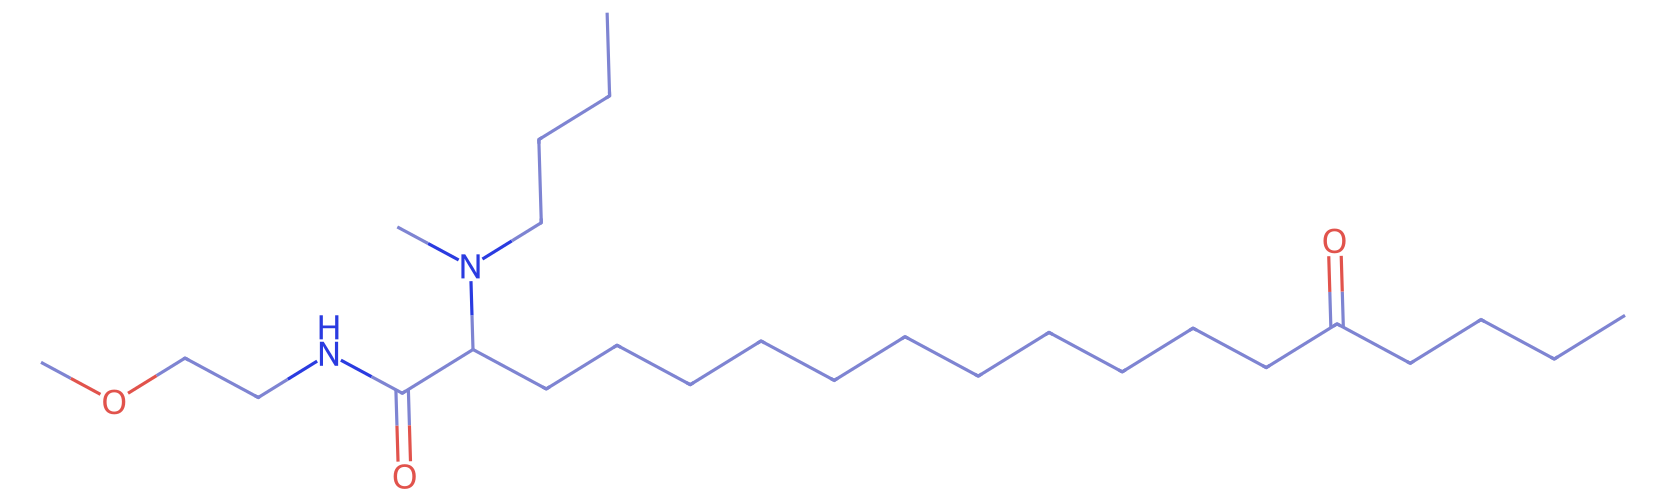
\includegraphics[width=\linewidth,height=\atlasgraphheight,keepaspectratio]{figures/forge_generated_sample_atlas_v1/forge_generated_atlas_row_01_2d.png}
\par\vspace{\atlassmilesskip}
{\atlassmilesstyle CCCCC(=O)CCCCCCCCCCCC(C(=O)N\allowbreak{}CCOC)N(C)CCCC\par}
\end{minipage}
&
\begin{minipage}[c][\atlasrowheight][c]{\atlasviewwidth}
\centering
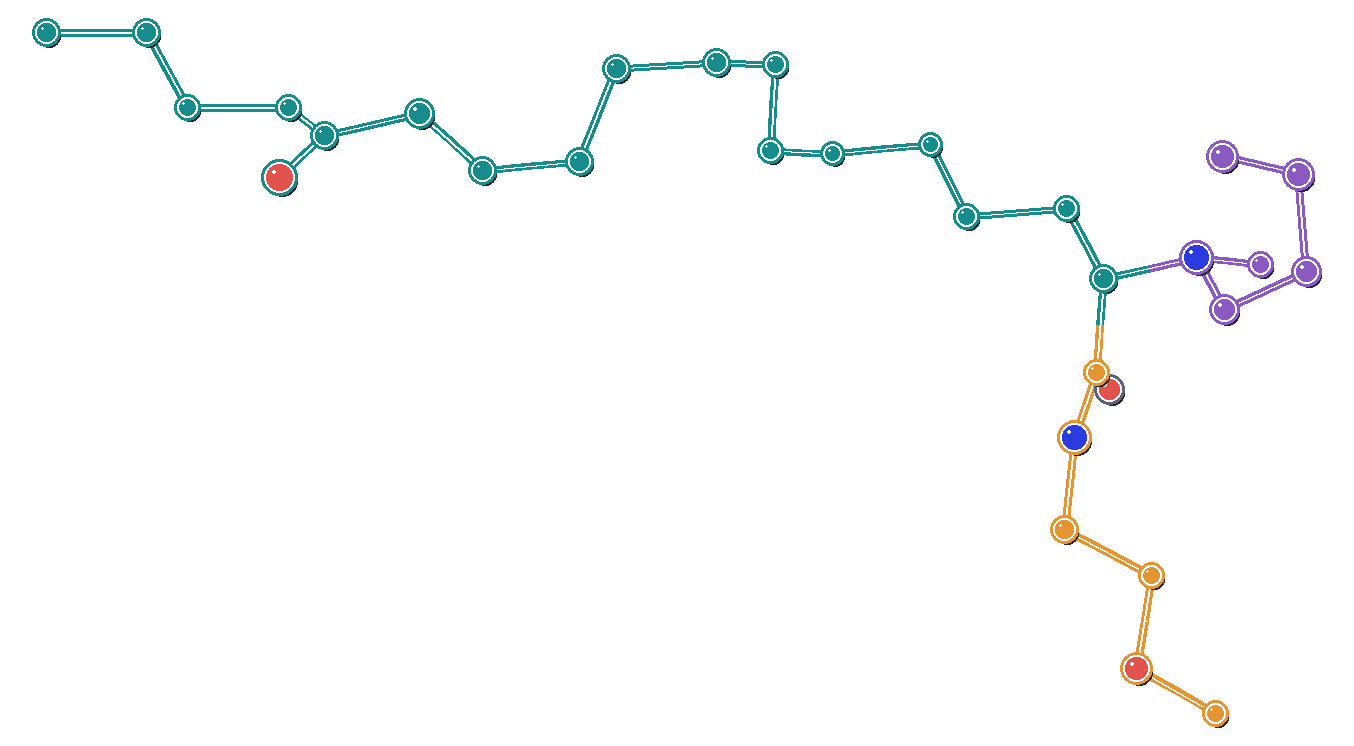
\includegraphics[width=\linewidth,height=\atlasviewheight,keepaspectratio]{figures/forge_generated_sample_atlas_v1/forge_generated_atlas_row_01_3d.png}
\end{minipage}\\
\atlasrank{2}
&
\begin{minipage}[c][\atlasrowheight][c]{\atlasgraphwidth}
\centering
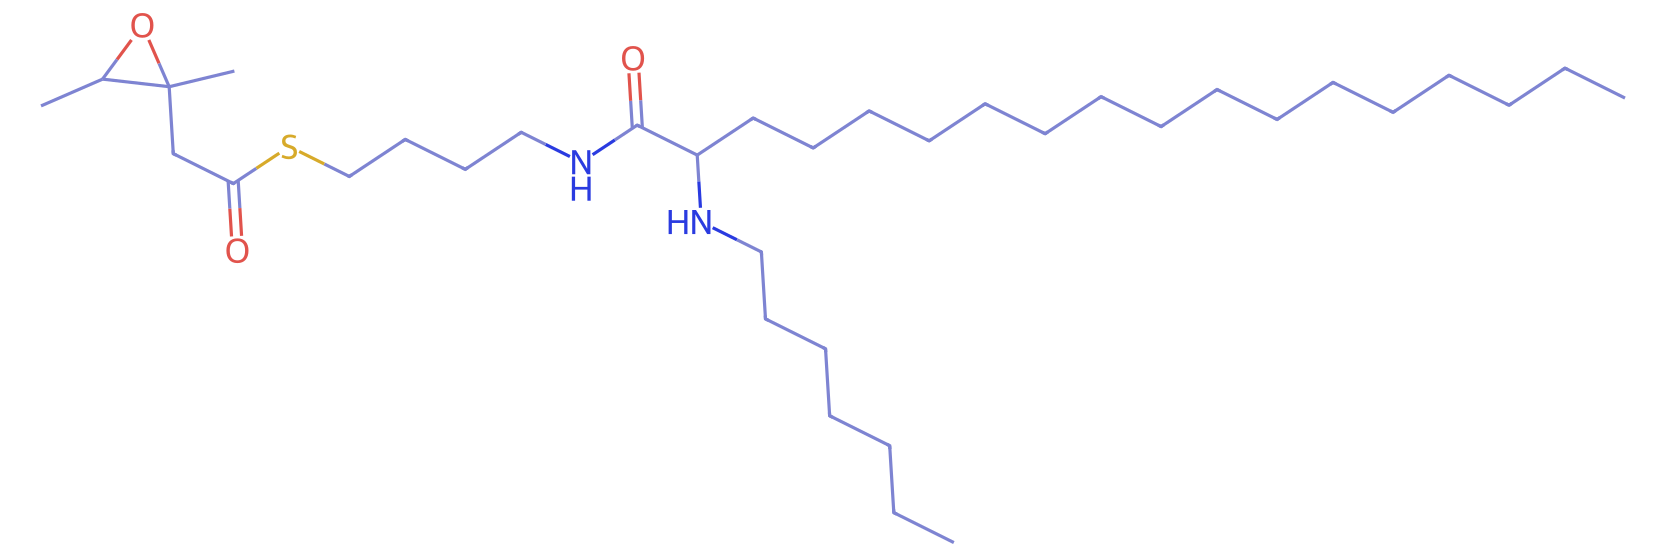
\includegraphics[width=\linewidth,height=\atlasgraphheight,keepaspectratio]{figures/forge_generated_sample_atlas_v1/forge_generated_atlas_row_02_2d.png}
\par\vspace{\atlassmilesskip}
{\atlassmilesstyle CCCCCCCCCCCCCCCCC(NCCCCCCC)C\allowbreak{}(=O)NCCCCSC(=O)CC1(C)OC1C\par}
\end{minipage}
&
\begin{minipage}[c][\atlasrowheight][c]{\atlasviewwidth}
\centering
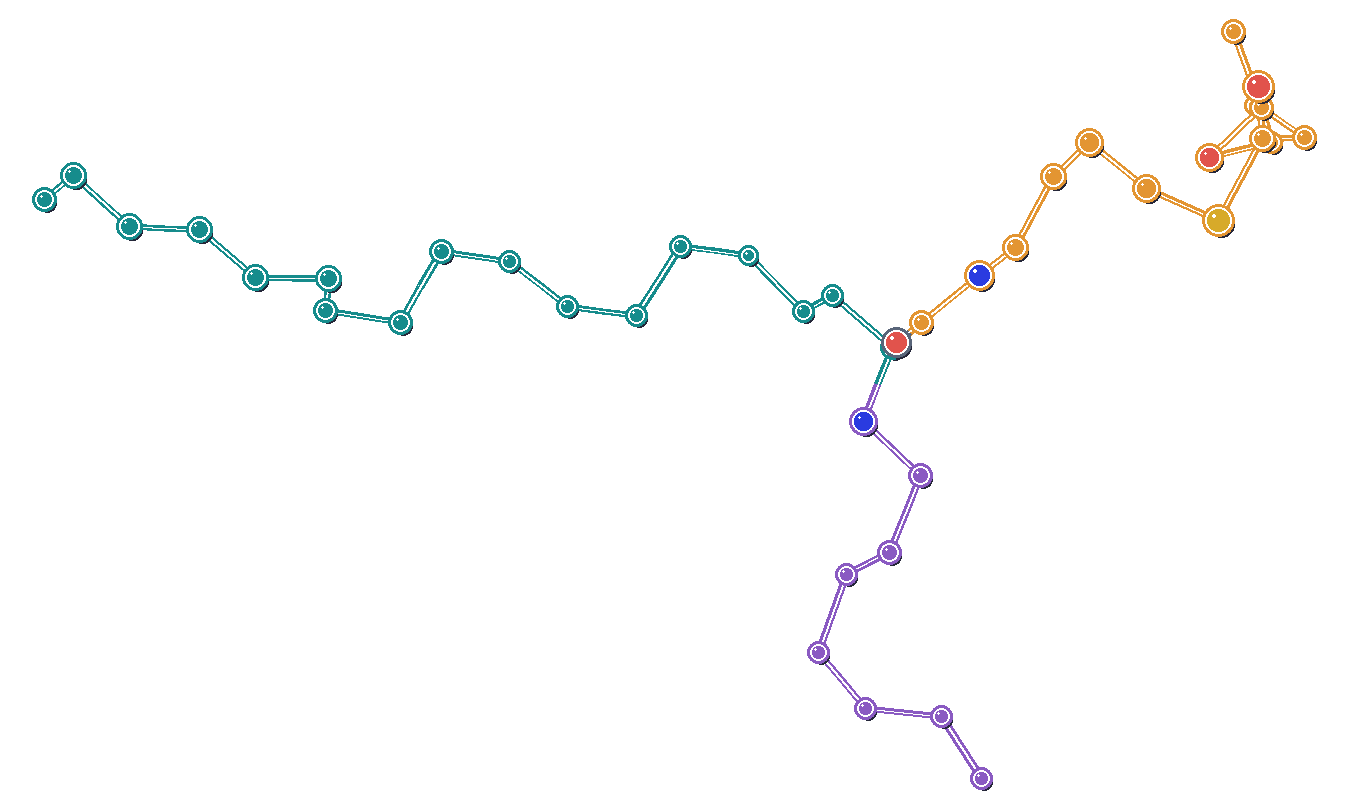
\includegraphics[width=\linewidth,height=\atlasviewheight,keepaspectratio]{figures/forge_generated_sample_atlas_v1/forge_generated_atlas_row_02_3d.png}
\end{minipage}\\
\atlasrank{3}
&
\begin{minipage}[c][\atlasrowheight][c]{\atlasgraphwidth}
\centering
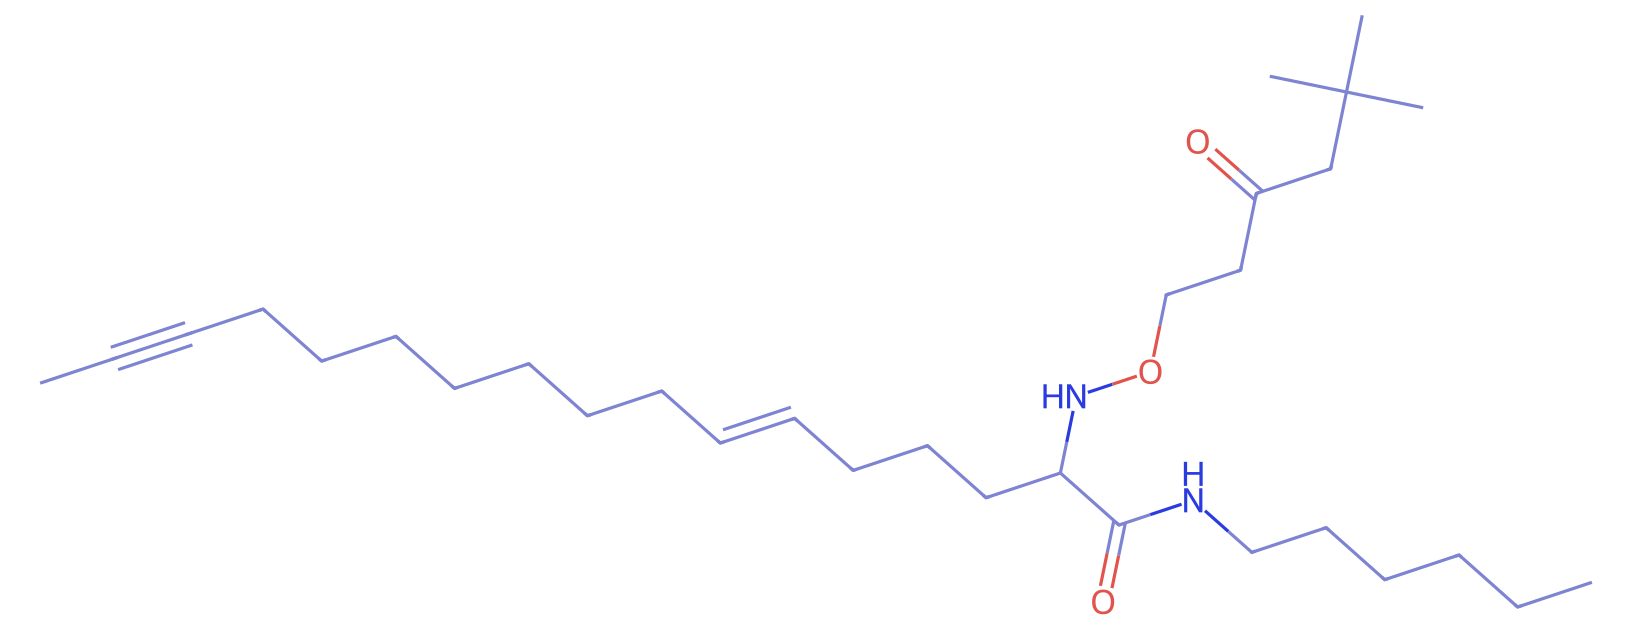
\includegraphics[width=\linewidth,height=\atlasgraphheight,keepaspectratio]{figures/forge_generated_sample_atlas_v1/forge_generated_atlas_row_03_2d.png}
\par\vspace{\atlassmilesskip}
{\atlassmilesstyle CC\#CCCCCCCCC=CCCCC(NOCCC(=O)\allowbreak{}CC(C)(C)C)C(=O)NCCCCCC\par}
\end{minipage}
&
\begin{minipage}[c][\atlasrowheight][c]{\atlasviewwidth}
\centering
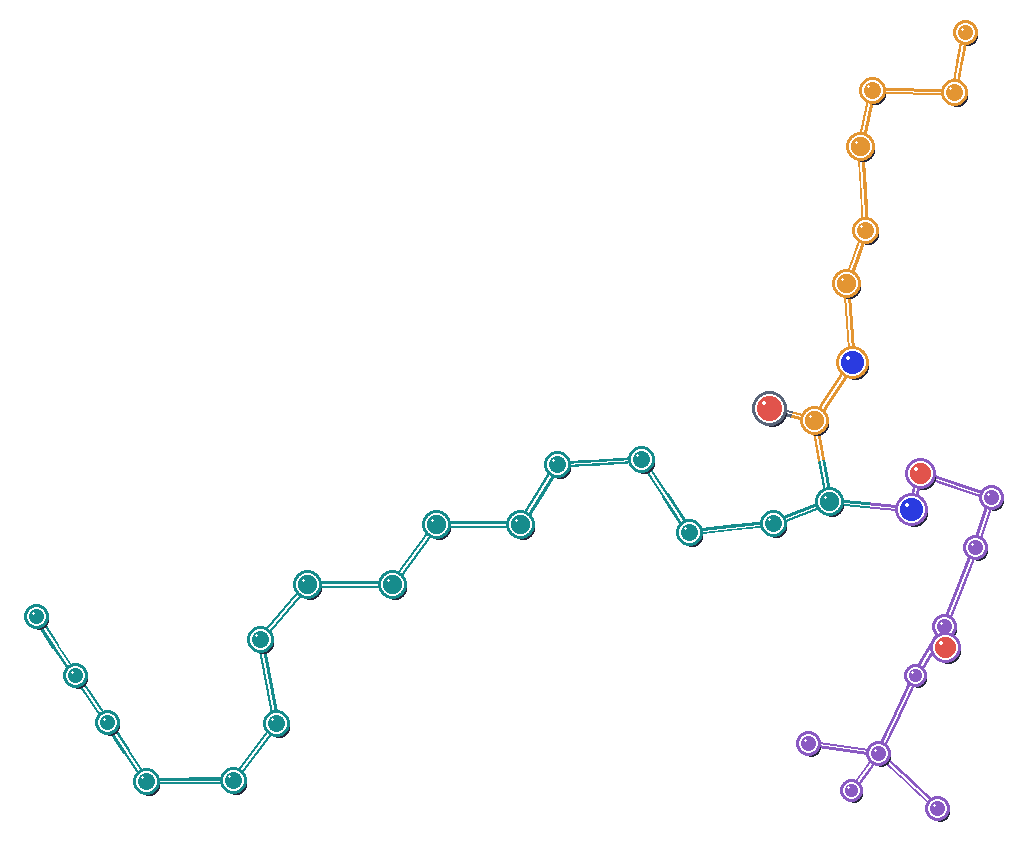
\includegraphics[width=\linewidth,height=\atlasviewheight,keepaspectratio]{figures/forge_generated_sample_atlas_v1/forge_generated_atlas_row_03_3d.png}
\end{minipage}\\
\atlasrank{4}
&
\begin{minipage}[c][\atlasrowheight][c]{\atlasgraphwidth}
\centering
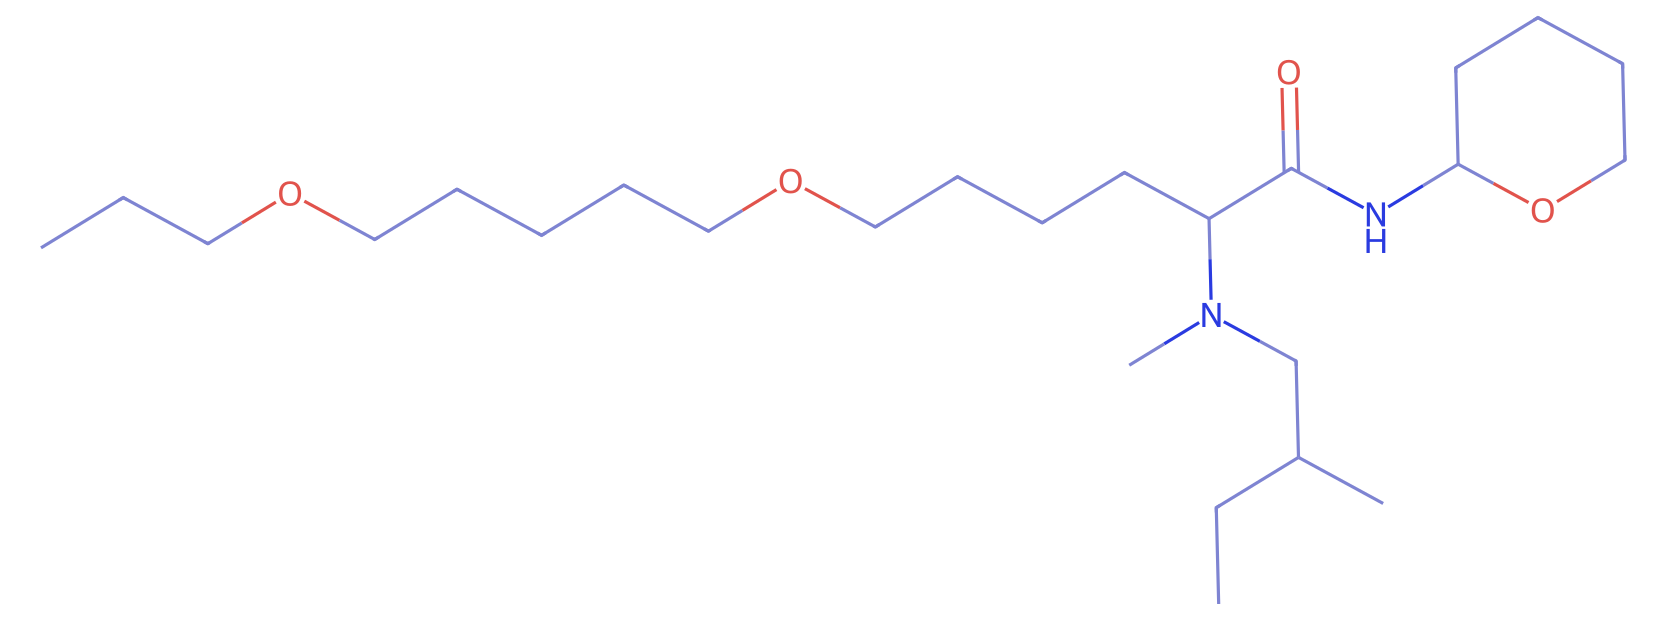
\includegraphics[width=\linewidth,height=\atlasgraphheight,keepaspectratio]{figures/forge_generated_sample_atlas_v1/forge_generated_atlas_row_04_2d.png}
\par\vspace{\atlassmilesskip}
{\atlassmilesstyle CCCOCCCCCOCCCCC(C(=O)NC1CCCC\allowbreak{}O1)N(C)CC(C)CC\par}
\end{minipage}
&
\begin{minipage}[c][\atlasrowheight][c]{\atlasviewwidth}
\centering
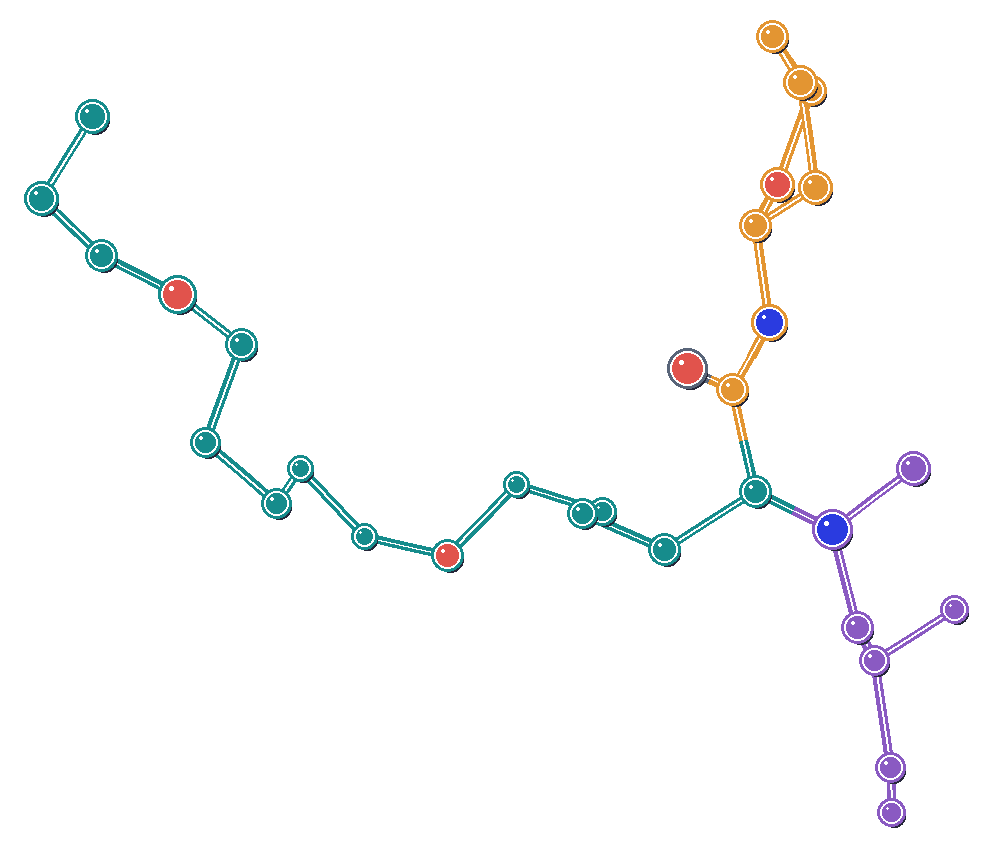
\includegraphics[width=\linewidth,height=\atlasviewheight,keepaspectratio]{figures/forge_generated_sample_atlas_v1/forge_generated_atlas_row_04_3d.png}
\end{minipage}\\
\atlasrank{5}
&
\begin{minipage}[c][\atlasrowheight][c]{\atlasgraphwidth}
\centering
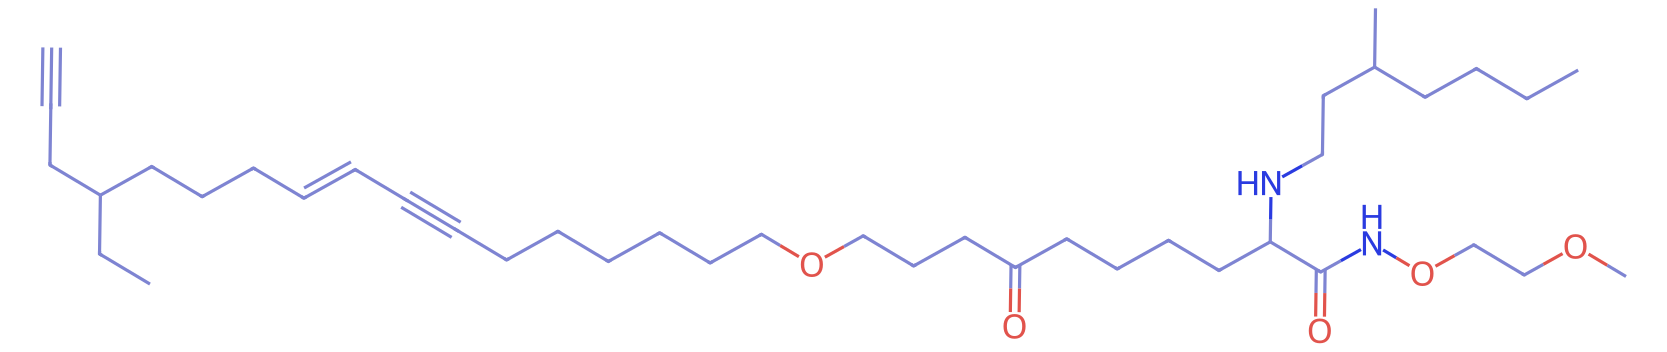
\includegraphics[width=\linewidth,height=\atlasgraphheight,keepaspectratio]{figures/forge_generated_sample_atlas_v1/forge_generated_atlas_row_05_2d.png}
\par\vspace{\atlassmilesskip}
{\atlassmilesstyle C\#CCC(CC)CCCC=CC\#CCCCCCCOCCC\allowbreak{}C(=O)CCCCC(NCCC(C)CCCC)C(=O)\allowbreak{}NOCCOC\par}
\end{minipage}
&
\begin{minipage}[c][\atlasrowheight][c]{\atlasviewwidth}
\centering
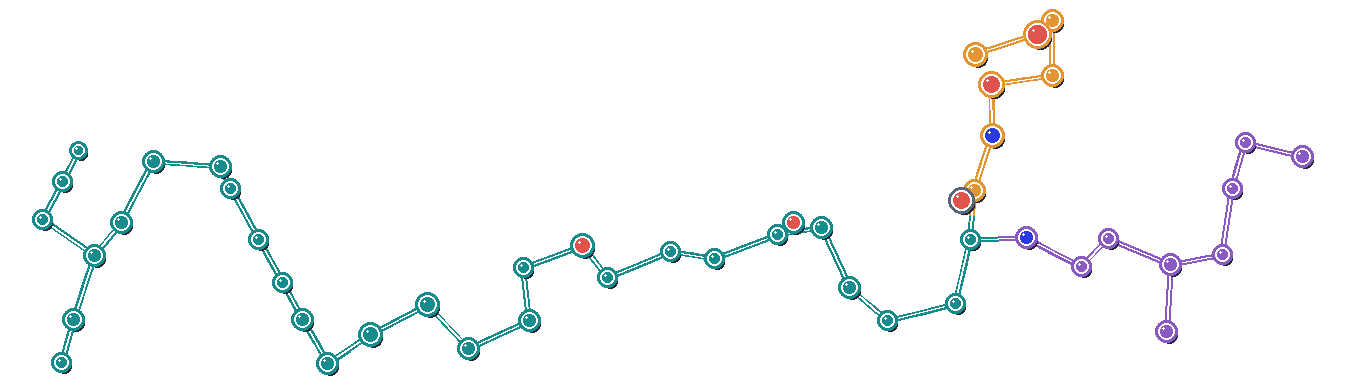
\includegraphics[width=\linewidth,height=\atlasviewheight,keepaspectratio]{figures/forge_generated_sample_atlas_v1/forge_generated_atlas_row_05_3d.png}
\end{minipage}\\
\atlasrank{6}
&
\begin{minipage}[c][\atlasrowheight][c]{\atlasgraphwidth}
\centering
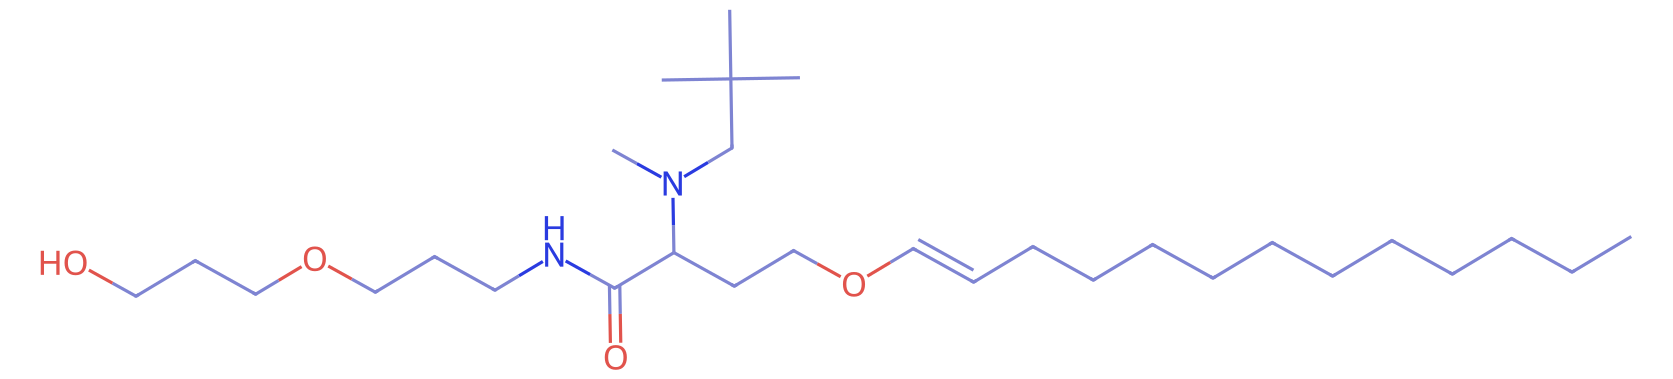
\includegraphics[width=\linewidth,height=\atlasgraphheight,keepaspectratio]{figures/forge_generated_sample_atlas_v1/forge_generated_atlas_row_06_2d.png}
\par\vspace{\atlassmilesskip}
{\atlassmilesstyle CCCCCCCCCCCC=COCCC(C(=O)NCCC\allowbreak{}OCCCO)N(C)CC(C)(C)C\par}
\end{minipage}
&
\begin{minipage}[c][\atlasrowheight][c]{\atlasviewwidth}
\centering
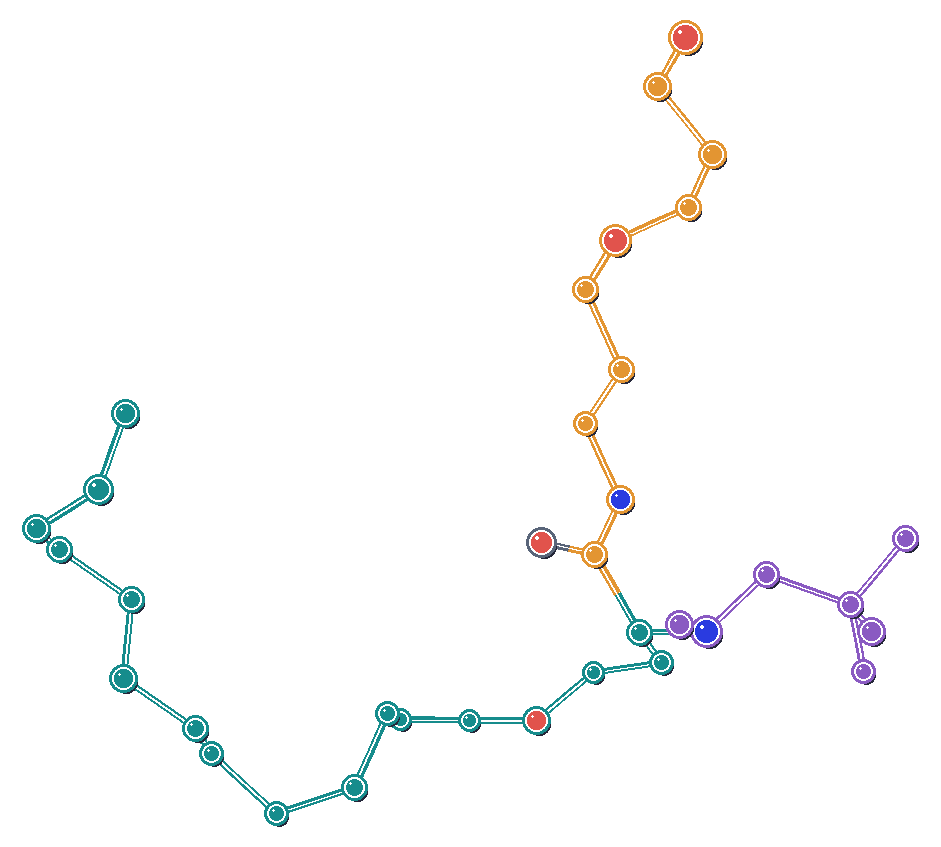
\includegraphics[width=\linewidth,height=\atlasviewheight,keepaspectratio]{figures/forge_generated_sample_atlas_v1/forge_generated_atlas_row_06_3d.png}
\end{minipage}\\
\atlasrank{7}
&
\begin{minipage}[c][\atlasrowheight][c]{\atlasgraphwidth}
\centering
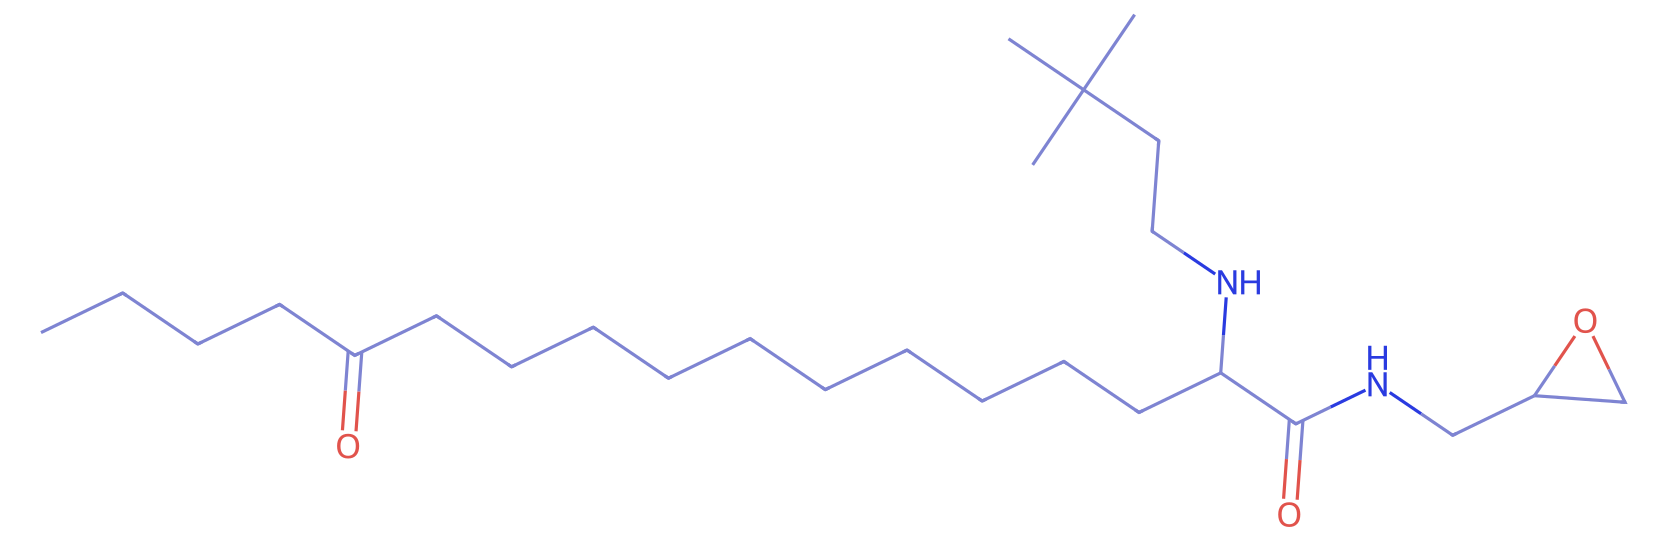
\includegraphics[width=\linewidth,height=\atlasgraphheight,keepaspectratio]{figures/forge_generated_sample_atlas_v1/forge_generated_atlas_row_07_2d.png}
\par\vspace{\atlassmilesskip}
{\atlassmilesstyle CCCCC(=O)CCCCCCCCCCC(NCCC(C)\allowbreak{}(C)C)C(=O)NCC1CO1\par}
\end{minipage}
&
\begin{minipage}[c][\atlasrowheight][c]{\atlasviewwidth}
\centering
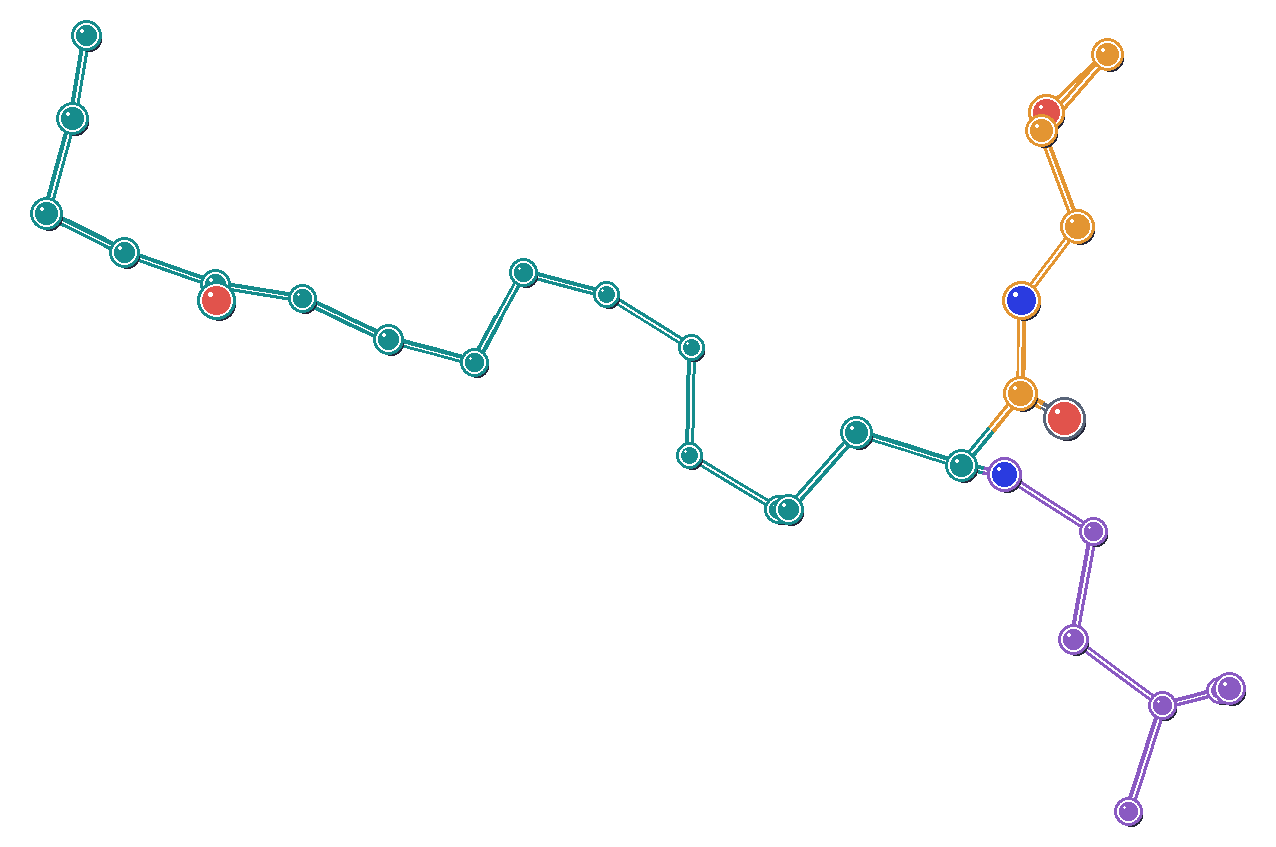
\includegraphics[width=\linewidth,height=\atlasviewheight,keepaspectratio]{figures/forge_generated_sample_atlas_v1/forge_generated_atlas_row_07_3d.png}
\end{minipage}\\
\atlasrank{8}
&
\begin{minipage}[c][\atlasrowheight][c]{\atlasgraphwidth}
\centering
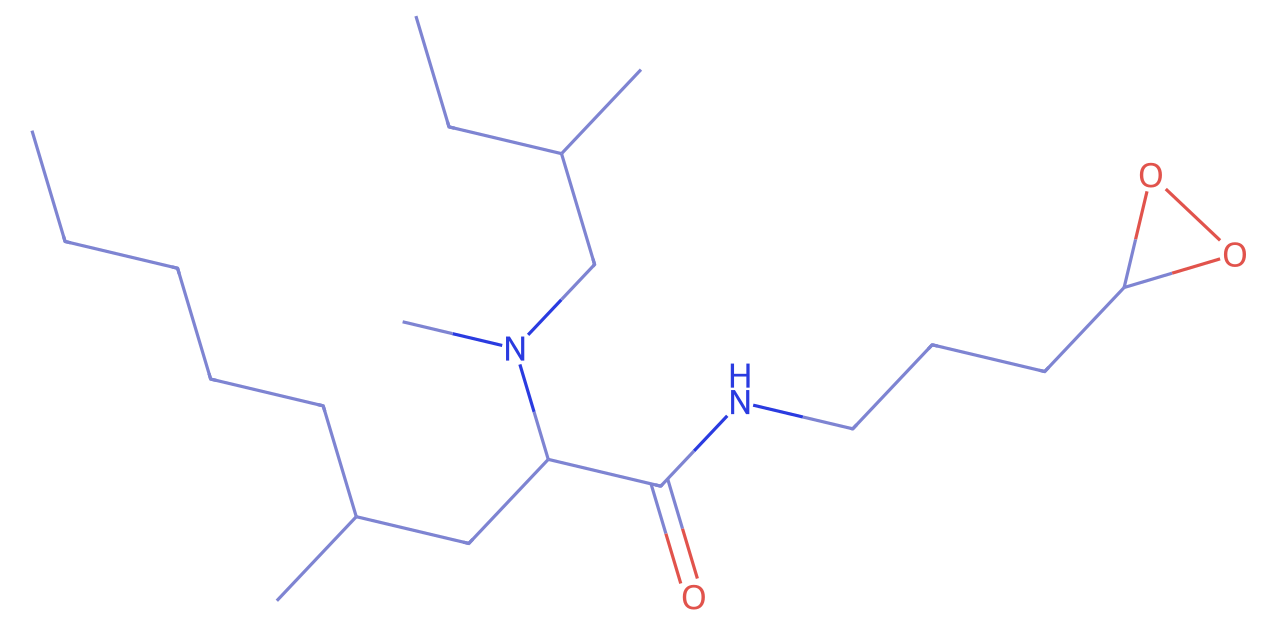
\includegraphics[width=\linewidth,height=\atlasgraphheight,keepaspectratio]{figures/forge_generated_sample_atlas_v1/forge_generated_atlas_row_08_2d.png}
\par\vspace{\atlassmilesskip}
{\atlassmilesstyle CCCCCC(C)CC(C(=O)NCCCC1OO1)N\allowbreak{}(C)CC(C)CC\par}
\end{minipage}
&
\begin{minipage}[c][\atlasrowheight][c]{\atlasviewwidth}
\centering
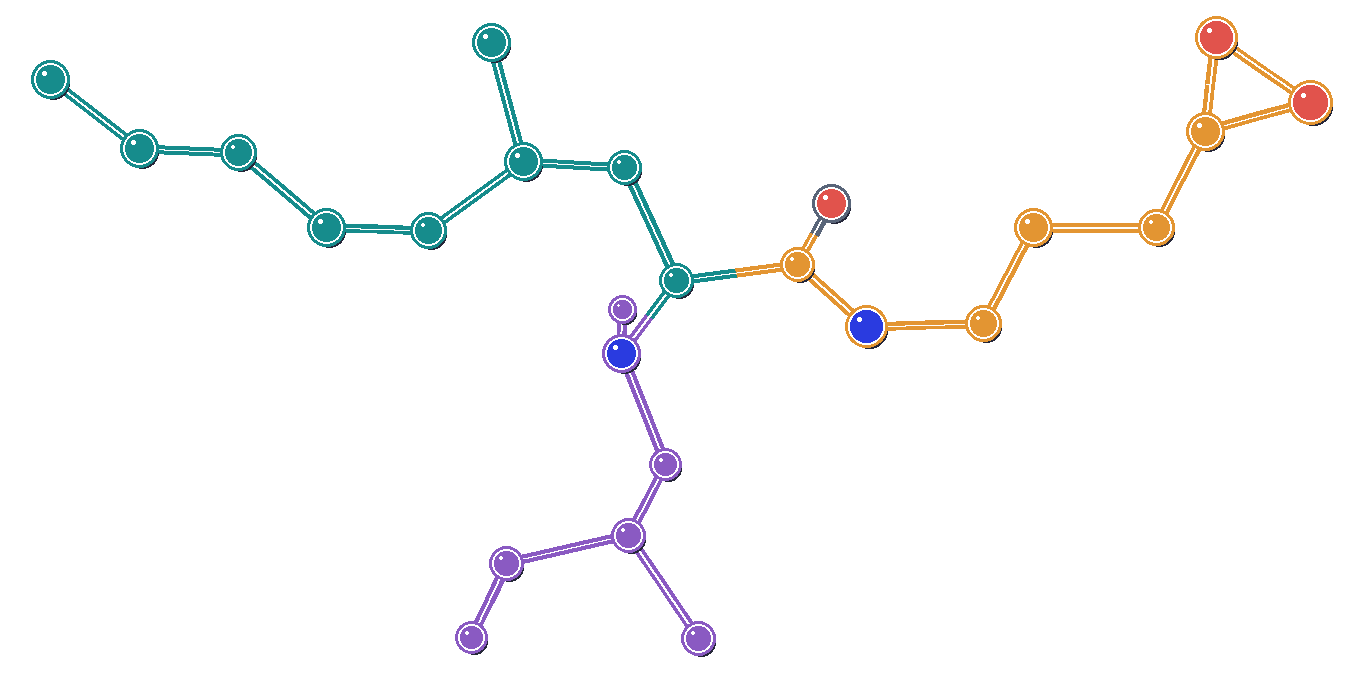
\includegraphics[width=\linewidth,height=\atlasviewheight,keepaspectratio]{figures/forge_generated_sample_atlas_v1/forge_generated_atlas_row_08_3d.png}
\end{minipage}\\
\atlasrank{9}
&
\begin{minipage}[c][\atlasrowheight][c]{\atlasgraphwidth}
\centering
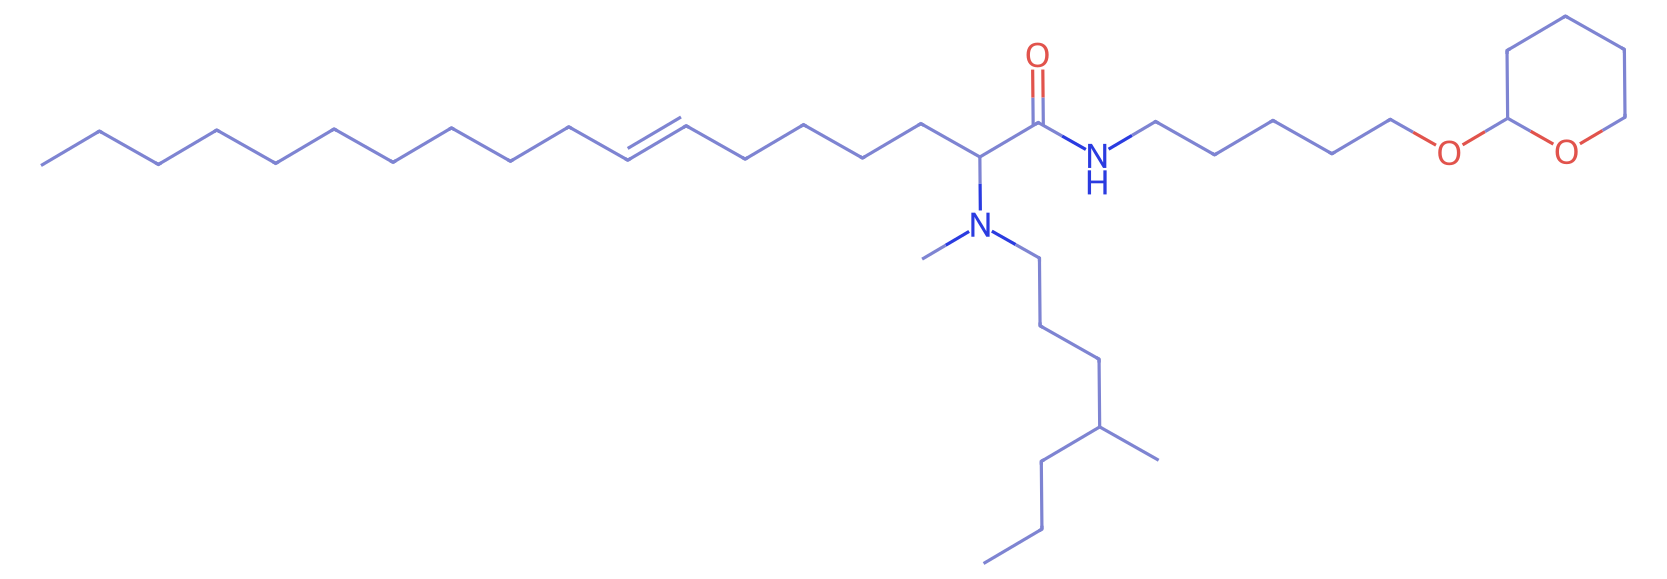
\includegraphics[width=\linewidth,height=\atlasgraphheight,keepaspectratio]{figures/forge_generated_sample_atlas_v1/forge_generated_atlas_row_09_2d.png}
\par\vspace{\atlassmilesskip}
{\atlassmilesstyle CCCCCCCCCCC=CCCCCC(C(=O)NCCC\allowbreak{}CCOC1CCCCO1)N(C)CCCC(C)CCC\par}
\end{minipage}
&
\begin{minipage}[c][\atlasrowheight][c]{\atlasviewwidth}
\centering
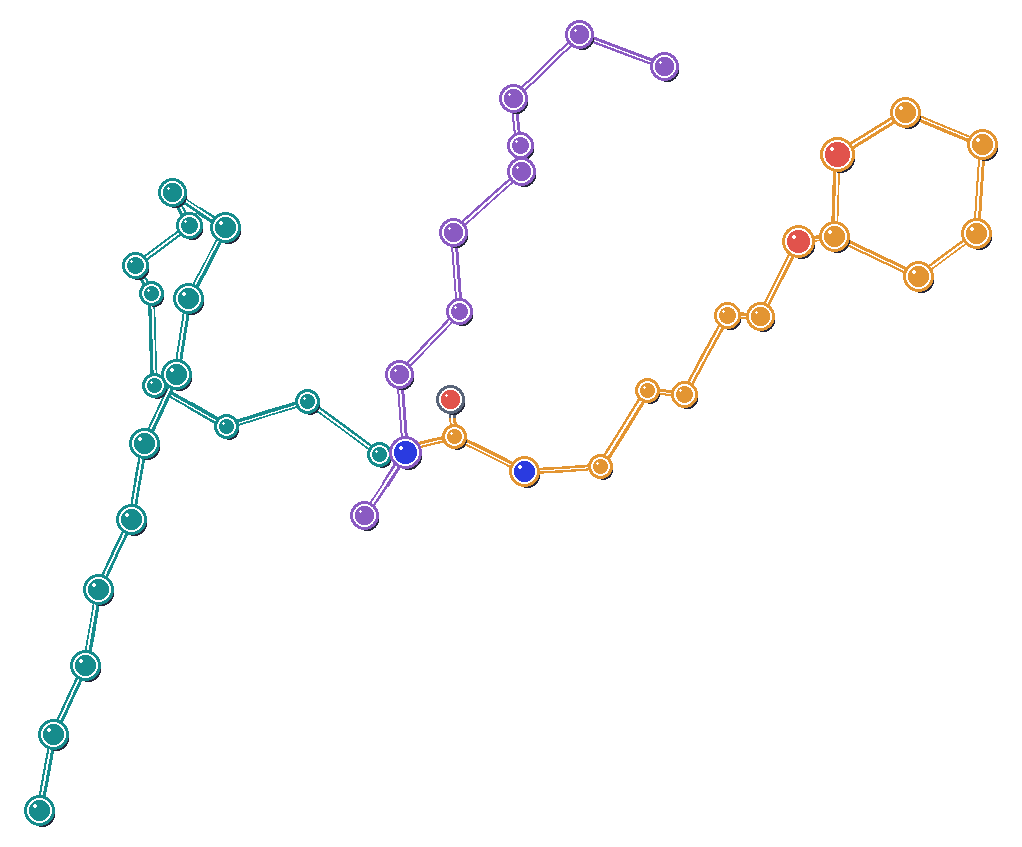
\includegraphics[width=\linewidth,height=\atlasviewheight,keepaspectratio]{figures/forge_generated_sample_atlas_v1/forge_generated_atlas_row_09_3d.png}
\end{minipage}\\
\atlasrank{10}
&
\begin{minipage}[c][\atlasrowheight][c]{\atlasgraphwidth}
\centering
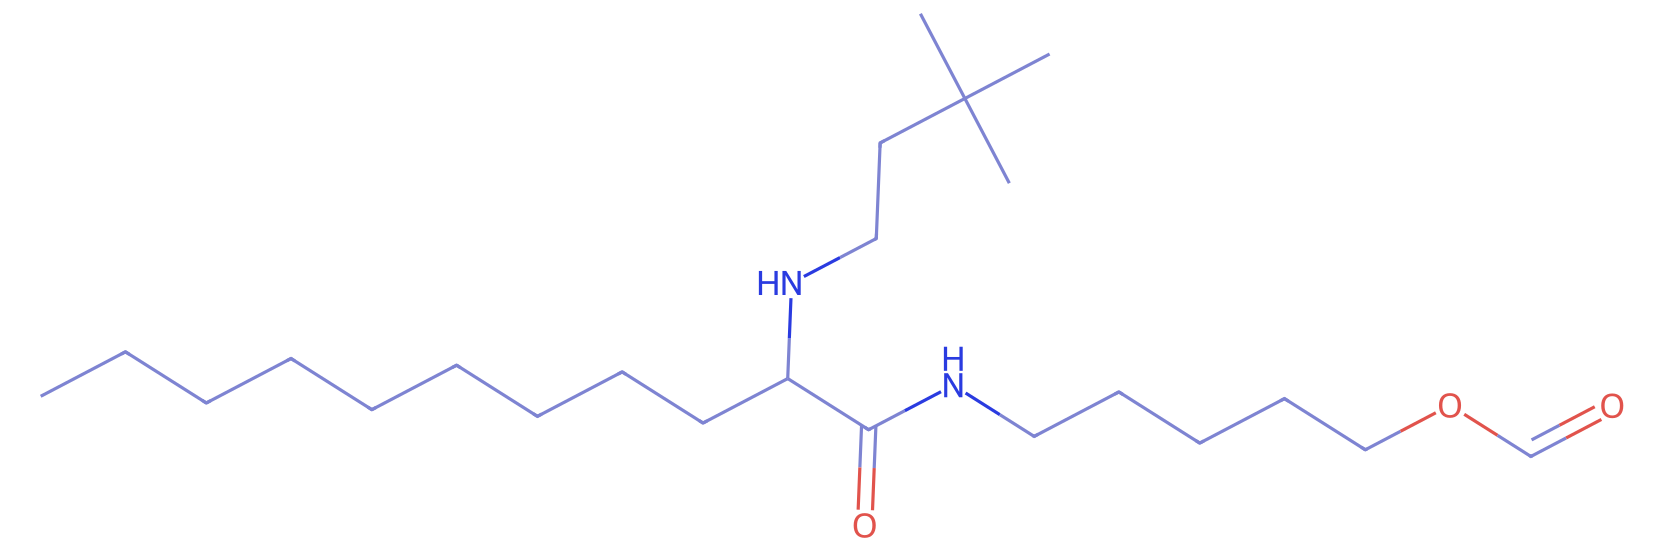
\includegraphics[width=\linewidth,height=\atlasgraphheight,keepaspectratio]{figures/forge_generated_sample_atlas_v1/forge_generated_atlas_row_10_2d.png}
\par\vspace{\atlassmilesskip}
{\atlassmilesstyle CCCCCCCCCC(NCCC(C)(C)C)C(=O)\allowbreak{}NCCCCCOC=O\par}
\end{minipage}
&
\begin{minipage}[c][\atlasrowheight][c]{\atlasviewwidth}
\centering
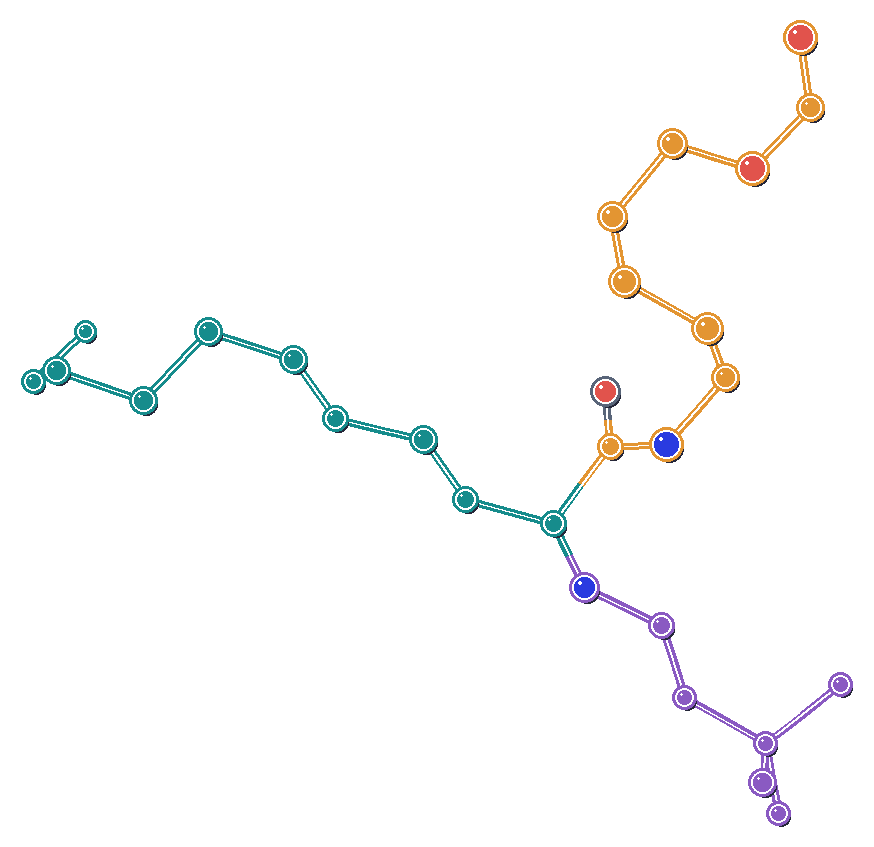
\includegraphics[width=\linewidth,height=\atlasviewheight,keepaspectratio]{figures/forge_generated_sample_atlas_v1/forge_generated_atlas_row_10_3d.png}
\end{minipage}\\
\atlasrank{11}
&
\begin{minipage}[c][\atlasrowheight][c]{\atlasgraphwidth}
\centering
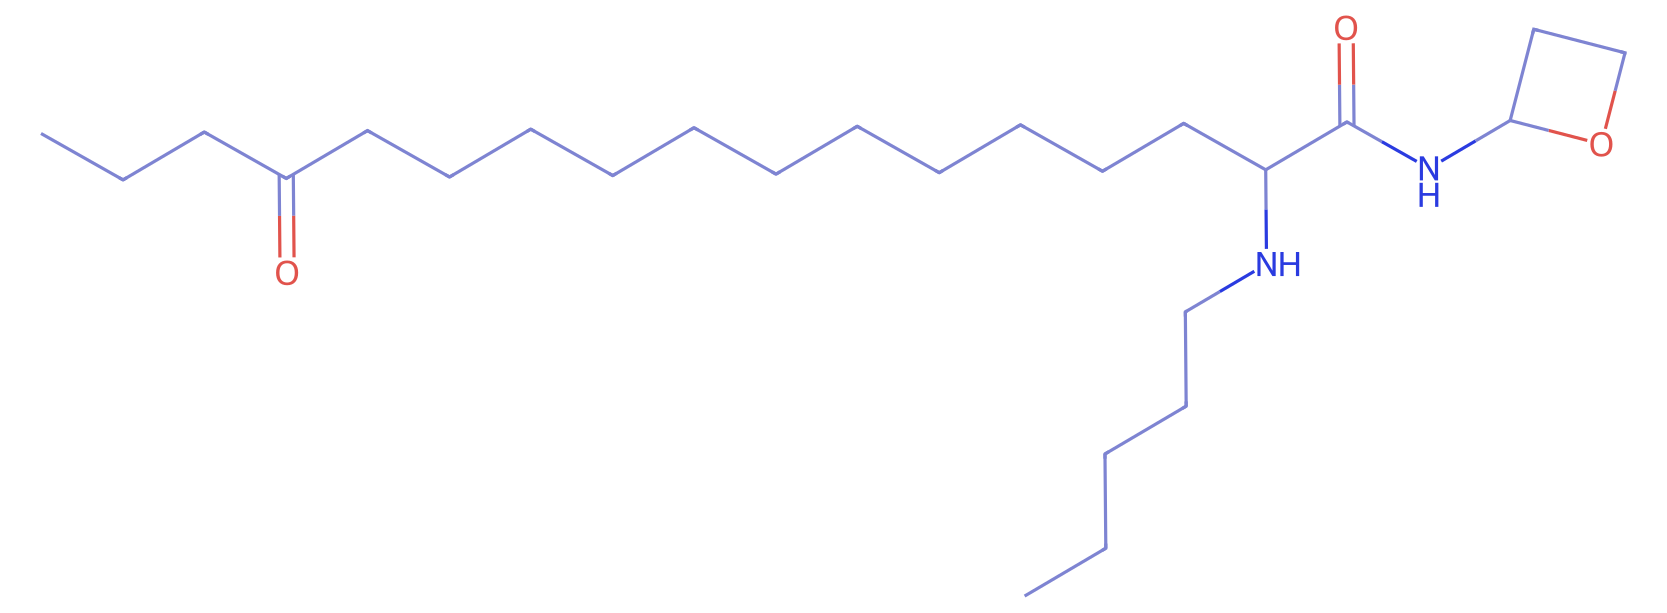
\includegraphics[width=\linewidth,height=\atlasgraphheight,keepaspectratio]{figures/forge_generated_sample_atlas_v1/forge_generated_atlas_row_11_2d.png}
\par\vspace{\atlassmilesskip}
{\atlassmilesstyle CCCCCNC(CCCCCCCCCCCC(=O)CCC)\allowbreak{}C(=O)NC1CCO1\par}
\end{minipage}
&
\begin{minipage}[c][\atlasrowheight][c]{\atlasviewwidth}
\centering
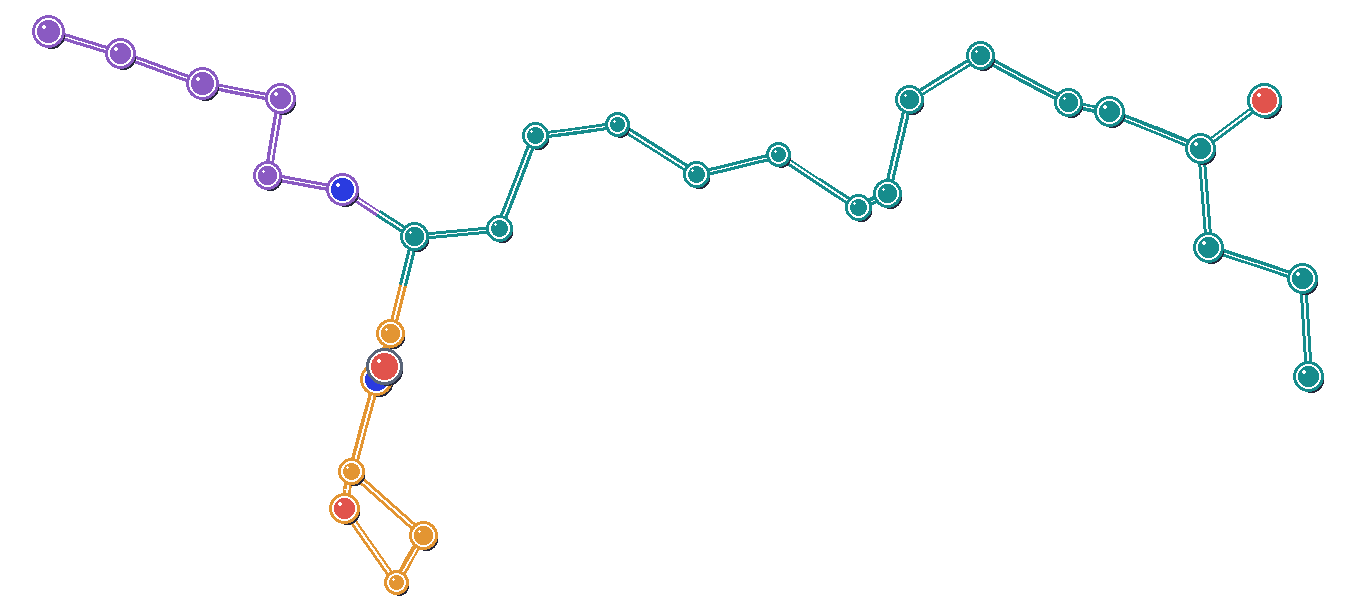
\includegraphics[width=\linewidth,height=\atlasviewheight,keepaspectratio]{figures/forge_generated_sample_atlas_v1/forge_generated_atlas_row_11_3d.png}
\end{minipage}\\
\atlasrank{12}
&
\begin{minipage}[c][\atlasrowheight][c]{\atlasgraphwidth}
\centering
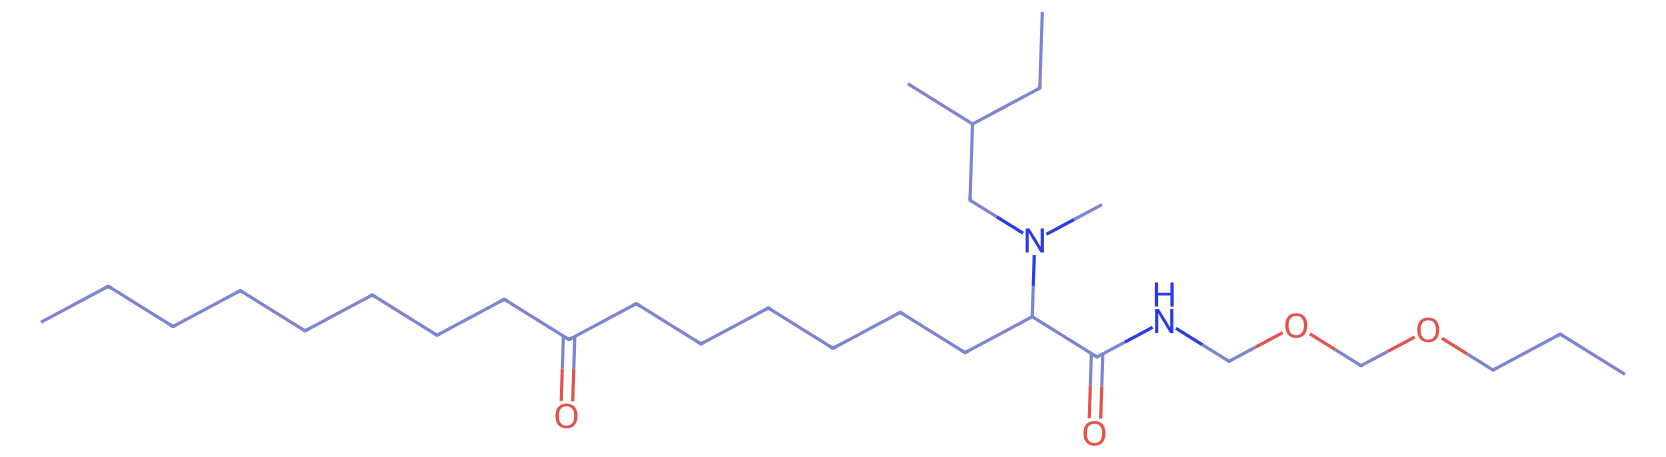
\includegraphics[width=\linewidth,height=\atlasgraphheight,keepaspectratio]{figures/forge_generated_sample_atlas_v1/forge_generated_atlas_row_12_2d.png}
\par\vspace{\atlassmilesskip}
{\atlassmilesstyle CCCCCCCCC(=O)CCCCCCC(C(=O)NC\allowbreak{}OCOCCC)N(C)CC(C)CC\par}
\end{minipage}
&
\begin{minipage}[c][\atlasrowheight][c]{\atlasviewwidth}
\centering
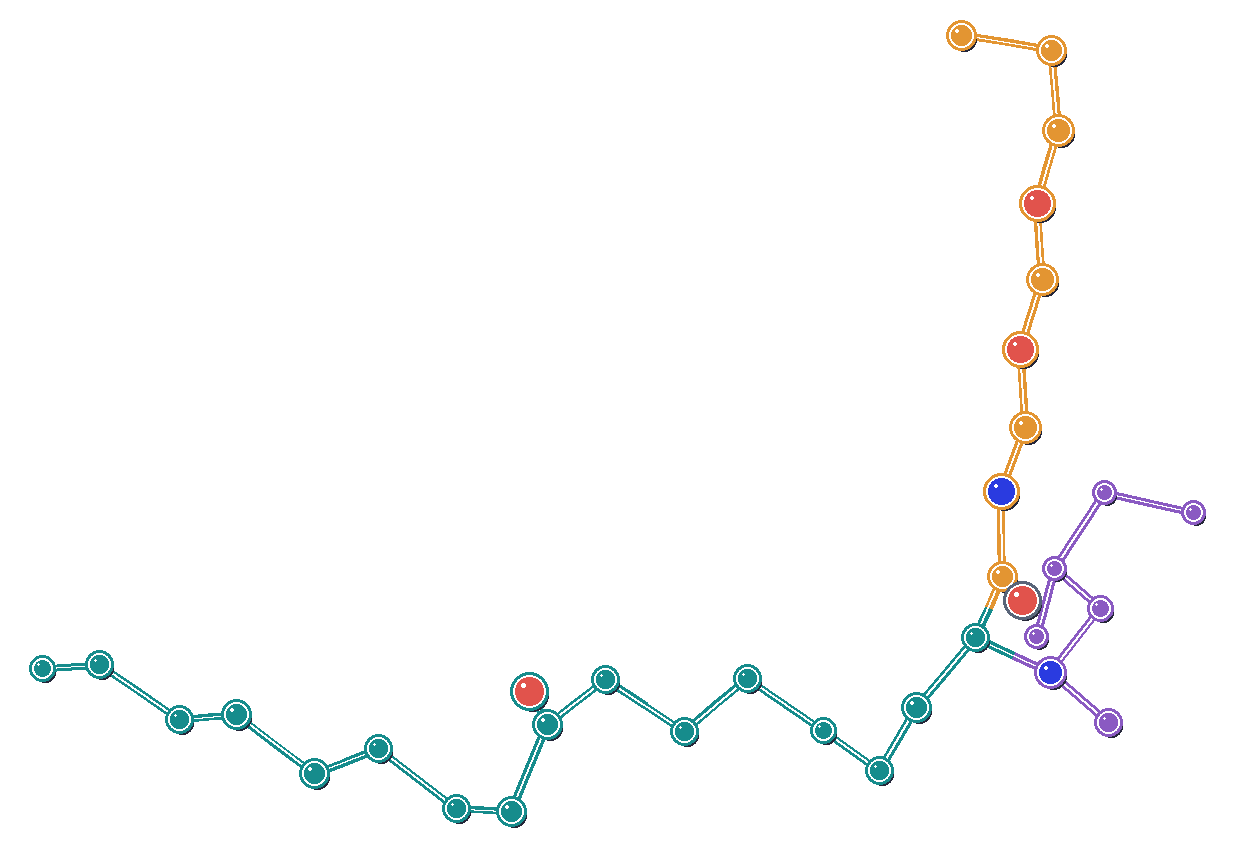
\includegraphics[width=\linewidth,height=\atlasviewheight,keepaspectratio]{figures/forge_generated_sample_atlas_v1/forge_generated_atlas_row_12_3d.png}
\end{minipage}\\
%
\end{longtable}
\endgroup


\end{document}
